\documentclass[mscthesis]{usiinfthesis}
\usepackage{lipsum}
\usepackage{listings}
\usepackage{pdfpages}
\usepackage{subcaption}
\usepackage{graphicx}

\usepackage{hyperref}
\usepackage{changepage}
\usepackage[utf8]{inputenc}

\lstdefinelanguage{algebra}
{morekeywords={import,sort,constructors,observers,transformers,axioms,if,
else,end},
sensitive=false,
morecomment=[l]{//s},
}



\title{Evaluating Secure Personal Memory Sharing with co-located people} %compulsory
%\specialization{Management and Informatics}%optional 
\author{Jacob Jeyaraj} %compulsory
\begin{committee}
\advisor{Prof.}{Marc}{Langheinrich} %compulsory
\coadvisor{}{Agon}{Bexheti}{} %optional
\end{committee}
\Day{01} %compulsory
\Month{February} %compulsoryx
\Year{2018} %compulsory, put only the year
\place{Lugano} %compulsory

\dedication{To my family} %optional
\openepigraph{Be the change you want to see in the world.}{Mahatma Gandhi} %optional

%\makeindex %optional, also comment out \theindex at the end

\begin{document}

\maketitle %generates the titlepage, this is FIXED

\frontmatter %generates the frontmatter, this is FIXED

\begin{abstract}
Throughout history, people have recorded parts of their daily activities in journals and diaries to preserve their experiences. Modern technology allows us to capture more aspects of our mundane activities in a digital format, a process known as "lifelogging". There are many findings suggesting that lifelogging can help to augment or improve human memory. A recently finished project, "RECALL" aimed at harnessing such lifelogs and develop new technologies for augmenting human memory. "MemShare" is one such technology that does not only capture one's own memories (as images) of an event (using body-worn cameras), but it also seamlessly and securely shares them with all users that are experiencing the same moment together.

Since the MemShare system acquires vast quantities of lifelog data from the user and from co-located peers, this requires a user interface to efficiently present and visualize the lifelog contents from the MemShare system. Therefore, as part of this thesis a prototype website was designed with a novel web user interface to manage and present the lifelog contents in a visually less complex way. The design of the prototype website was evaluated by users and verified users could could efficiently navigate and display the lifelog contents. The evaluation showed that users overall liked the presentation of information in the prototype website but they identified some usability problems and they gave suggestions to help further improve the design of the website in the future. 

Users can operate the MemShare architecture using a tangible user interface, called MemStone. This device acts like a controller which allows users to control some aspects of data capture and sharing. Another part of this thesis is to evaluate MemStone's usability and user experience. This evaluation is done to understand the use, usability requirements and to collect feedback and suggestions to further refine the device and the whole system. From the evaluation, the strengths and weaknesses of the MemStone device were identified and several ideas to improve the device and the system were also identified. The findings from this thesis can be used to refine the overall system, giving ideas and suggestions to design a better MemStone device and as well as designing proper web user interface to view the lifelog contents.

\end{abstract}

\begin{acknowledgements}
I would like to take this opportunity to thank all the people who had supported and helped me to complete my thesis. I especially thank Prof.Marc Langheinrich for giving me the opportunity to do my research. I am very grateful to Agon Bexheti for guiding me through every step for my thesis and giving me valuable advice on how to do my research experiments. I would like to thank my family and my girlfriend for encouraging me and giving me the support. Finally, I would like to thank my friends and family who helped me to complete my research study by spending their time on taking part in the study and giving their valuable feedback. 
\end{acknowledgements}

\tableofcontents 
\listoffigures %optional
\listoftables %optional

\mainmatter

\chapter{Introduction}

Nowadays people feel more urged to digitally record everything that is happening in their lives and save in a digital form. This phenomenon is known as lifelogging where all kinds of personal data such as location, emotional states, physical performance etc., are captured or recorded automatically using lifelogging devices (wearable cameras, fitness devices, non-wearable devices and so on). Some of these wearable devices can be seen in the market, especially predominant in health and fitness industry like the Samsung Gear fit \footnote{\url{https://www.samsung.com/us/explore/gear-fit2-pro/}} and FitBit \footnote{\url{https://www.fitbit.com/eu/home}}. There are many applications of 
such devices, also known as "quantified-self". For example, some of these devices track physical activity of a user to show information on how much time they have spent exercising or how many steps they have climbed on a day. Using this data, users can self-reflect and improve his performance in the future. Lifelogging is not only restricted to GPS and psychological personal data, but it also focuses on capturing images or recording videos.

\begin{figure}[!ht]
  \centering
  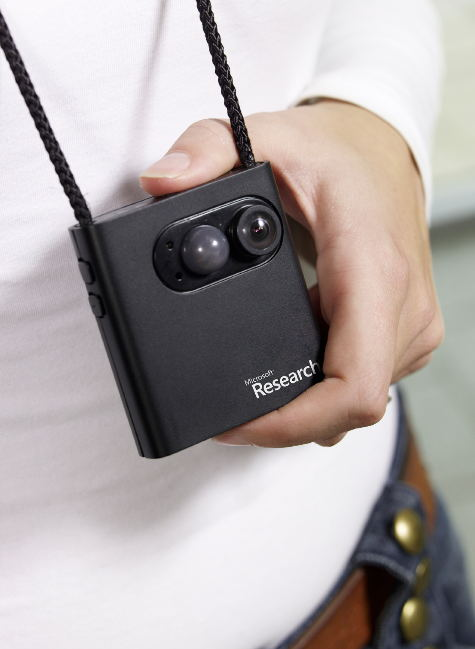
\includegraphics[width=0.3\textwidth]{sensecam}
  \caption{SenseCam; Source: \url{https://www.microsoft.com/en-us/research/project/sensecam/}.}
  \label{fig0}
\end{figure}

One of the earliest lifelogging device to automatically capture images is SenseCam (fig.\ref{fig0}). It was developed in 2004 and it automatically captures images from a first-person perspective. By default, SenseCam captures images for every 40 seconds of a person's day to day life to create a visual lifelog consisting of between 3500 to 4500 images. These captured images provides a rich contextual information of one's life and this information can be used to trigger memories of past experiences \citep{gurrin_lifelogging:_2014}. There were many studies conducted using SenseCam which proved that lifelogging technologies can aid for those with chronic memory related diseases such as Amnesia and Alzheimer's  \citep{berry_use_2007} \citep{doi:10.1080/09658211.2014.886703}. Moreover, yet another study done by \citeauthor{sellen_life-logging_2007}, also proves that the images automatically captured by SenseCam served as a cue to link past memories on healthy individuals. 

The recently finished FET project RECALL \footnote{\url{http://recall-fet.eu}} harnesses these findings and the lifelogging concept to develop new memory augmentation technologies which would benefit the society. The RECALL project aimed to re-think and re-define the notion of human memory augmentation. In their recent work, \citeauthor{davies_security_2015} presented the concept of a pervasive memory augmentation system that can be used to augment human memory. They define such system as a three steps process, in the first step user's daily experiences are captured in a digital format, then it is carefully processed in order to generate 'memory cues' and finally the memory cues are presented back to users in a ambient fashion displays. The memory cue is nothing but a snippet of information (e.g., a photograph or a sound) that when reviewed has the ability to bring back memories associated to it. When it comes to memory cues, \citeauthor{dingler_multimedia_2016} have identified that images provide the most effective memory cues for recalling past memories.

Based on these works, \citeauthor{bexheti_secure_2016} have built a memory augmentation system called MemShare that not only captures experiences through user's personal wearable cameras, but it also seamlessly and securely shares such personal memories with other users that are experiencing the same event together. The system was built based on the idea from \citeauthor{clinch_lifelogging_2014} and \citeauthor{byrne_life_2011}, where they suggest that first-person view images captured from the wearable cameras of others can offer a richer view than what one's own camera does and third-person view images captured from infrastructure camera's provides even a better view of an event. Therefore, the MemShare system allows secure and automatically sharing of one's lifelog data(images) with co-located peers and captures images from fixed camera near the user. An overview of MemShare is provided in the next section \ref{sec:bac}.
 
\section{The MemShare system}
\label{sec:bac}
The MemShare system was built by \citet{bexheti_secure_2016} as part of the RECALL project. The purpose of the system was to both capture and share memories during an event (e.g., a meeting) and help the user's to recall what happened in the event when they review the captured information after. For capturing these images the system uses a lifelogging wearable camera called "Narrative Clip 2" as shown in figure \ref{fig1}. Compared with the SenseCam the Narrative Clip 2 is a small and light wearable camera which captures high quality images. This wearable camera also features a longer battery life compared to SenseCam and it can be pinned up in shirt so that it takes first person perspective images. The system works by allowing the captured images from the Narrative Clip 2 to be shared among co-located meeting attendants and vice versa. If there is any infrastructure camera available nearby the user, the system will also acquires the captured images from the infrastructure camera. This provides the user a better perspective of an event. Later the user can view all the images captured from the user's perspective, meeting attendant's perspective and infrastructure camera in a website user interface.


\begin{figure}[!ht]
  \centering
  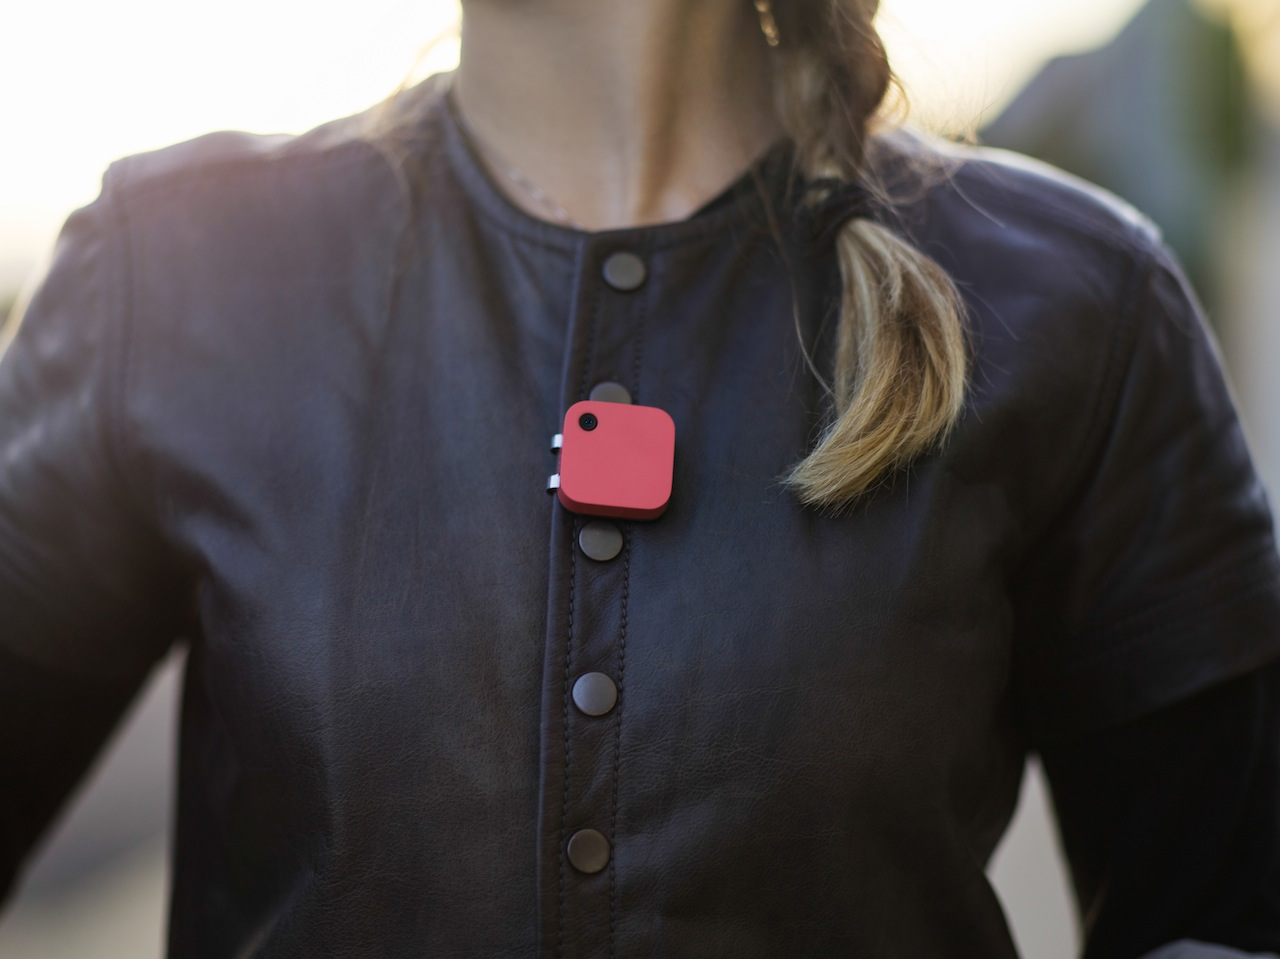
\includegraphics[width=0.5\textwidth]{Clip}
  \caption{Narrative Clip 2; Source: \url{http://www.getnarrative.com}.}
  \label{fig1}
\end{figure}

The initial prototype of the MemShare system was first implemented in an android application and this application worked on pair with Narrative Clip 2 which captures the user activities and stores it in a memory repository. In a two-user meeting scenario as shown in figure \ref{fig2}, the application works by broadcasting its willingness to share images and acquires images from others. When the application detects a nearby peer who is also willing to share and capture, it automatically initiates the exchanges of captured data location (URL of memory repository) securely with each other. The captured data (images) location from the infrastructure camera is also shared with both the peers. If the peer leaves the meeting, the application stops sharing the captured data location. Then the user can view all these images through a website where the images are fetched from the memory repositories using the captured information acquired during the meeting. 
\newline

\begin{figure}[!ht]
  \centering
  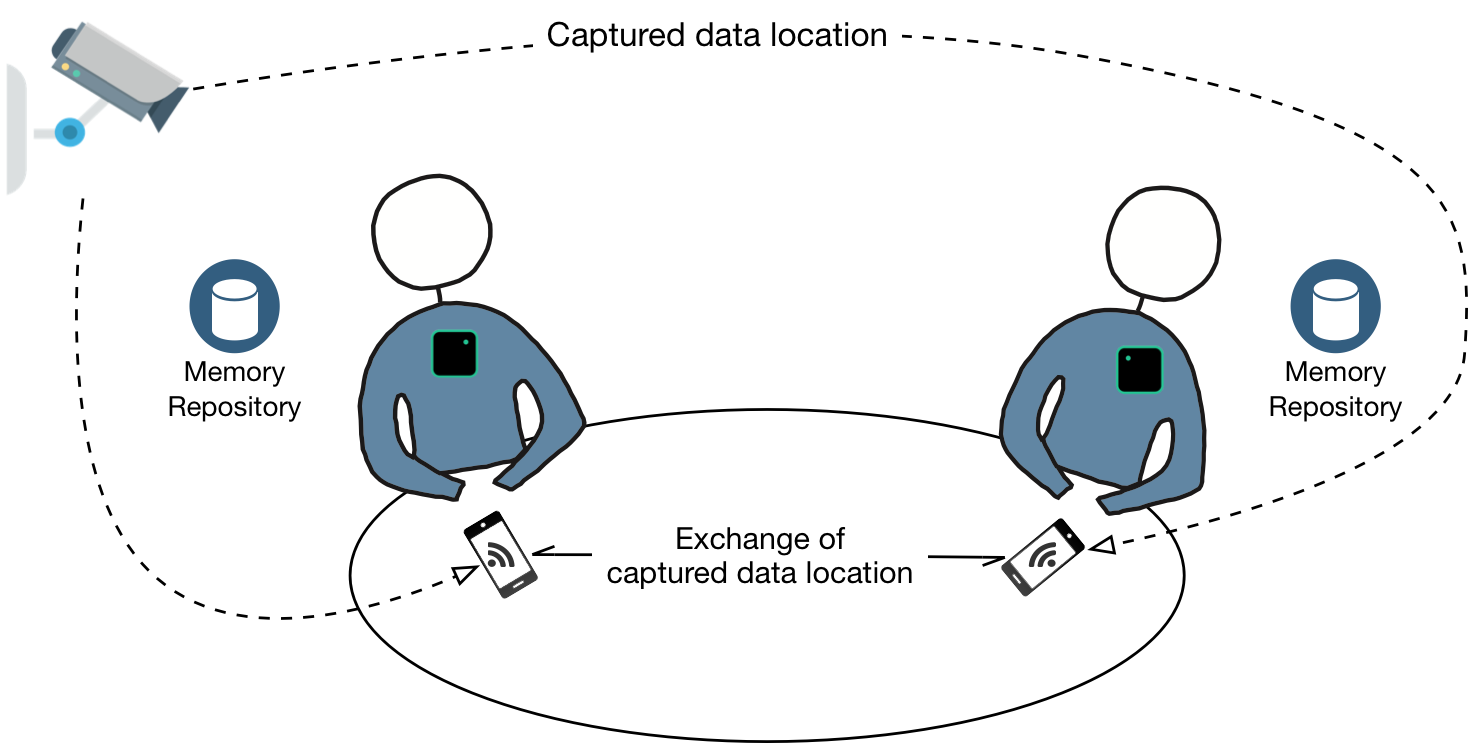
\includegraphics[width=1\textwidth]{System}
  \caption{Capturing and sharing of lifelog data between two co-located peers.}
  \label{fig2}
\end{figure}

The overall functionalities of the android application is to:
\begin{itemize}
  \item \textbf{Advertise sharing capabilities:} A device that is willing to share its data with others.
  \item \textbf{Detect peers:} When a co-located peer is detected, the device requests for secure exchange of captured data.
  \item \textbf{Secure exchange of capture data:} The device has to communicate with the co-located peer on how to securely access the images that the device has captured.
  \item \textbf{Detect end of co-location:} When the peer leaves, the system should stop sharing its captured data.
\item \textbf{Support time-limited exchange and/or Access revocation:} The system should be able to get the shared data in a limited time. 
\end{itemize}
 
From the functionalities of the android application, it is noted that the user doesn’t have much control on data capturing and sharing. For example, if the user captures and shares an image with personal information he won’t be able to withdraw or delete the shared image. For addressing the disadvantages of the initial prototype, a tangible user interface called MemStone was built to allow users to have some control over data sharing and capturing. The functionalities of this tangible user interface will be discussed in the later section \ref{sec:mem}.


\section{Objective and goals}
\label{obj}
The overall purpose of this thesis is to evaluate the components of the MemShare system to understand the usability requirements and use, to further refine the overall system. The components of the MemShare system are:
\begin{itemize}
\item \textbf{MemShare website}, this allows the user to visualize the self-captured images and the images obtained from others during an event. 
\item \textbf{MemStone} is a physical tangible device which replaced the initial prototype of the MemShare system which is an android application. 
\end{itemize}

To fulfill the purpose of this thesis, there are three main goals that should be accomplished first. The goals and objectives are:
\begin{enumerate}

\item \textbf{Designing a new web user interface for MemShare website}. A prototype website was designed as part of this thesis. Since the lifelog data captured from the MemShare system consists of large quantities of images this requires a website to effectively manage and classify the lifelog data (images). The website should also facilitate ease, rapid searching and browsing of lifelog data.

   \item \textbf{Evaluating the MemShare prototype website}. The main objective of this evaluation is to assess the overall effectiveness on how the lifelog data is presented and visualized in the prototype website. 
   \item \textbf{Evaluating MemStone device}. Only the evaluation of the MemStone device is part of this thesis. The objectives of this evaluation is to understand the strengths and weaknesses of the MemStone device. 
\end{enumerate}

By the end of this thesis, a novel website interface will be designed to visualize the captured data of the MemShare system. The website will also be evaluated by users to identify the existing usability problems and to gather feedback which can be used to further improve the website. The other component, which is the MemStone device will also be evaluated by user's. To find out its performance and how it can be improved either physical or functionally based on the collected feedback and observed use during the evaluation.

\section{Structure of the document}
This thesis is dived into six chapters. The first chapter is the introduction of the thesis, the rest are described in the following:
\begin{itemize}
\item \textbf{Chapter 2} discusses related work on how to visualize lifelog contents. Moreover, I will also present related work in usability evaluation methods for evaluating the prototype website and tangible user interface interface.
\item \textbf{Chapter 3} presents both the MemShare prototype website and the MemStone device.
\item \textbf{Chapter 4} discusses about how the MemShare website is evaluated, the methodology that I followed, as well as the the study results and feedback.
\item \textbf{Chapter 5} discusses about how the MemStone device is evaluated, the metrics and the methodology used. It also presents the result and feedback obtained from the tests.
\item \textbf{Chapter 6} concludes the thesis and discusses about the limitations and future improvements that can be made in the device and also in the website. 
\end{itemize}

\chapter{Related work}
This chapter describes the related work that have been reviewed in order to build the foundation of this thesis. One of the goals of this thesis is to create a web user interface to effectively present and visualize the lifelog contents, therefore previous work on this topic has been reviewed. This gives the direction on how to design the prototype website and what functionalities should be added to it. The main purpose of this thesis is to evaluate the MemShare system components which are the MemShare's prototype website and MemStone a tangible user interface, therefore existing evaluation methods on the Human-Computer interaction(HCI) field is reviewed to evaluate the prototype website and the device. By doing this, the different types of methods and their advantages and disadvantages are fully understood to choose a better evaluation method.     

\section{Guidelines for the presentation and visualization of lifelog content}
\label{sec:guide}

Since large amount of data is collected from lifelogging devices and most of the collected data are overlapping, this creates a problem for the user to explore and browse through it. Therefore, it is essential to organize and visualize the lifelog content effectively. According to \citeauthor{byrne_guidelines_2008}, the data should be presented in a constrained manner so that user can quickly explore into the data. In their paper, they explain that the lifelog information can be grouped together by three main axes which are people, places and time. Therefore, one of the axis can be used to group the lifelog contents and the other axis can be used to filter and manipulate the lifelog contents. They also explain that there is a higher-level concept which encapsulates these three axes together as "Events" as shown in figure \ref{fig3}.

\begin{figure}[!ht]
  \centering
  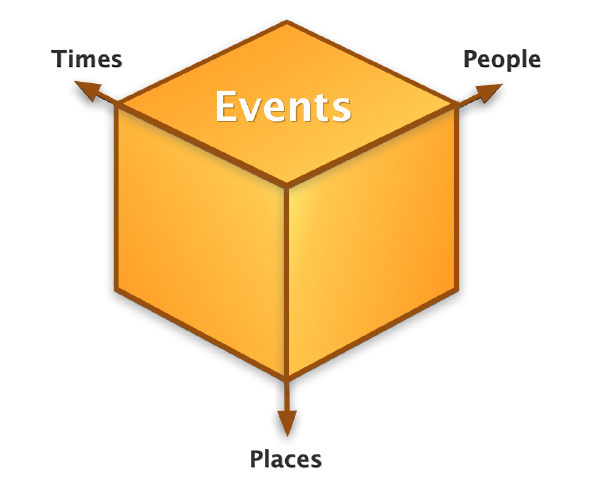
\includegraphics[width=0.5\textwidth]{Events}
  \caption{Representation of the three axes of a lifelog by \citeauthor{byrne_guidelines_2008}}
  \label{fig3}
\end{figure}

An event is defined as series of grouped temporal related items. It is important to group the lifelog data into segments which reduces the visualization complexity problem for the user \citep{yang_visualizing_2013}. These events can be made up of different visualization tools such as calendar and timeline.
\linebreak

The paper \citep{byrne_guidelines_2008}, also gives some design goals that should be taken into consideration while presenting and visualizing the lifelog content.

\begin{itemize}
\item \textbf{Simple and Intuitive Interface:} Since the potential users range from different age groups the interface should be simple which enables quick and easy access to their lifelog contents. Exploring and navigating between contents should be simple and the contents should be displayed in an intuitive manner. 
\item \textbf{Manage and reduce large lifelog data into comprehensible units:} As mentioned before, the lifelog contents should be grouped into events.
\item \textbf{Aid human memory:} The visualization of the lifelog contents should intend to help the users to recall their past experiences.
\item \textbf{Allow for exploration and comparison:} The interface should enable quick exploration through the collection of lifelog contents and provide an effective summary of the content so that this will allow the user to compare different events.
\item \textbf{Enjoyable, rich and engaging but also meaningful:} The interface should have enjoyable but also meaningful visualizations such as animations or transitions.  
\end{itemize}

According to \citeauthor{teraoka_organization_2012}, the effective way to visualize the data is to have an organized structure and a zooming user interface for the exploration of the content. In our case, the organized structure can be events which can be zoomed into people and then the shared images captured by the lifelog device. 
\newline

By keeping these concepts and design goals in mind, a web user interface was created. The design and functionalities of this interface is presented on chapter \ref{sec:web}. On this interface, users can organize and visualize the contents from the MemShare system which helps to recall and reminisce about their past experiences. It also allows them to explore their own personal data as well as personal data from co-located people.

\section{Evaluation methods for website prototypes}

There are many methods for evaluating a prototype website but the evaluation method which involves with actual users to evaluate a product is known as usability evaluation. It is one of the techniques of Human-Computer interaction (HCI) field which aims to improve the usability of computer interfaces by testing out with users. Before we talk about the usability evaluation methods, we should know what exactly "usability" means. According to ISO 9241-11 usability is, "The degree to which a product can be used by specific users to reach specific goals with efficiency, effectiveness and satisfaction in a given use context" \cite{smith_iso_1996}. From this definition, it is known that usability can be measured from the three dimensions which are effectiveness, efficiency and satisfaction. Moreover, from the definition it is also noted that only one dimension measure is not a sufficient indicator for overall usability.

There is a wide range of usability evaluation methods that can be used at different stages of development of the website. Some of these evaluation methods get data from users and the rest rely on experts. Here are some of the usability evaluation methods, which are heuristic evaluation, usability testing and focus group. 
\newline

\textbf{Heuristics evaluation/Expert review:}
This type of method is categorized as an inspection method were evaluators inspect the interface using usability principles or heuristics. This method is performed without involving actual users. According to \citep{fu_effectiveness_2002} this method only uncovers expert user usability problems and it is not effective to identify novice users usability problems. 
\newline

\textbf{Usability testing:}
This method involves in letting actual users to interact with the product or system and observing them. In this method, user will be placed in a realistic environment and the evaluator will give a set of tasks to the user to perform with the product or system. The experiment will usually be video recorded to measure user's performance such as task success, task completion time, task errors and to observe user's interaction with the product. By analyzing the data from the experiment, we can find out the usability problems faced by the user.
\newline

\textbf{Focus groups: }
This method is an inquiry type which can be very useful in the early phase of the project to understand the end user's needs. A moderator will lead a discussion with a group of potential users and he will note down the points discussed. This will be used in the further development of the product.
\newline

By comparing the three evaluation methods, usability testing is chosen for evaluating the prototype website since it involves in actual users interacting with the prototype and from the evaluation the usability problems can be identified which can further improve the design of the website. Now it is important to know what type of usability testing should be used. The type of usability testing differs by what research questions was defined, what development phase the product is in, and time available \cite{rubin_handbook_2008}. Figure \ref{fig4} shows the different type of usability testing.

\begin{figure}[!ht]
  \centering
  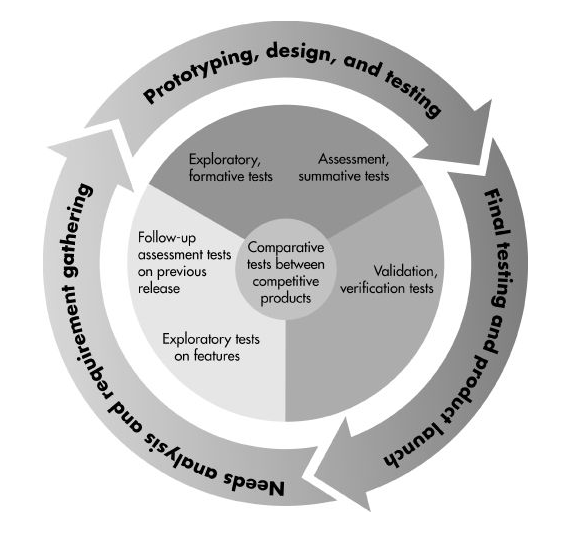
\includegraphics[width=0.5\textwidth]{cycle}
  \caption{Usability testing throughout the product lifecycle; source: \cite{rubin_handbook_2008}.}
  \label{fig4}
\end{figure}

There are four types of usability testing methods formative (exploratory), summative (assessment), verification(validity) and comparison test.

\begin{itemize}
\item \textbf{Formative test:} This type of usability test is done in the preliminary stages of product development where it is designed. The objective of this study is to examine the effectiveness of the design.
\item \textbf{Summative test}: This type of test is simple and very direct to conduct. The purpose of this test is to further investigate the findings from formative test. This test is performed in the early or middle stages of the product development.
\item \textbf{Verification test:} This test is usually conducted in the late cycle of product development. This test is used to compare the product with a predefined benchmark 
\item \textbf{Comparison test:} This test can be used at any stage of the product development cycle. In this test, two versions of the product are tested to figure out which one is better. 
\end{itemize}

The evaluation method chosen for evaluating the MemShare prototype website is usability testing because it is the best way to understand how users works with the interface or system by observing. The collected data and gathered feedback from the user will be useful to identify the usability problems faced by the user during the experiment. The type of usability testing that will be used during the evaluation of the MemShare prototype website will be a formative test since it is suitable for evaluating prototype interfaces. 

\section{Evaluation methods for tangible user interfaces(TUI)}
There is no specific evaluation method that have been devised for evaluating tangible user interfaces (TUI's) because it is a very novel field \citep{shaer_tangible_2009}. Since there is no specific evaluation method, this section discusses mostly on the previous conducted studies on how evaluation is done on different tangible devices. This gives an idea on how to evaluate the MemStone device. From previous studies the evaluation method used for evaluating tangible user interfaces are similar to the evaluation methods existing in the Human-Computer interaction(HCI) field and the type of evaluation method used in previous studies are mostly either comparative studies or qualitative observation studies.
\newline

\textbf{Comparative studies:}

These studies were mostly involving in heuristics evaluation or empirical lab evaluation. In these studies, the tangible user interface is often compared with different versions of the tangible user interfaces or with a graphical user interface (GUI). In some of the studies for evaluating TUI's, other than the traditional performance metric such as errors, task completion time and task success measured during the evaluation also subjective data (Such as collaboration, engagement, enjoyment and so on) were collected by questionnaires in the end of the study. This can be seen in the study done by \citeauthor{parmar_tangible_2009}, where an health information system TUI was evaluated against an iconic keyboard interface system with a group of 175 women. After the evaluation the participants were asked to rate the systems in terms of social interaction and engagement. The subjective data is gathered because to understand the quality of the interaction done on the tangible device. For example, if the tangible device involves in two or more user's interaction then the subjective data collaboration is measured.
\newline

\textbf{Qualitative observation studies:}

These studies were mostly based on ethnographic observations and interaction analysis. The ethnographic observation studies involve user's using the tangible device in their natural environment rather than in lab. In these studies, the researcher observes and notes down how the participant interacts with the device in his natural environment. Other than the qualitative observation, interviews were also taken in some studies. The interviews were transcribed and the qualitative data is analyzed to find description about important aspects or problems. Using these detailed descriptions a hypothesis can be developed that can be later tested with an experimental study. Interaction analysis is an interdisciplinary method in which interactions with human beings or with objects in an environment is investigated \citep{jordan_interaction_1995}. The studies which uses the interaction method involves in analyzing video's for observing verbal and non-verbal behaviors while the user interacts with products. The study done by \citeauthor{ryokai_i/o_2004}, used interaction analysis method to analyze the video captured during the evaluation of a augmented painting tool interacted by children's at a kindergarten. In his study he observed children's interaction with the TUI for studying children's creativity. 
\newline

For evaluating the MemStone device, usability testing method is chosen and the type of evaluation method will be a comparative study where the device is compared with an smartphone user interface. This method was chosen because the MemStone device was created to replaces the existing android application to provide better control and hence a comparative study is a suitable for evaluating MemStone device. The smartphone application is an another version of MemStone device, which was created to serve as a benchmark for evaluating the MemStone device by comparing the performance measures and other interaction quality measures between them to find out the best interface for the MemShare system. The smartphone application functionalities and design will be presented in section \ref{sec:smrt}. At the end of the comparative study qualitative data will also be collected through interviews and the data will be analyzed to form hypothesis which will be supported by the evaluation.  

\chapter{Components of the MemShare system}
\label{sec:bot}
In this chapter, the components of the MemShare system are presented which are MemStone device and the MemShare website. A new web user interface was designed for the MemShare website as a prototype and this chapter presents the web user interface of the MemShare's prototype website. In more detail the visual design, functionalities and the steps taken to design the prototype will be discussed in this chapter. For evaluating the MemStone tangible interface, a smartphone user interface was designed which acts as a baseline to compare between these two interfaces. The functionalities of MemStone device and smartphone application will also be discussed in this chapter. 

\section{MemShare prototype website design}
\label{sec:web}
As mentioned before, one of the goals of this thesis is to design a new web user interface for visualizing and presenting the huge archive of lifelog data in an effective way, so that when the user goes through these lifelog contents it would help him to remember his past memories by giving cues. The following section explains the initial requirements needed to design the prototype website, the website structure and functionalities are presented in subsequent sections.  

\subsection{Requirements}
To understand user requirements for the website, scenarios were considered to discover the requirements on how users expect and how they will interact with the content, the features and functions of the website. These are the following scenario which were considered:

\begin{itemize}
\item \textbf{After a work meeting:}
User should be able to see who are participants of the meeting and at what time they arrived and left the meeting. 
\item \textbf{Exploring the captured photos:}
User should be able to access the images shared by each co-located participant and all the images captured and shared during the meeting. The shared images should have details about who captured the image and at what time it is been captured.
\item \textbf{Important information shared during the meeting:}
User should be able to annotate the captured image or mark it as his favorite to easily identify it in the future.
\item \textbf{Recalling the important information shared during the meeting:}
User should be able to search and find the image which he had annotated before and user should be able to view all his favorite images. 
\item \textbf{Recalling an event that happened 2 weeks ago:}
User should be able to search and find an event (meeting) by date. 
\item \textbf{Recalling events that happened in the office:}
User should be able to sort the list of events in the website by location.
\end{itemize}

These are the initial requirements that were identified in the early stages of designing the prototype website and this served as a starting point. During the evaluation of the prototype more requirements will be collected and the usability problems will be identified.

\subsection{High fidelity prototyping}

Instead of using low fidelity prototype like wire-frames or paper prototypes to design the prototype website, a high fidelity functional prototype website was designed using a prototyping tool called "JustInMind"\footnote{\url{https://www.justinmind.com}}. The prototype website was designed based on the concepts and design goals which were discussed in section \ref{sec:guide}. Some of these design goals suggested transition and animation effects to be used in the interface to make it more enjoyable and engaging experience to the user. Therefore, this gives the reason to use a functional prototype. 

\subsection{Site structure}

This section will present how the prototype site is structured, how the contents are organized and design of the prototype website. 

The prototype website has a home page that is displayed after a user logs in and the home page has a list of all events related to the user as shown in figure \ref{fig5}. These events are comprised of lifelog data that has been acquired by user's MemShare system. Each of these events are made up of the lifelog data that has been captured by user and the lifelog data that has been shared with user from co-located peers. An event is recorded by the site only when user starts capturing and sharing the lifelog data and the event ends when user stops capturing.

\begin{figure}[!ht]
  \centering
  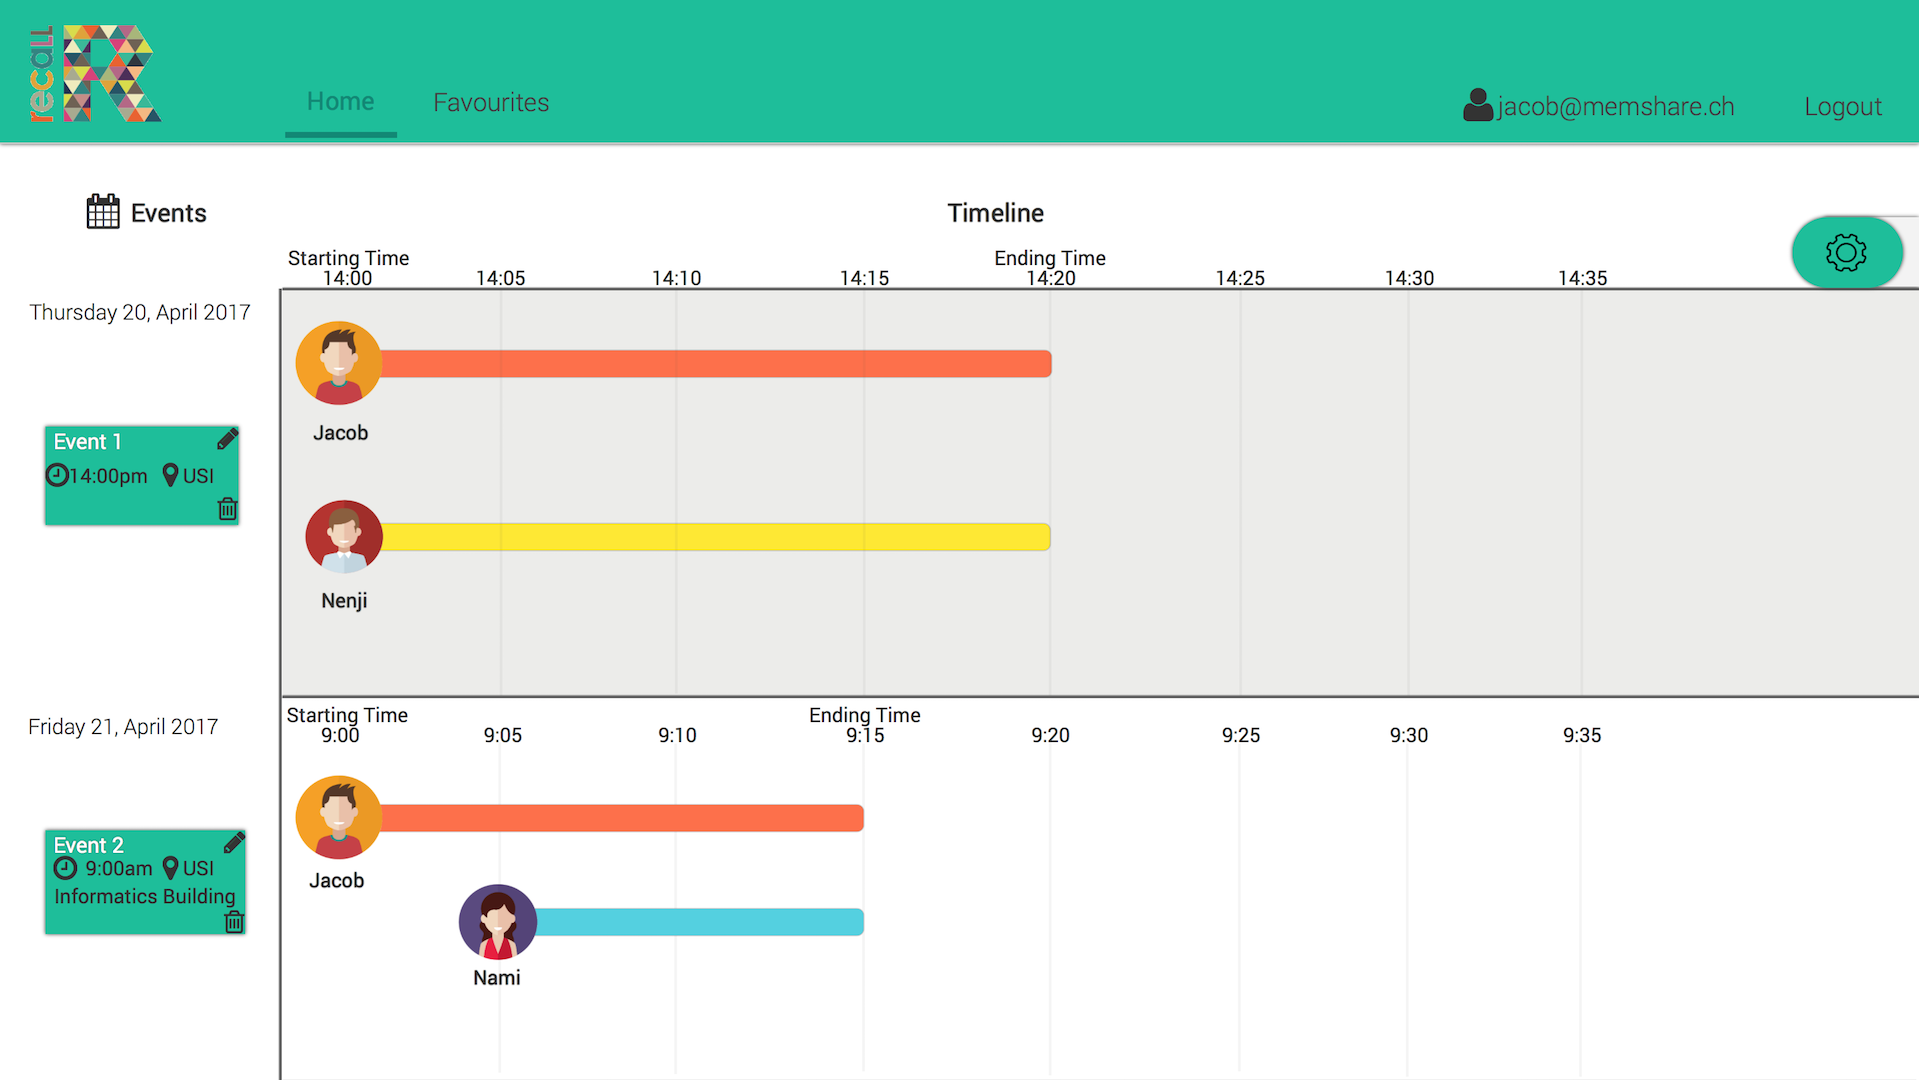
\includegraphics[width=1\textwidth]{Home}
  \caption{Homepage of MemShare's prototype website.}
  \label{fig5}
\end{figure}

On the left-hand side of the homepage, each event's information is displayed such as the date of occurrence, the location and the starting time of the event. These events are automatically named sequentially by the site and the user can rename it. There is also an option to delete an event from the site. 

To show more information about events in the prototype in a simple and intuitive way, a timeline like interface is adopted. The timeline interface shows when an event started and ended which means when the user starts capturing and stops capturing. It also shows the participants or peers of the event, which is represented by a circular avatar and below it the name of the participant is presented. The logged in user's avatar is displayed in the first position of each event and if there are any co-located peers present with the user their avatar is shown below. Besides every people (user and peers) avatar there is a timeflow bar which denotes when they started to capture and share lifelog data and when they stopped. For example, in figure \ref{fig5} on Event 2 user Jacob starts to capture from 9:00 and stops at 9:15. But the other co-located peer arrives and starts capturing on 9:05. At 9:15 the co-located peers stop and leaves the event. By comprising the lifelog data into events will allow user to easily manage and explore the contents.

\begin{figure}[!ht]
  \centering
  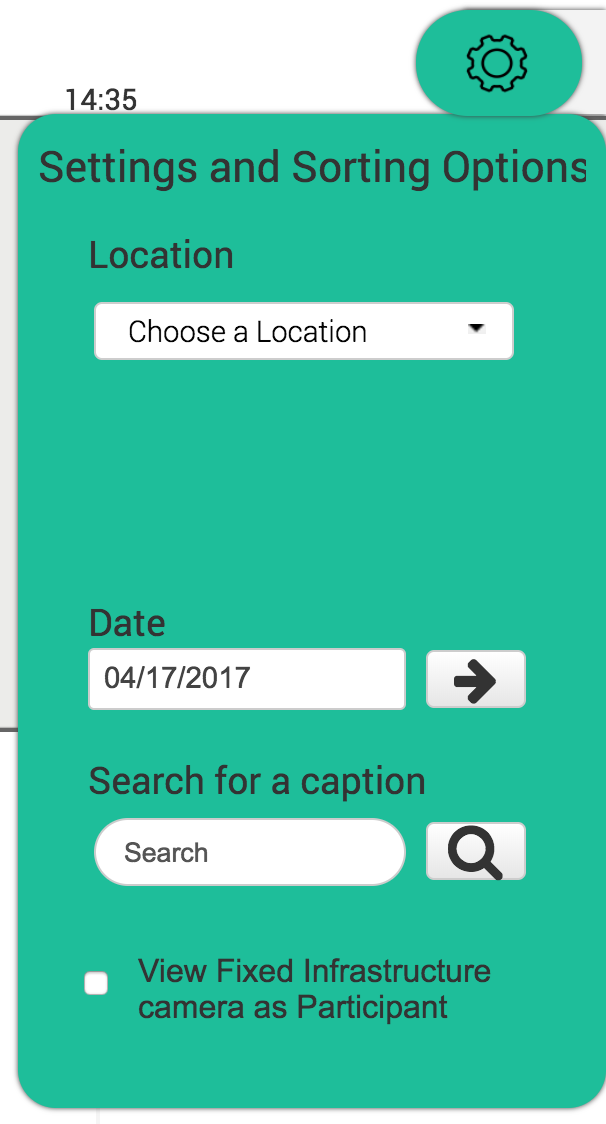
\includegraphics[width=0.3\textwidth]{Sort}
  \caption{Settings and sorting options menu.}
  \label{fig6}
\end{figure}

On the right side of the home page there is an click-able option with a settings wheel icon. When the user interacts with it by clicking, a hidden slide menu pops out showing the settings and sorting options as shown in figure \ref{fig6}. This menu contains the sorting options to sort the events in the home page. Using this menu, the events can be sorted by date and location. This will allow the user to quickly explore the events and to compare different events. If the homepage is filled with events and the user want to find a specific event, instead of scrolling through the whole home page users can use these options. The menu also contains a search function to search and find an annotated image which is either captured by the user or shared by the co-located peers. This allows users to search and find the information quickly. The last option in the menu is for enabling the infrastructure camera as a participant, this option is included because the MemShare system also captures the images from any nearby infrastructure camera since these images have a full perspective of the event. 

\begin{figure}[!ht]
  \centering
  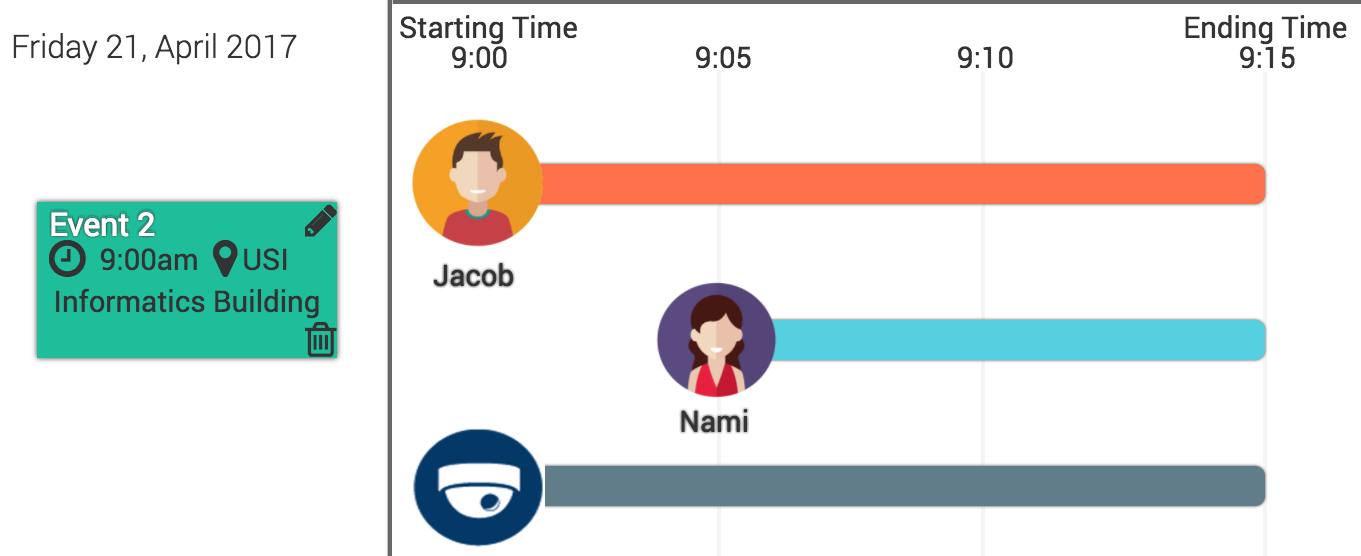
\includegraphics[width=0.7\textwidth]{Infra}
  \caption{Infrastructure camera as a participant.}
  \label{fig7}
\end{figure}

By enabling this option, if there is an infrastructure camera present during the event then the avatar of the camera appears in the timeline as shown in figure \ref{fig7} for Event 2. The infrastructure camera avatar is hidden initially because some prefer not to see the infrastructure camera as a participant, then it can be enabled in the settings and sorting options menu.

\begin{figure} [!ht]
\begin{subfigure}{0.4\textwidth}
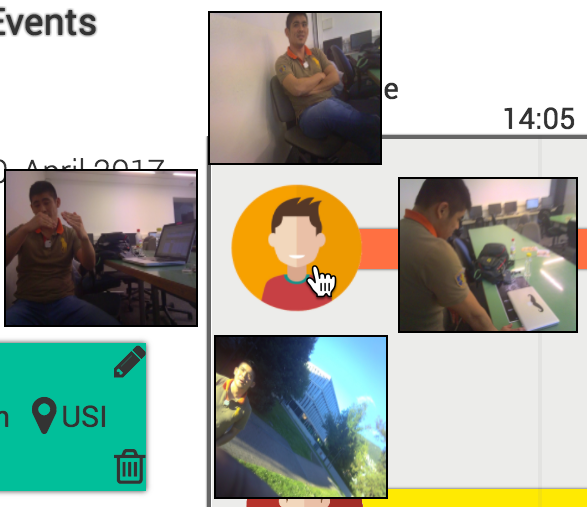
\includegraphics[width=\linewidth]{Hover1}
\caption{Transition effect for individual's avatar.} \label{fig8}
\end{subfigure}
\hspace*{\fill} % separation between the subfigures
\begin{subfigure}{0.55\textwidth}
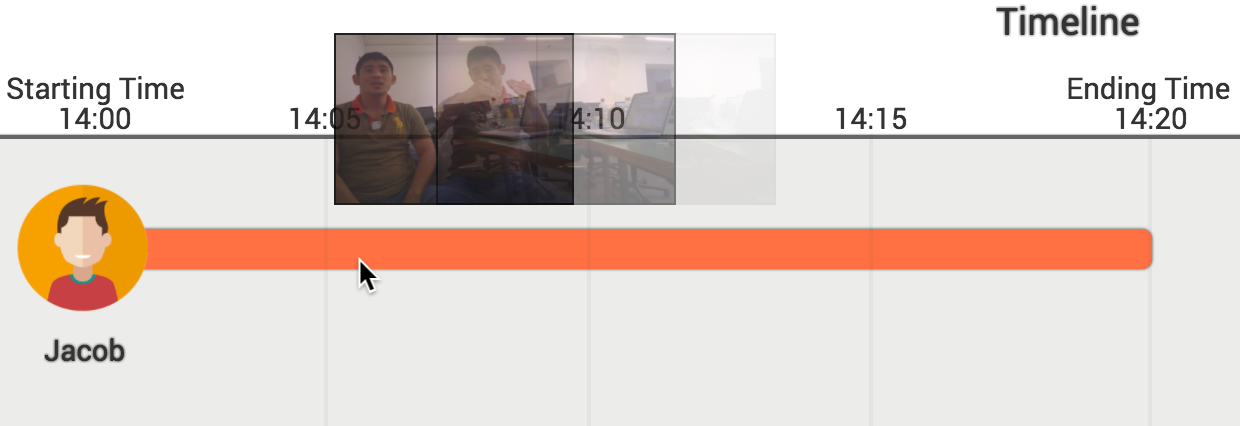
\includegraphics[width=\linewidth]{Hover2}
\caption{Transition effect on timeflow bar.} \label{fig9}
\end{subfigure}
\caption{Available transition effects in the prototype website.} \label{fig10}
\end{figure}

To make the user's experience more enjoyable and engaging some visual transition effects were added to the prototype. When the user hovers over the timeflow bar in the timeline, images are displayed corresponding to the time when it is captured either by user or peer as shown in figure \ref{fig9}. Another transition effect is that, when the user hovers over the avatar's which is present in the timeline, it shows four relevant pictures captured by participant or user as shown in figure \ref{fig8}. These transition effects give a summary or overview of the events to compare with different events.

\begin{figure}[!ht]
  \centering
  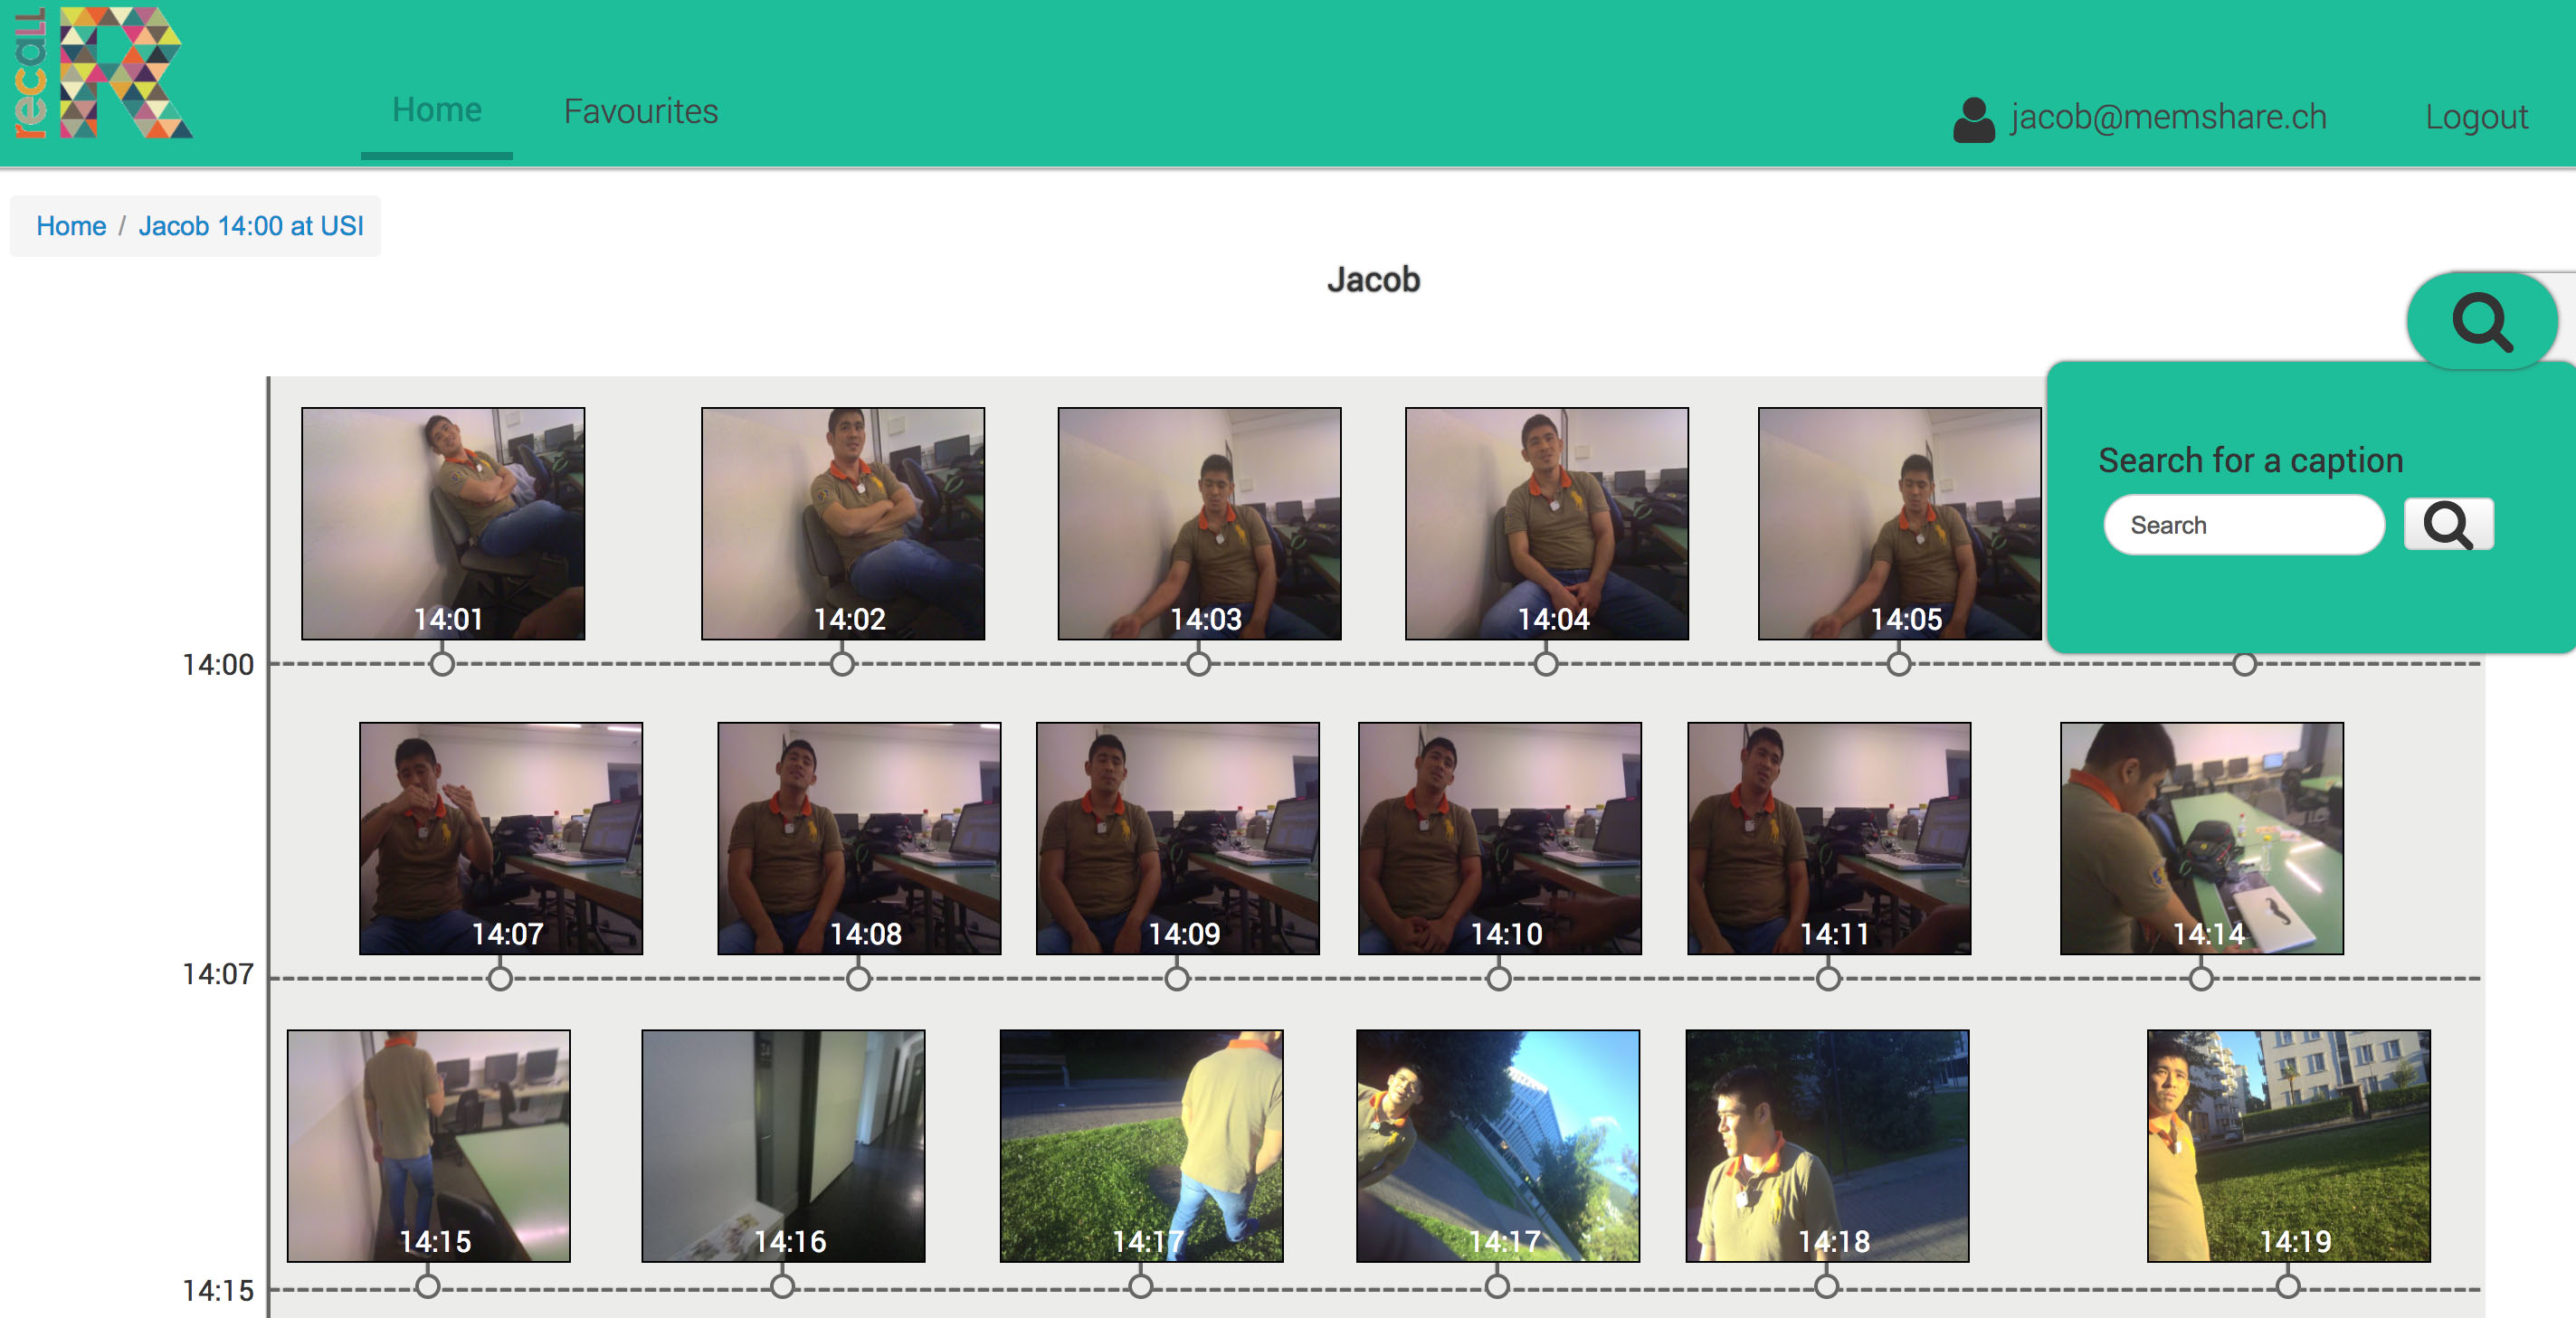
\includegraphics[width=0.9\textwidth]{User}
  \caption{Individuals page with captured images.}
  \label{fig11}
\end{figure}

For visualizing all the images captured by an individual (can be user or peer), user can click on the individual's avatar displayed on the timeline of the home page. This action opens another page where all the images captured by the individual during an event is displayed as shown in figure \ref{fig11}. The thumbnails of the images are placed in a horizontal way on a timeline like interface. On the bottom of each image thumbnail the time on which the image was taken is displayed. 

\begin{figure}[!ht]
  \centering
  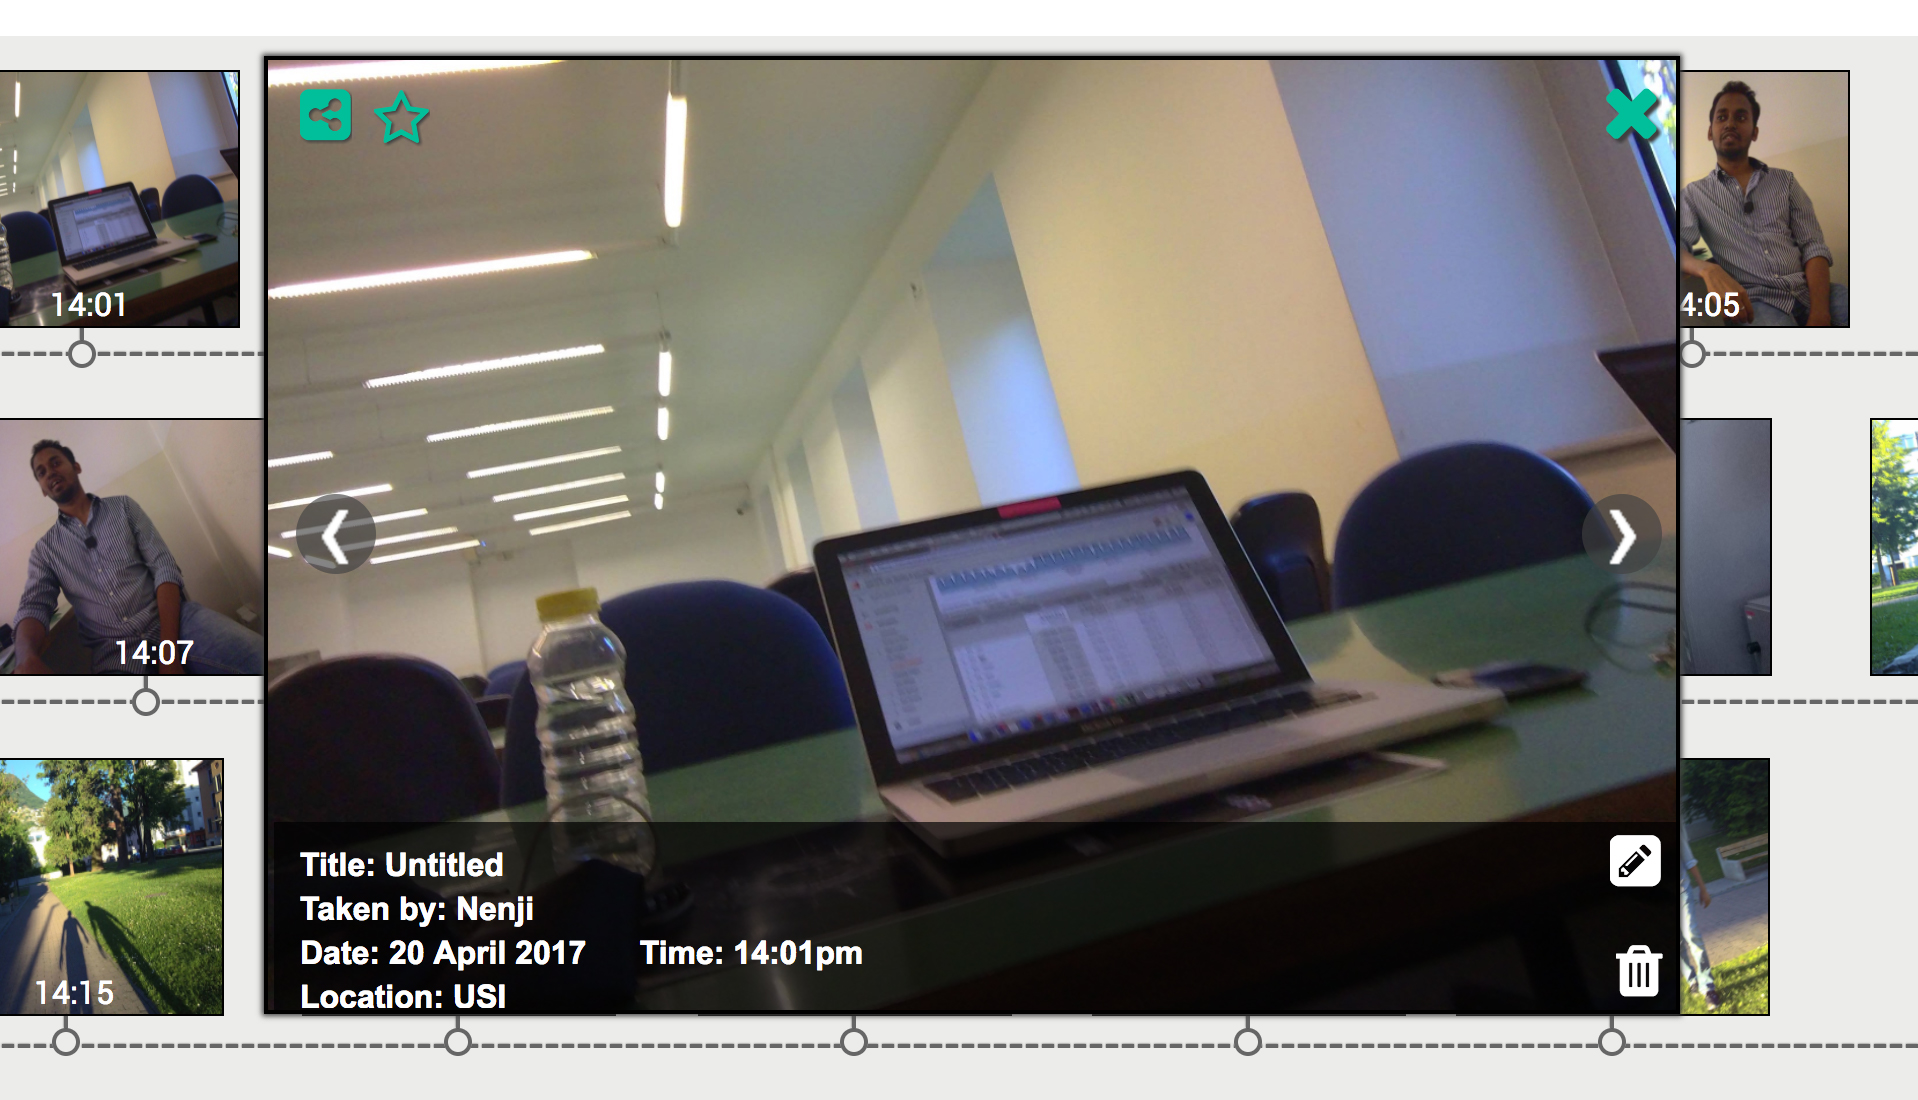
\includegraphics[width=0.7\textwidth]{Pop}
  \caption{Image details window.}
  \label{fig12}
\end{figure}

Any image thumbnail present in the individual's page can be clicked and zoomed in to have a better view of the image. This pops up a window containing the image and in the bottom of the window the details about the image is also displayed as shown in figure \ref{fig12}. Details such as, when it was captured, the location, the author of the image and a title for the image. Initially the title of the image will be set to untitled and the user can set the title using the edit option. The pop up window also has icons which does the following actions such as favorite icon to mark the image as favorites and it can be viewed later in the favorites page, it has a sharing option icon to share the image in email or social media, a set of direction icons to view the next or previous images, a delete option to delete the zoomed in image and a close option to close the pop up window. 

On the right side of the individual's page there is a intractable option with a search icon, when it is interacted a search bar appears as shown in figure \ref{fig11}. By using this search bar user can find the annotated image from the event. This option will be useful for searching for an important image in the vast contents of captured data. 

\begin{figure}[!ht]
  \centering
  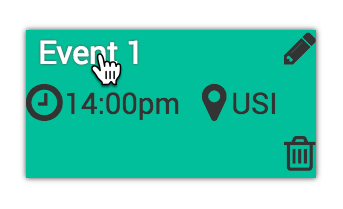
\includegraphics[width=0.27\textwidth]{EventLabel}
  \caption{Event Label}
  \label{fig13}
\end{figure}

For visualizing all the images captured during an event, both personally and shared one's from co-located peer, the user can access them by clicking on the event label which is present on the left side of the home page as shown in figure \ref{fig13}. This will open a new page where user can see all the pictures captured and shared during the event. In this page, the images thumbnails are ordered according to when they are captured by the individual and the time when it was taken is also displayed in the image thumbnail as shown in figure \ref{fig14}.

\begin{figure}[!ht]
  \centering
  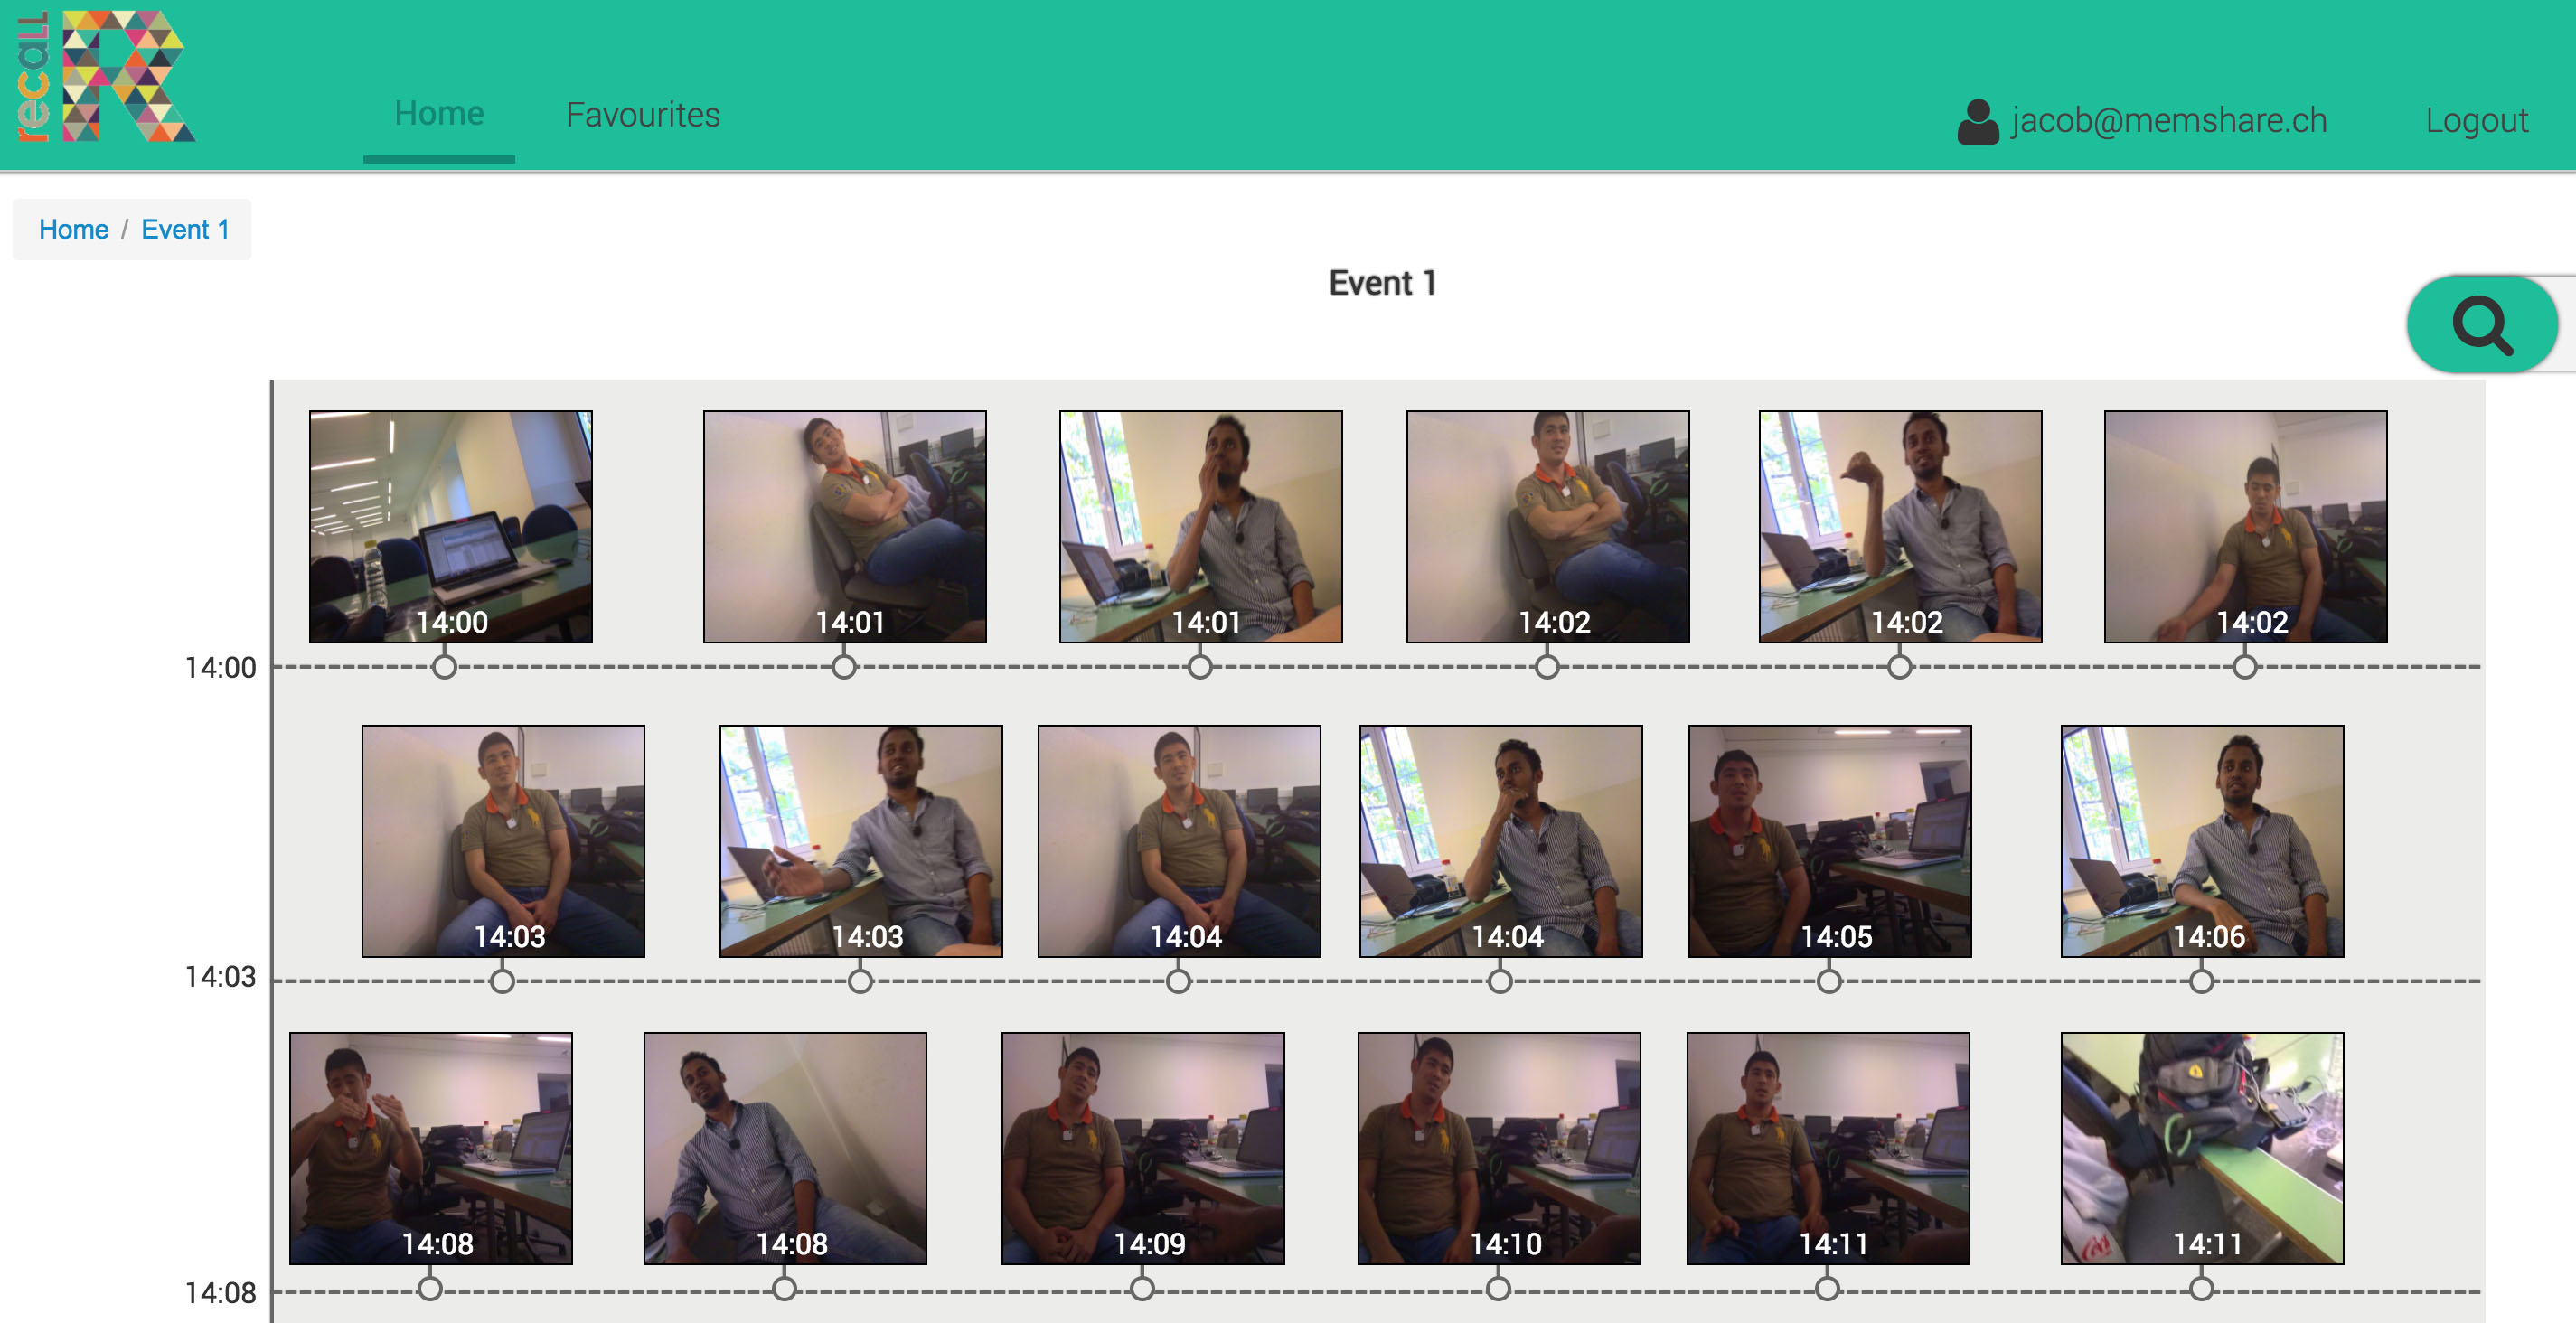
\includegraphics[width=0.9\textwidth]{EventPage}
  \caption{Event Page with all captured and shared images.}
  \label{fig14}
\end{figure}

\section{MemStone}
\label{sec:mem}
This section will present the MemStone tangible user interface which was built to overcome the drawbacks of the previous prototype of MemShare system, which lacks in control to make sharing and capturing decisions. Other than the MemStone tangible interface, an smartphone user interface was designed which has the same functionalities of the MemStone tangible interface. This smartphone user interface was built for evaluating with the MemStone device, to compare both of them and to find out the strengths and weaknesses of the MemStone device. 

\subsection{MemStone tangible interface}

The MemShare system was implemented in an tangible device which was built with an Aurdino micro-controller and sensors. In this section, the architecture of the device wont be discussed since its not a part of this thesis, only the functions of the device will be presented in this section. The device was built in order to act as a controller to allow the user for making data capture and data sharing decisions using built-in gestures.

\begin{figure}[!ht]
  \centering
  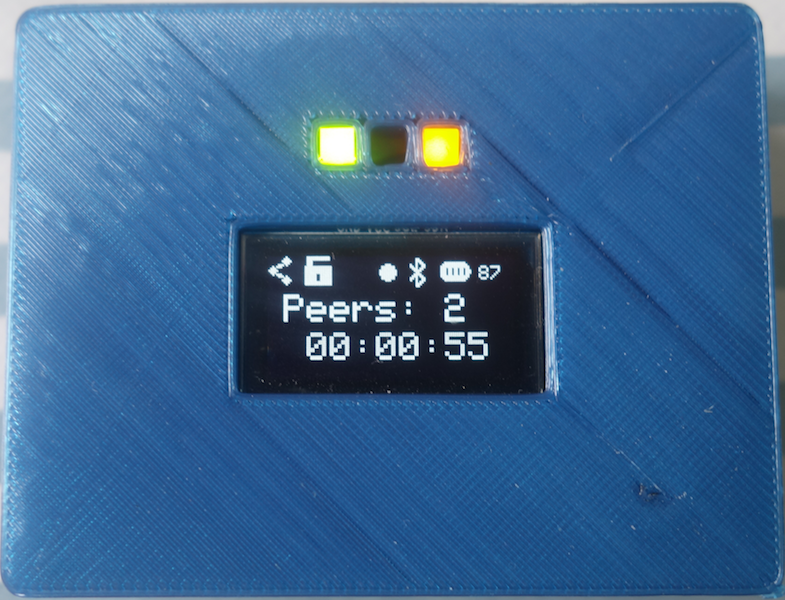
\includegraphics[width=0.40\textwidth]{MemStone}
  \caption{MemStone device.}
  \label{fig15}
\end{figure}

Figure \ref{fig3} shows how the MemStone device looks like. This device is still in the prototype phase so that not all the functionalities are implement into the device. The MemStone device has 2 LED's with different colors, one is to denote whether the device is recording or not and the another is to inform the user whether it is sharing the captured data with other co-located peers or not. In the middle of the device there is a small screen to show information such as elapsed time since sharing, number of sharing peers and other icons such as lock, battery. There are five gestures present in the MemStone device to control data sharing and capturing decisions. And whenever a gesture is performed, the device will give a vibration feedback to notify the user that a gesture has been performed and also shows the revelant information in the screen. These are the gestures present in the MemStone device as shown in figure \ref{fig:1}:

\begin{figure} [!ht]
\begin{subfigure}{0.19\textwidth}
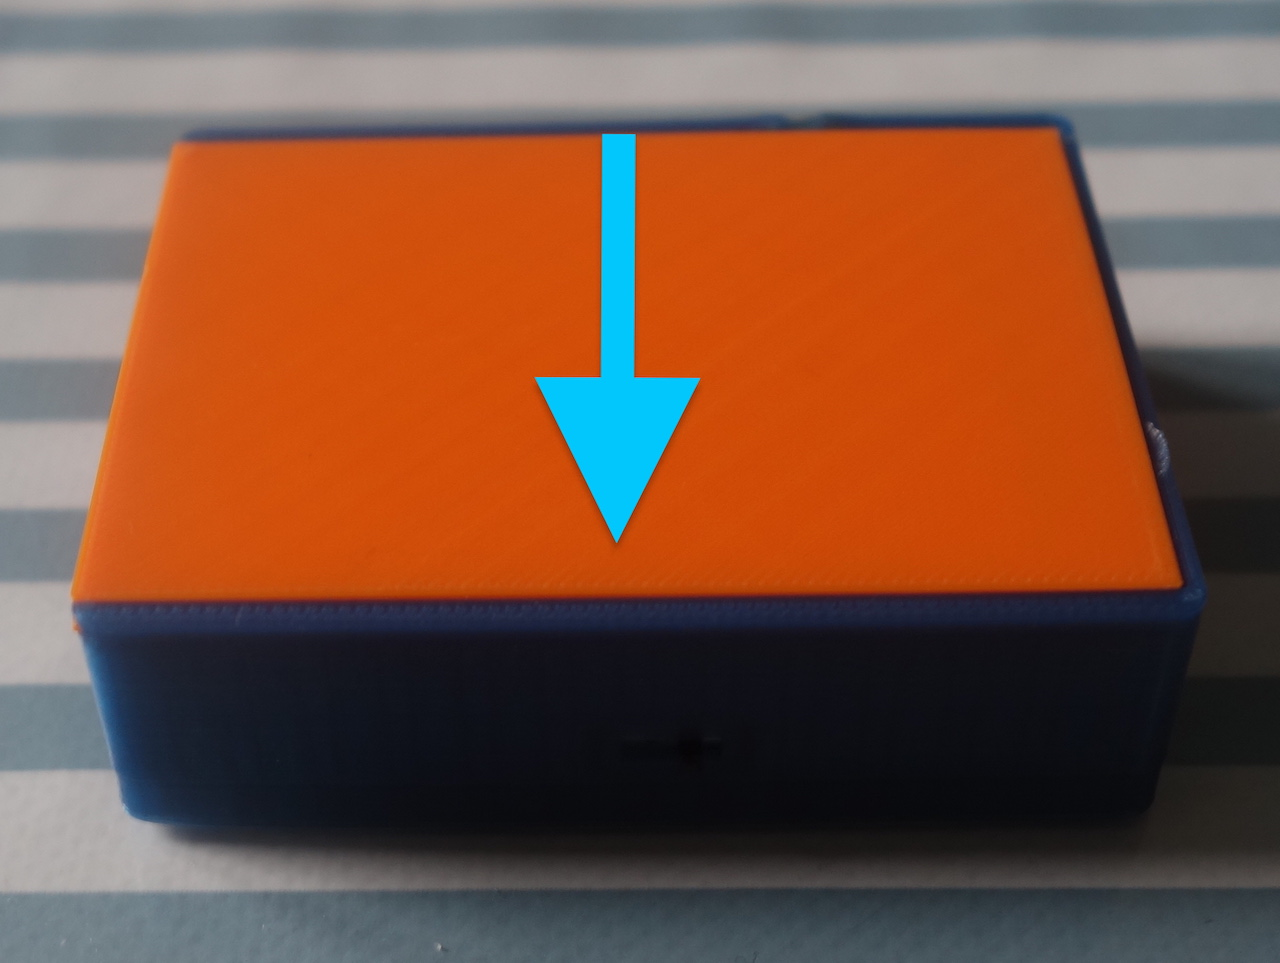
\includegraphics[width=\linewidth]{Facedown}
\caption{Face down} \label{fig:1a}
\end{subfigure}
\hspace*{\fill} % separation between the subfigures
\begin{subfigure}{0.19\textwidth}
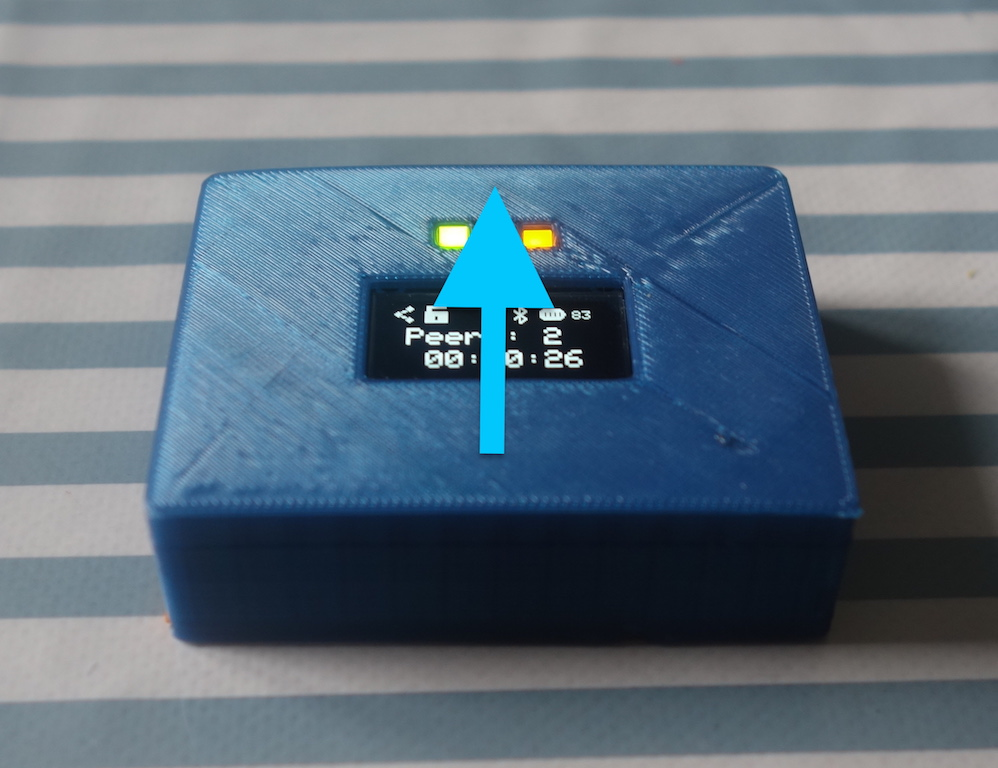
\includegraphics[width=\linewidth]{Faceup}
\caption{Face up} \label{fig:1b}
\end{subfigure}
\hspace*{\fill} % separation between the subfigures
\begin{subfigure}{0.20\textwidth}
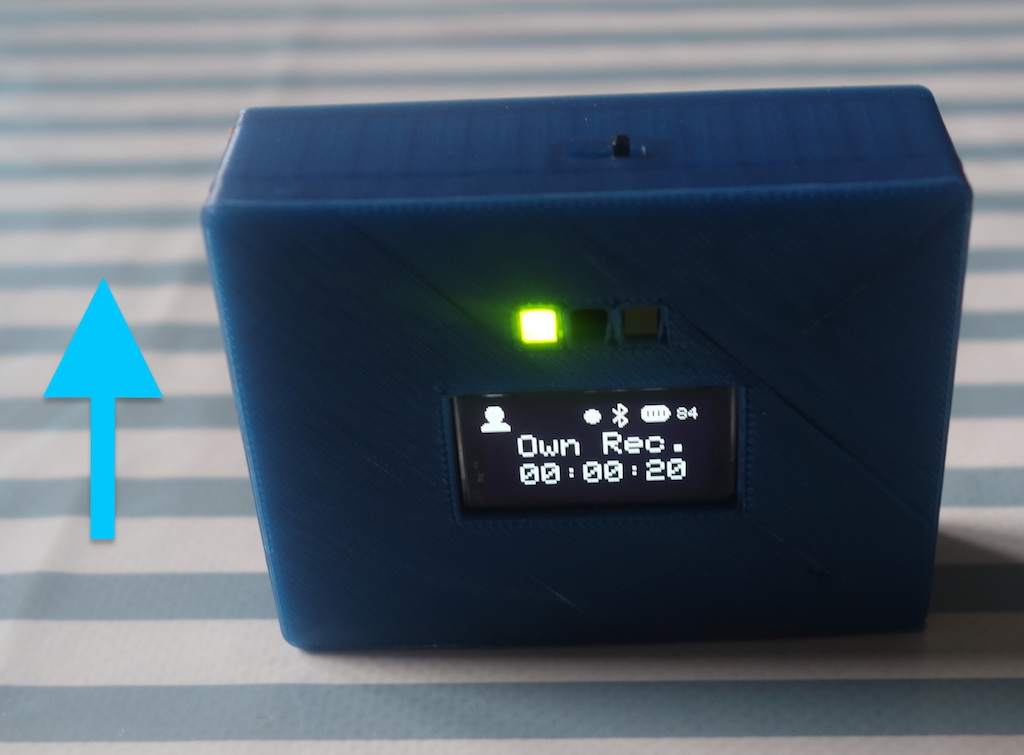
\includegraphics[width=\linewidth]{Vertical}
\caption{Vertical} \label{fig:1c}
\end{subfigure}
\hspace*{\fill} % separation between the subfigures
\begin{subfigure}{0.20\textwidth}
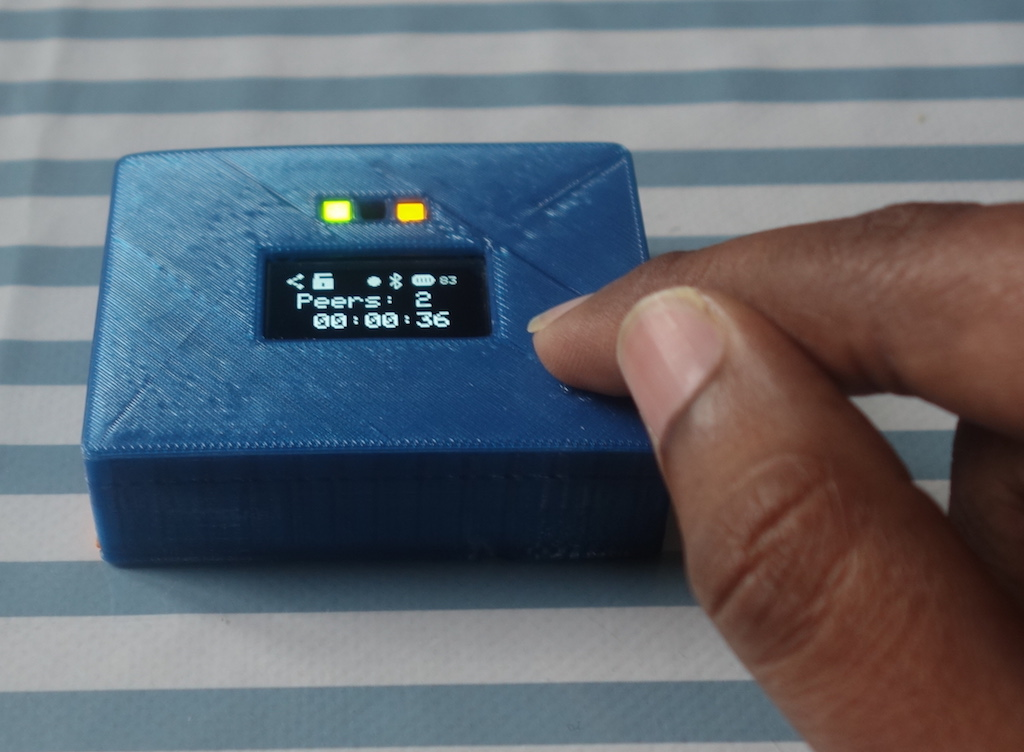
\includegraphics[width=\linewidth]{Doubletap}
\caption{Double tap} \label{fig:1d}
\end{subfigure}
\hspace*{\fill} % separation between the subfigures
\begin{subfigure}{0.16\textwidth}
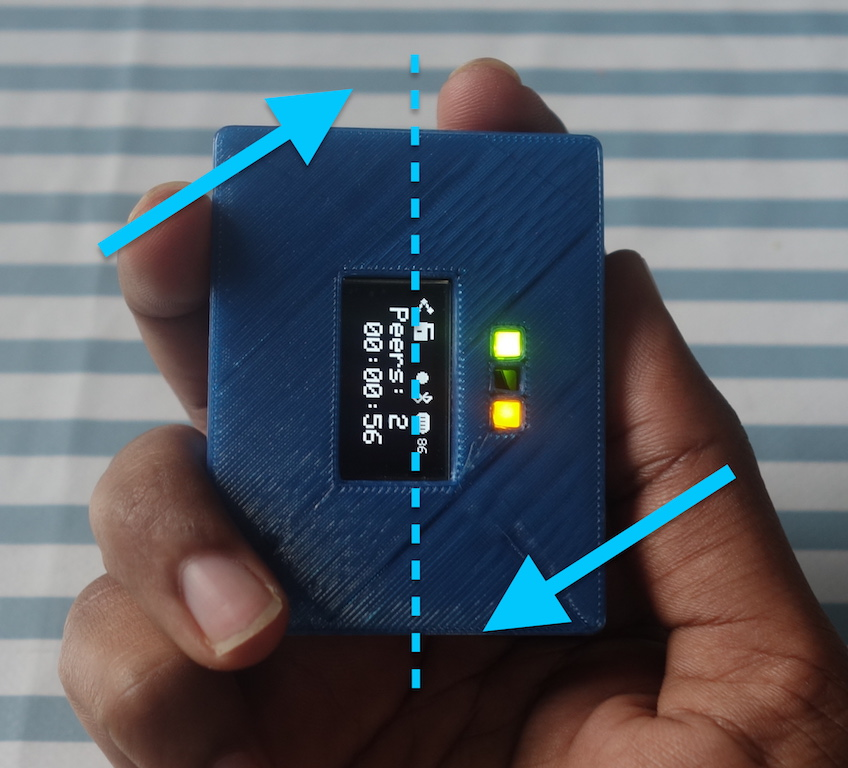
\includegraphics[width=\linewidth]{Shake}
\caption{Shake} \label{fig:1e}
\end{subfigure}
\caption{Available gestures in the MemStone device.} \label{fig:1}
\end{figure}
\begin{itemize}
  \item Face-Down Gesture: This gesture stops both data capture (sourced from any of the user's capture devices) and data sharing with other co-located people. For example, this gesture can be used in the situation when the user doesn't want to record nor share in a meeting. After performing this gesture the screen displays no recording text and both the LED's will be off. 
  \item Face-Up Gesture: This gesture triggers data capture again from the capturing device and sharing will automatically commence with other co-located people. For example, after the face-down gesture a user can do face up to resume data capturing and sharing in a meeting. After performing this gesture the screen displays the number of peers its sharing with, a small sharing icon will be displyed in the left corner of the screen and also a timer will get started which shows the elapsed time since recording and sharing started. 
  \item Vertical Face-Up Gesture: This gesture is used for own recording. By activating this gesture, you will capture only for yourself and you won't share the capture data with other peers. For example, this gesture can be used when the user is working alone and he/she wants to capture only from his/her capturing device. After performing this gesture the number of peers wont be displayed instead the screen displays the text own recording and also a profile icon is displayed at the left corner of the screen instead of the sharing icon.
  \item Double Tap Gesture: This gesture "locks" the data exchange with the current set of co-located people and prevents any further peers from joining. A subsequent double tap will remove this lock. For example, this gesture can be used to prevent strangers from joining a meeting. After performing this gesture a lock icon is displayed in the right corner of the screen. 
  \item Shake Gesture: This gesture is used for deleting the last 30 seconds of the captured data so that the shared data to the co-located peer will also be deleted. This gesture will be handy in a situation where you accidentally capture some sensitive information and you can delete the captured and shared image. After performing this gesture the screen displays the text that last 30 seconds has been deleted.
\end{itemize}

\subsection{Smartphone application}
\label{sec:smrt}
The smartphone application was designed only to evaluate the MemStone tangible device by comparing both of them with users and the smartphone application acts as a baseline for comparison. The smartphone application has a very simple design with few buttons which replaces the MemStone device gestures to control data sharing and data recording preferences. 
\begin{figure}[ht]
  \centering
  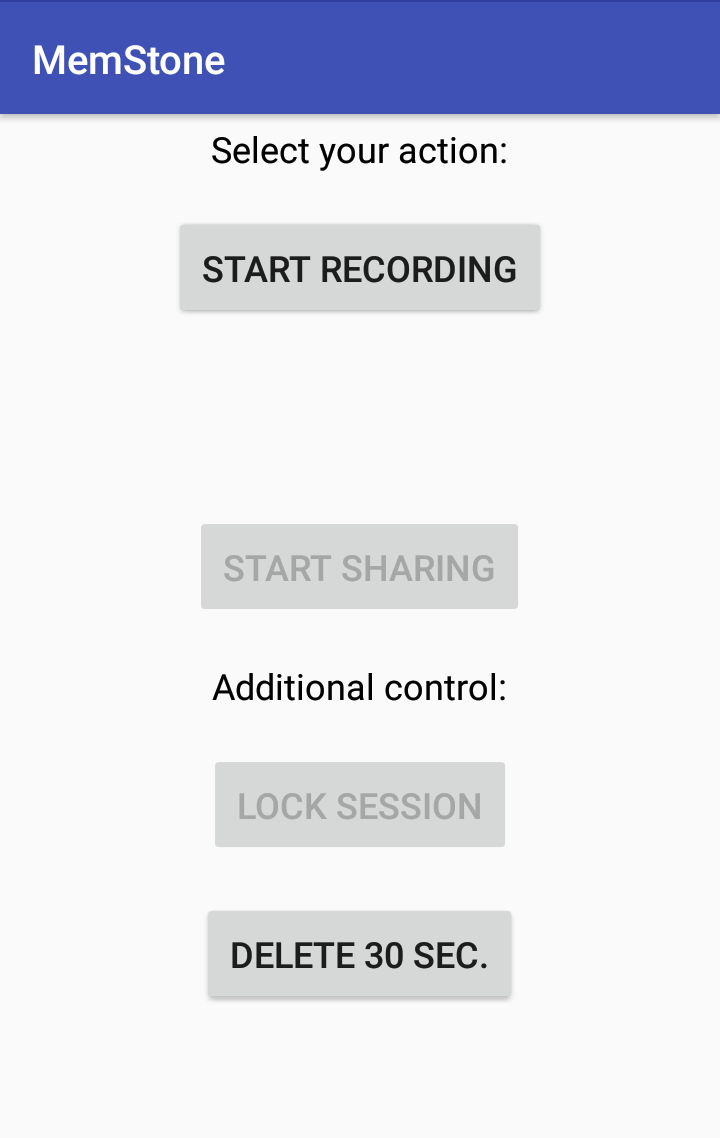
\includegraphics[width=0.31\textwidth]{Home_screen}
  \caption{Smartphone application user interface.}
  \label{figp1}
\end{figure}

The figure \ref{figp1} shows the home screen of the application. From figure \ref{figp1}, the application has four buttons which does the following actions: 
\begin{itemize}
\item Start Recording and Stop Recording
\item Start Sharing and Stop Sharing
\item Lock Session and Unlock Session
\item Delete last 30 seconds
\end{itemize}

The first three buttons are toggle push buttons which changes the state of the application when selected. For example, when the user selects start recording the button gets activated and label of the button changes to stop recording. When the application is not recording, the sharing and locking button will be disabled as shown in figure \ref{figp1}. When the application is not sharing the lock session button will be disabled since the application is recording for the user only and there is no need to lock the session. 

\begin{figure} [!ht]
\begin{subfigure}{0.31\textwidth}
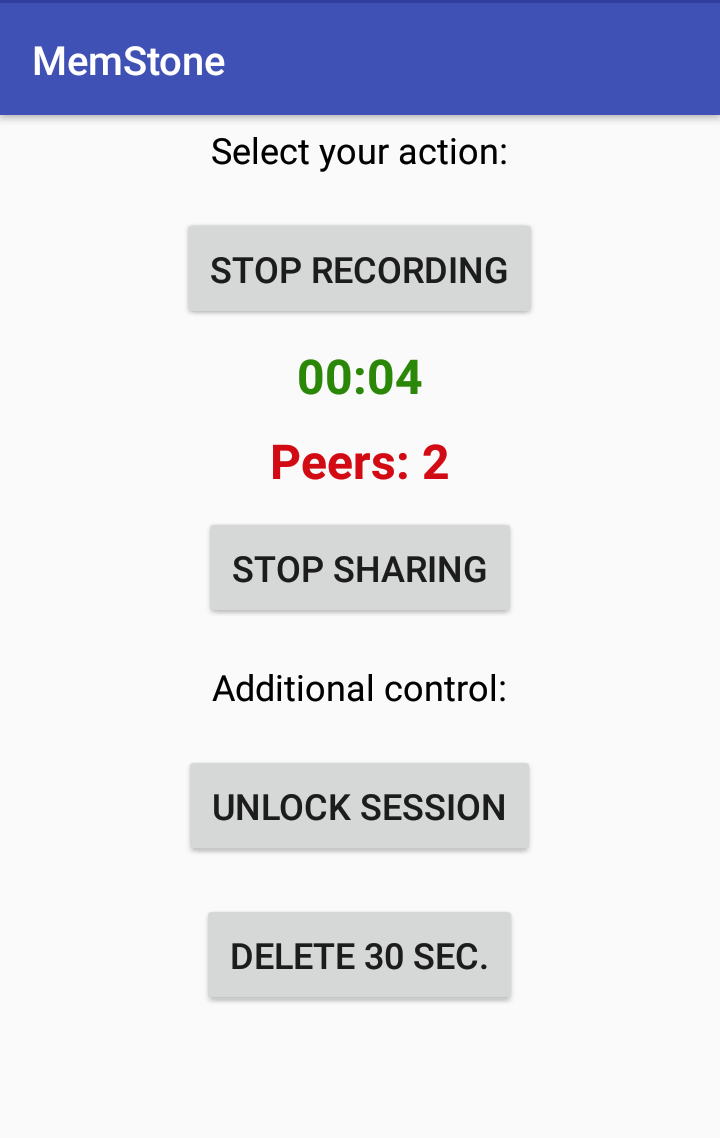
\includegraphics[width=\linewidth]{Lock_Session}
\caption{While sharing in a locked session.} \label{figp:1a}
\end{subfigure}
\hspace*{\fill} % separation between the subfigures
\begin{subfigure}{0.31\textwidth}
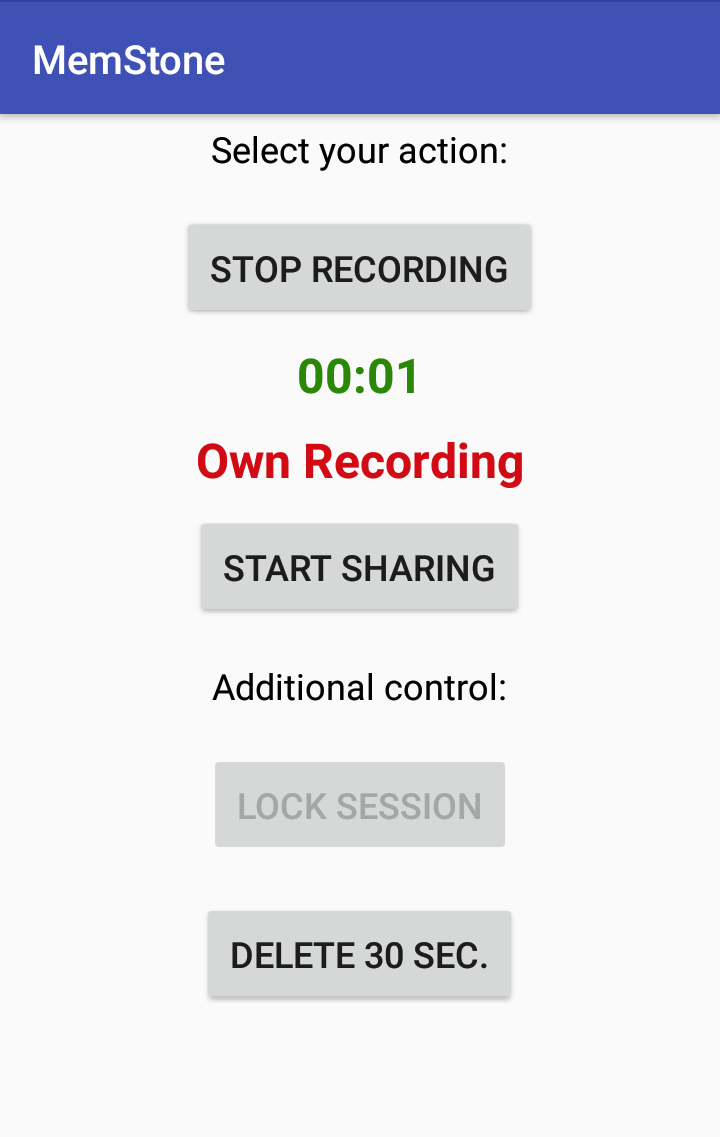
\includegraphics[width=\linewidth]{Recording}
\caption{While recording for oneself.} \label{figp:1b}
\end{subfigure}
\caption{Information displayed in smartphone application.} \label{figp:1}
\end{figure}

The application also notifies the user by showing the status message as "Own Recording" as shown in figure \ref{figp:1b}. And when the application is sharing it shows the the number of peers its currently sharing with as shown in figure \ref{figp:1a}. The application also displays the elapsed time since recording started as shown in figures \ref{figp:1}. When the user presses the "Delete 30 Sec." button it deletes the images that been captured for the past 30 seconds this also makes the timer to reset to less than 30 seconds and also the user can use this option multiple times. 

\chapter{Evaluation of the MemShare's prototype website}

This chapter will discuss how the evaluation experiments were designed, planned and conducted for evaluating the MemShare's prototype website. For this, the book "Handbook of usability testing: how to plan, design, and conduct effective tests" by \citeauthor{rubin_handbook_2008} was referred. This book gave a very good idea about how to design and conduct the experiments. This chapter also presents how the data is collected from the experiments and how it is analyzed. From the analyzed data, the usability problems that participants have faced during the evaluation are identified and results are presented in this chapter. Finally, the feedback and suggestions which were collected from participants are also presented in this chapter. 

\section{Experimental design}

The experiments were designed to evaluate the usability of the MemShare's prototype website. As mentioned before, the evaluation method chosen for evaluating the MemShare prototype website is usability testing where each participant was asked to complete a set of tasks using the prototype website. The type of usability testing method used is formative testing, this helps to gather data about participants efficiency, effectiveness and satisfaction on using the prototype website. Before conducting the experiments, a pilot session was conducted with one participant to fine-tune the experiment session. This helped to verify the chosen tasks for evaluation and whether the prototype is working properly or not for the chosen tasks. In the following sections, the objectives of this evaluation are explained, the research questions that this evaluation aimed to answer are presented, then how the data is collected from different data sources are explained and finally the tasks used for the experiments are presented.


\subsection{Objectives}
As mentioned in section \ref{obj}, the main objective of this evaluation is to assess the overall effectiveness on how the personal and shared lifelog data is presented and visualized in the prototype website. Furthermore, this evaluation also tries to identify the problems or obstacles for visualizing lifelog data.


\subsection{Research questions}
By keeping the objectives in mind, the research questions were formulated. These are the following research questions that this evaluation tries to answer:  
\begin{itemize}
\item Can participants easily and successfully identify the information presented in the website? 
\item Can participants successfully navigate and access the captured images taken during an event?
\item Can participants easily and successfully find and sort events based on location and date?
\item Are participants successful in annotating a memory cue and finding the annotated memory cue?
\item Do users like the way how captured information is organized into comprehensible units or "experience events"?
\item Do users like the overall visualization and transition animations present in the website? 
\end{itemize}

\subsection{Data collection}

To answer the afore mentioned research questions, performance data, preference data, suggestions and feedback were collected during the experiment session. The following topics briefly explain how the data is collected and what measures are taken.
\newline

\textbf{Experiment session:}

During the experiment session, performance measures such as task time (time taken to complete a given task by participants), errors (incorrect action taken by participants) and task success (whether participants could complete the given task) were collected while participants performs the given tasks. These measures are used to determine the effectiveness and efficiency of the MemShare prototype website. 
\newline

\textbf{Questionnaire:} 

At the beginning of the experiment session, participants were given a consent form to sign. The consent form did not include only demographic questions (such as age group and gender) but also asked participants to rate their internet browsing skills. This question was asked to understand whether participants are familiar with using a web user interface. The consent form can be found in appendix \ref{sec:consent}.

At the end of the experiment session, participants were asked to fill up a post questionnaire. This questionnaire is based on SUS (System Usability Scale) questionnaire developed by \citeauthor{brooke_sus-quick_1996}, which can be used to measure participants satisfaction after using the prototype website. The SUS questionnaire is chosen because it's a valuable evaluation tool to measure users subjective reactions for using the system and it has been proved to be reliable and robust \citep{brooke_sus:_2013}. According to \citeauthor{tullis_comparison_2004}, SUS is the best among the other free to use questionnaire and with a sample size of 8-12 participants a reliable result can be obtained. This questionnaire was mainly developed to evaluate systems but it can be modified to evaluate websites by changing the words of the questionnaire from "system" to "website" and "cumbersome" to "awkward" which doesn't affect the results \citep{bangor_determining_2009}. The format of the SUS questionnaire can be found out in appendix \ref{sec:sus}. This questionnaire has a set of ten statements which are either positive or negative and are ordered in alternating position. Each of these statements has a five-point scale which has a range from strongly disagree to strongly agree.
\newline

\textbf{Interview:} 

After the experiment session, a structured interview is conducted where participants were asked to answer a set of questions related to their experience on using the prototype website. These are the questions asked to each participant as listed in table \ref{tab0}. The interview session was also audio recorded. Feedback and suggestions were gathered from participants through the interview questions which would help to identify problems faced by participants while evaluating the prototype website and to further improve the website either functionally or visually.
\newline

\begin{table}[!ht]
\centering
\begin{tabular}{ll}
\hline
1 & What are your overall impressions of the website?                                                                                    \\ \hline
2 & Do you like the way how the information is organized in the website?                                                                 \\ \hline
3 & Do you like how contents or images are presented and visualized in the website?                                                      \\ \hline
4 & What are the features you like about the website?                                                                                    \\ \hline
5 & What are the features you least like about the website?                                                                              \\ \hline
6 & If you could make one significant change to this website, what change would you make?                                                \\ \hline
7 & \begin{tabular}[c]{@{}l@{}}Do you have any other questions or comments about the website or your experiences\\ with it?\end{tabular} \\ \hline
\end{tabular}
\caption{List of interview questions for evaluation of MemShare prototype website.}
\label{tab0}
\end{table}

\textbf{Observation and recordings:}

% How it helped for later viewing and cross checking the times and stuffs
The entire session was video recorded. During the experiment session, participants were asked to "think aloud" while they were interacting with the prototype website. This method allows participants to express their thoughts verbally while interacting with an interface. When participants come across a problem in the interface they identify the problem by saying it out aloud, these comments were noted down. Further, participants were asked to explain about the problem briefly in the interview session. The common misconception about this method is that it will influence the task completion timings but this was later proved not to be true by \citeauthor{hertzum_thinking_2013}. It is also being proved that participants perform faster while they "think aloud" because they think about a clearer approach to complete the task while they verbalize their thoughts \citep{doi:10.1080/01449299008924235}. Later these recording were played back and observed to further analyze the problem and what circumstances lead to the problem. The recording was also useful to cross check with the measures noted down during the experiment session such as task time.

\subsection{Tasks}

During the experiment, all participants were given a set of tasks to complete using the MemShare prototype website and they were asked to answer some questions about user interface. The tasks and questions are listed in table \ref{tab1}. There are 9 tasks and 2 warm up questions about the prototype website interface that were asked to participants. The warm up questions are meant to make participants familiarize with the prototype website user interface. Participants were asked to answer and complete the tasks in the order shown in table ~\ref{tab1}. Each of these tasks covers all the functionalities and visualization options present in the prototype website for participants to interact with. 

\begin{table}[!ht]
\centering
\resizebox{\textwidth}{!}{%
\begin{tabular}{ll}
\hline
Question 1 & From the homepage, how many events are there in the website?                                                                                                                 \\ \hline
Task 1     & Identify the co-located peers who were present for Event 1.                                                                                                                  \\ \hline
Question 2 & When did the other users arrive and left the activity in Event 1?                                                                                                            \\ \hline
Task 2     & \begin{tabular}[c]{@{}l@{}}In the home page, please try to find a picture that contains a document from\\ Nami’s timeline flow in Event 2.\end{tabular}                      \\ \hline
Task 3     & In the homepage, for Event 1 navigate and display all the images shared by Nenji.                                                                                            \\ \hline
Task 4     & Give the caption "Shadow" to the picture taken at 14:15pm by Nenji.                                                                                                          \\ \hline
Task 5     & Search for the image with the caption "Shadow".                                                                                                                              \\ \hline
Task 6     & \begin{tabular}[c]{@{}l@{}}In the homepage, display the fixed infrastructure camera as a participant in the\\ timeline and then access the images shared by it.\end{tabular} \\ \hline
Task 7     & In the homepage, access all the images both personal ones and shared ones captured during Event 1.                                                                           \\ \hline
Task 8     & \begin{tabular}[c]{@{}l@{}}In the homepage, sort and view the events that only took place at the location\\ USI Informatics.\end{tabular}                                    \\ \hline
Task 9     & \begin{tabular}[c]{@{}l@{}}Assuming there are many events displayed in the homepage, find an event that\\ happened on April 20, 2017.\end{tabular}                           \\ \hline
\end{tabular}%
}
\caption{List of questions and tasks given during the experiments.}
\label{tab1}
\end{table}

\section{Experiments}
All the experiments followed a set of predefined activities. At the beginning of the experiment session, participants were given a consent form to fill. The consent form and its contents can be found in appendix \ref{sec:consent}. The consent form was given to participants to get their permission to video record during the experiment session. The form also contains some demographic questions about participants. After participants fill out and sign the consent form, they were given a short introduction about the importance of the session, the rules of the session, the MemShare system and the prototype website. The session's introduction script can be found in appendix \ref{sec:sess}. After the introduction, participants were given a set of tasks to perform using the MemShare prototype website. While they were performing the task, the video was recorded and performance measures such as task time, errors and task success were noted down. The problems faced by participants and the comments given by participants while thinking aloud were also noted down in a data sheet, which can be found in appendix \ref{sec:data}. After completing all the given tasks, participants were given the SUS questionnaire to fill. At the end of the experiment, an interview was conducted to get feedback and suggestion from participants.


\begin{figure}[!ht]
  \centering
  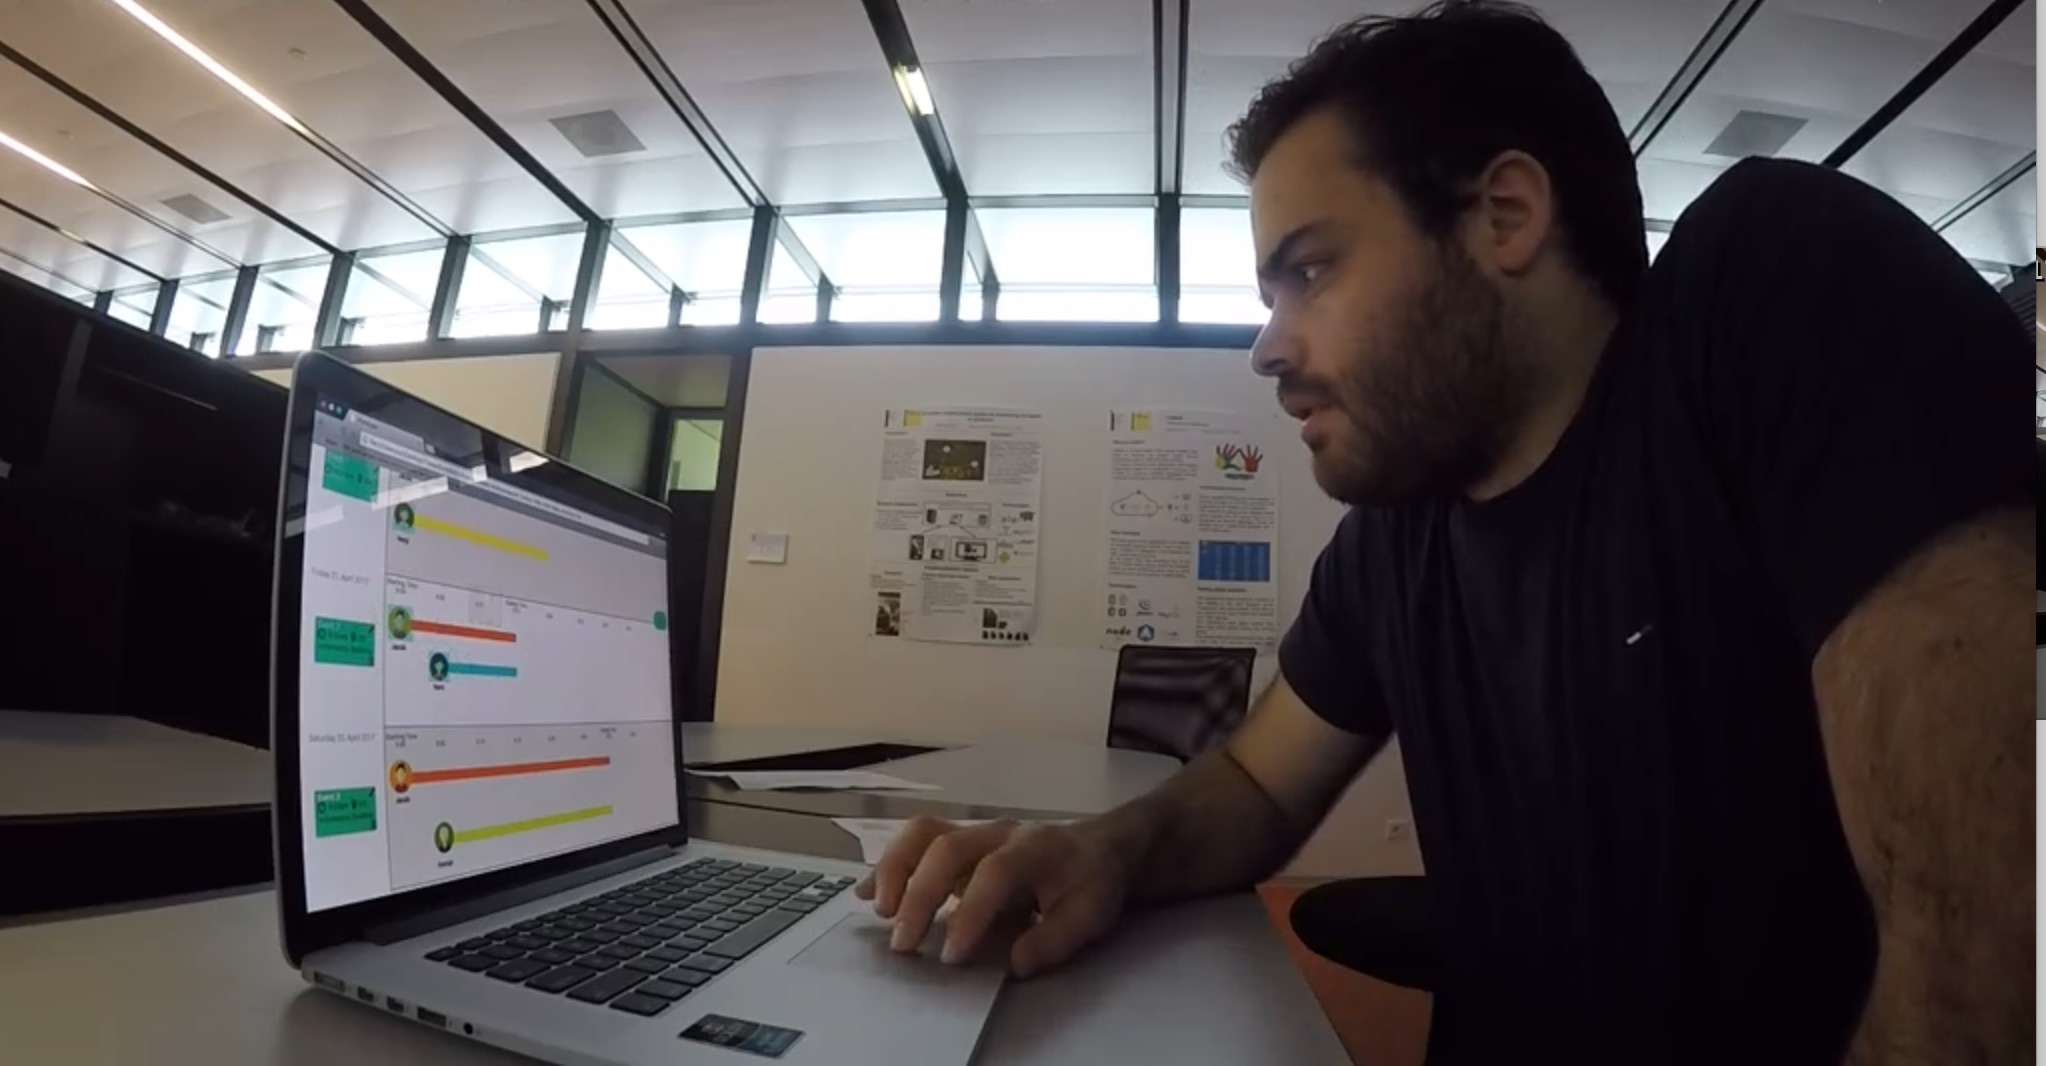
\includegraphics[width=0.7\textwidth]{Partic}
  \caption{Participant interacting with the prototype website during the experiment session.}
  \label{fig16}
\end{figure}
Eight participants were recruited for this evaluation. All participants were either Bachelor or Master students from Università della Svizzera Italiana (USI) in Lugano. \citeauthor{nielsen_jakob_why_2000}, reports that 80\% of usability problems can be found out by testing the product or interface with 5 participants. The experiments were conducted in a controlled setting and it took place at Università della Svizzera Italiana in Lugano. For the experiment session, participants were given a laptop with chrome browser to interact with the prototype website and the whole experiment session took around 30 minutes. 

\section{Results and discussion}
The following section describes about how the data from the experiments is analyzed and what are the results obtained from the analyzed data. In the subsequent sections, participants characteristic data is presented which was collected from the demographic questions on the consent form. Then results from the experiments and SUS score are presented and explained. Finally, participants suggestions and feedback are discussed in this section.

\subsection{Participants}

Out of the 8 participants from the experiments, 5 were male and 3 were female. The age group on which participants belong to is mentioned in table \ref{tab3} below.


\begin{table}[!ht]
\centering
\begin{tabular}{|l|l|}
\hline
Age Group & Number of participants \\ \hline
18-24     & 3                      \\ \hline
25-34     & 4                      \\ \hline
35-44     & 1                      \\ \hline
\end{tabular}
\caption{Number of participants and their age group.}
\label{tab3}
\end{table}

In the consent form after the demographic questions, participants were asked to rate about their internet browsing skill level. Out of the 8 participants, 5 of them identified themselves as expert, 2 of participants identified themselves as intermediate and 1 as novice.

\subsection{Experiments results} 
This section will present the results of the performance measures that are obtained from the experiments. From these results the effectiveness and efficiency of the prototype website can be understood.
\newline

\textbf{Task success:}

This metric is measured to find out whether participants could able to complete the given tasks using the prototype website. This measure is most commonly used to measure the effectiveness of an interface or product. When participants fail to complete a given task, it is noted down as 0 and when they succeed in completing the task it is noted as 1. This way of measuring task success is known as binary success \cite{albert2013measuring}. The successful completion rate for each task was calculated by taking the average of successful and non-successful tasks done by participants. Figure \ref{fig17} shows the result of successful completion rate for each task. 

\begin{figure}[!ht]
  \centering
  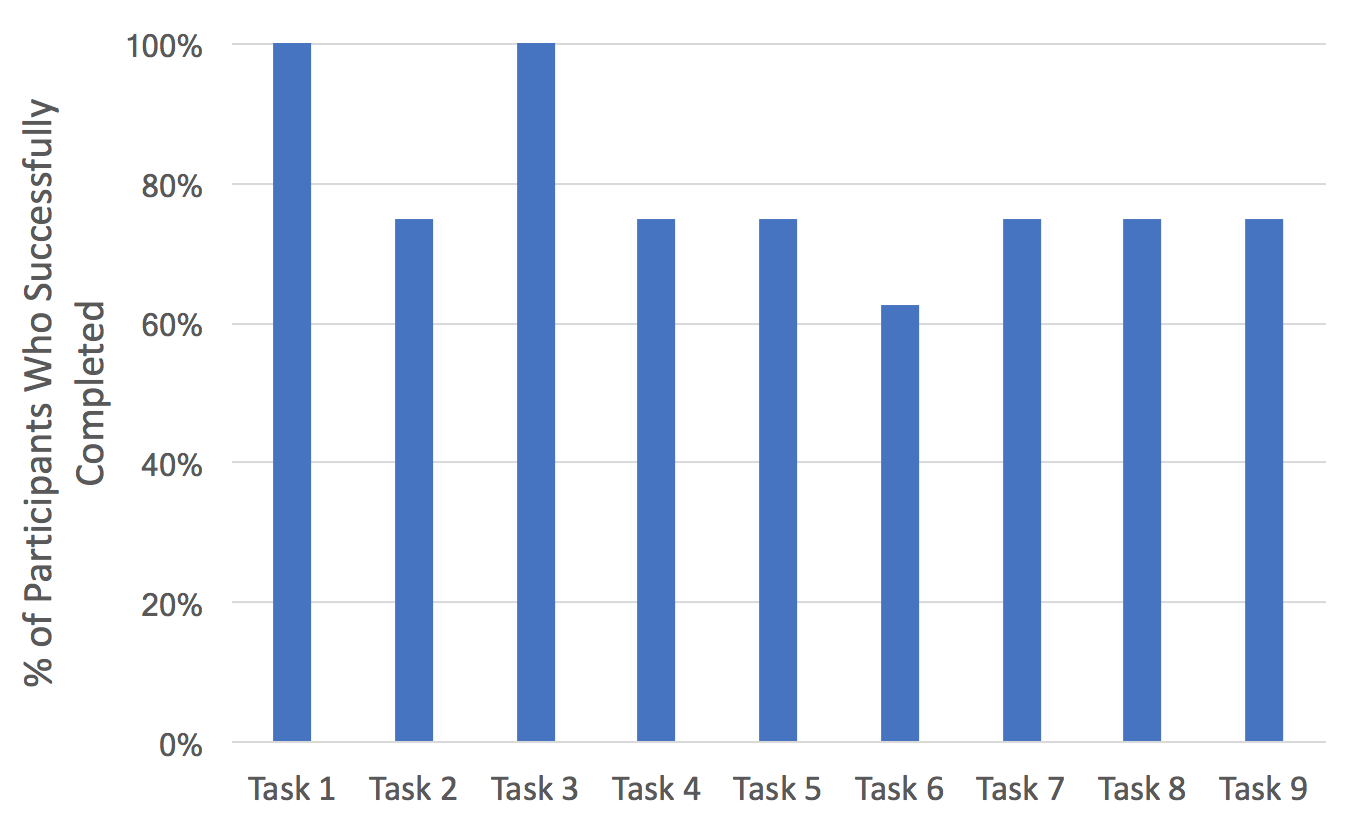
\includegraphics[width=0.8\textwidth]{wbTC}
  \caption{Task completion rate for each task.}
  \label{fig17}
\end{figure}

As shown in figure \ref{fig16}, tasks 1 and 3 were completed by all 8 participants. As listed in table \ref{tab4}, these two tasks involves in participants understanding the information presented in the homepage and accessing it. Task 2 has a completion rate of 75\% which means out of 8 participants, 2 failed in completing this task. This task is for participants to get to know about the visual transition present in the prototype website. The task 2 involves in participant to find an image from the timeflow bar. It is being observed that instead of using the timeflow bar to find the image, 2 participants directly accessed the peer's page to find the image. After completing the task 3, which is to access and the peer's captured images, participants were given task 4 to perform. For task 4, participants should give a caption to a captured image and only 75\% of participants were able to complete the task. Instead of giving the caption for the image, 2 participants described about the image. This shows that 2 participants didn't understand the task properly. For task 5 the completion rate is 75\%, for completing this task participants can either use the hidden search option in the co-located peer's page or using the hidden settings menu in homepage. It is being observed that 2 participants completely ignored the search option present in the peer's page. The lowest completion rate is for task 6, only 63\% of participants succeeded in completing this task. Therefore, out of 8 participants 3 of them failed in completing this task. Task 6 involves in displaying the infrastructure camera as a participant and for completing this task, participants should use the hidden settings and sorting options menu in the homepage of prototype. 2 participants couldn't find the hidden settings and sorting options menu and 1 participant couldn't able to find the option in the settings and sorting options menu. The Task 7 which is for visualizing all the images captured during the event has a completion rate of 75\%. For completing this task, participants have to click on the Event tag on the homepage and 2 participants failed to do the necessary action. Also for the task 8 and 9, the completion rate is 75\% therefore 8 out of 2 participants failed in completing this task. This task also involves in using the hidden settings and sorting options menu to sort and find the event based on location and date. 

\begin{table}[!ht]
\centering
\resizebox{\textwidth}{!}{%
\begin{tabular}{|l|l|}
\hline
Task order & Tasks                                                              \\ \hline
1          & Identify co-located peers.                                         \\ \hline
2          & Find an image from timeline flow bar.                               \\ \hline
3          & Display all pictures captured by co-located peer.                   \\ \hline
4          & Give caption to an image.                                           \\ \hline
5          & Search an image with its caption.                               \\ \hline
6          & Display the fixed infrastructure camera in timeline and access it. \\ \hline
7          & Access all images of an event.                                      \\ \hline
8          & Sort the events by location.                                         \\ \hline
9          & Find an event by date.                                              \\ \hline
\end{tabular}%
}
\caption{List of tasks performed by participants.}
\label{tab4}
\end{table}

\textbf{Errors:}

Errors made by participants for each task was noted down. Errors are nothing but incorrect actions which are made by participants while they were performing a task which sometimes can lead to a task failure itself. The incorrect actions can be taking an incorrect sequence of action, failing to take any action or making the wrong choice. Therefore, a task can have multiple errors and it is noted down after analyzing the recorded video taken during the experiment session. This measure is very useful for evaluating the navigability of the prototype website. This measure also can be used to measure the effectiveness of an interface or product. The total number of errors made by all participants for each task is added and figure \ref{fig18} shows the result obtained from it. As shown in figure \ref{fig18}, the task 6 and 7 has more frequency of errors compared to the rest of the tasks which has less than 4 errors. Only for task 1, there were 0 errors made by participants. This task involves in participants identifying the information present in the home page. The task 6 has frequency of 10 errors, this shows that participants have some difficulties in making the right action for completing this task. The task 6 involves in participants to enable the option for displaying the fixed infrastructure camera in the timeline and this option can be found in the hidden settings and sorting options menu. Also, the task 7 has an error frequency of 6 this shows that there is navigation problem to visualize all images captured in an event.


\begin{figure}[!ht]
  \centering
  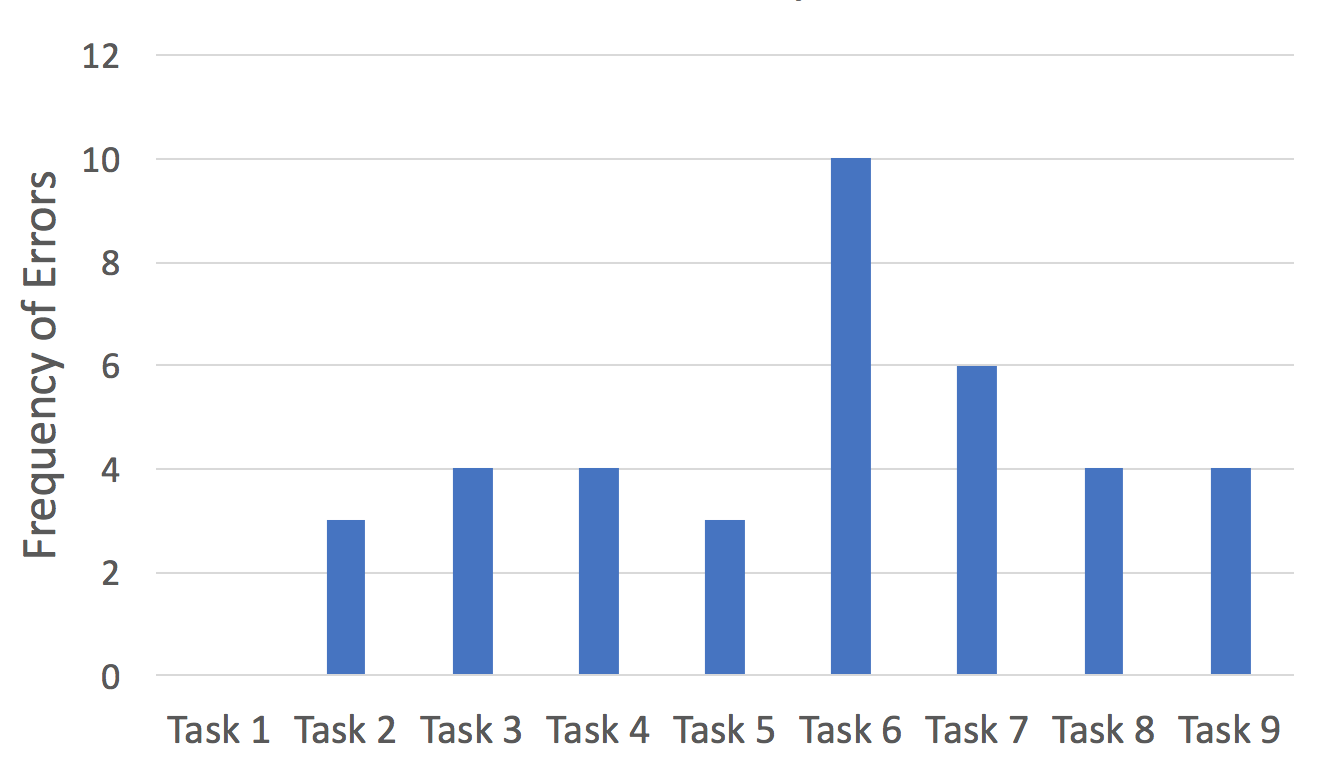
\includegraphics[width=0.9\textwidth]{wbE}
  \caption{Number of errors for each task.}
  \label{fig18}
\end{figure}

The Internet browsing skill level data gathered from the consent form helps to group participants according to their skill level. Out of 8 participants, 5 identified themselves as expert, 2 participants identified themselves as intermediate and 1 participant identified as novice. The average number of errors for all tasks made by each group is calculated and the result is shown in figure \ref{fig19}. From the image, it is noted that the novice participant made the highest number of errors which is 9 for all the tasks. The intermediate participants group made 7.5 errors on average for all the tasks. The experts group of participants made the least amount of errors which is 2.8 on average. This shows that expert participants didn't have much problems in using the prototype website to navigate and visualize the lifelog data. But both intermediate participants and novice participant had some difficulties in using the prototype website.  

\begin{figure}[!ht]
  \centering
  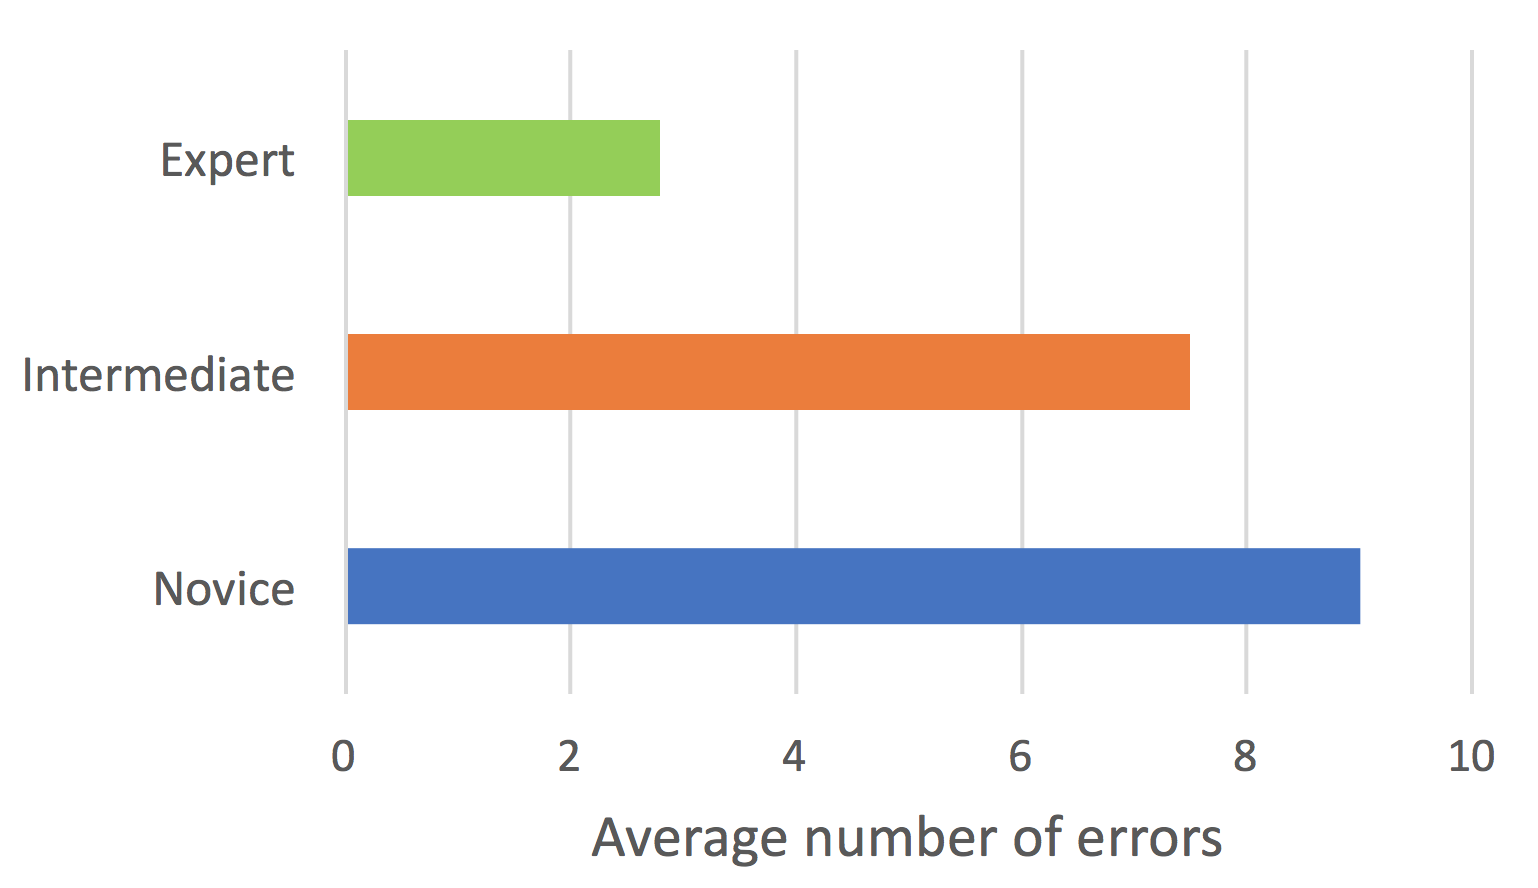
\includegraphics[width=0.7\textwidth]{Ebg}
  \caption{Average number of errors by participants group.}
  \label{fig19}
\end{figure}

\textbf{Efficiency:}

The most common way to measure efficiency is by measuring time on task. Since this evaluation is formative type of usability testing this metric will not be suitable for measuring efficiency. This metric would be more suitable for comparative type of usability testing where two versions of the product are evaluated by comparing each other. Another way to measure efficiency is to count the number of successful tasks completed by each participant and dived it by the total time spent for all task by that participant. This yields an efficiency score for each participants which corresponds to the number of tasks completed per minute by participant. This helps to understand how each participant performed the given tasks. Table \ref{tab6} shows each participant efficiency score and shows the number of task they have successfully completed and the total time spent for performing all the tasks. From table \ref{tab6}, the P1, P2 and P3 have the lowest efficiency score compared to the other participants. From the demographic data, it's been identified that participant P1 rated his Internet browsing skill level as novice and P2, P3 identified themselves as intermediate. The efficiency score of 0.66 means that participant P1 can finish 0.66 tasks per minute which is considerably low compared to participant P4 who can complete 7.01 tasks per minute using the prototype website. From calculating the efficiency score it has been understood that how the prototype website worked for each group of participants. It clearly shows users without any experience will find some difficulties while interacting with the prototype website. The type difficulties will be further explored in feedback and suggestions given by participants in next section \ref{fed}. 


\begin{table}[!ht]
\centering
\resizebox{\textwidth}{!}{%
\begin{tabular}{|l|l|l|l|}
\hline
Participants & Number of successfully completed tasks & Total time spent on tasks in minutes & Efficiency score \\ \hline
P1           & 2                          & 3.01                                 & 0.66             \\ \hline
P2           & 4                          & 2.44                                 & 1.46             \\ \hline
P3           & 9                          & 2.21                                 & 3.83             \\ \hline
P4           & 9                          & 1.17                                 & 7.01             \\ \hline
P5           & 8                          & 2.22                                 & 3.38             \\ \hline
P6           & 8                          & 2.48                                 & 2.86             \\ \hline
P7           & 8                          & 2.01                                 & 3.97             \\ \hline
P8           & 9                          & 2.18                                 & 3.42             \\ \hline
\end{tabular}%
}
\caption{Efficiency of each participant.}
\label{tab6}
\end{table}

\subsection{SUS score} % Satisfaction Measure 
The SUS questionnaire has ten statements with a five-scale range for each statement. To interpret the SUS score from the questionnaire there are three steps to follow:

\begin{itemize}
\item If the statement is odd numbered, subtract the given score by 1.
\item If the statement is even numbered, subtract 5 by the given score.
\item Add all the new values obtained from step 1 and step 2 and multiply the total by 2.5. 
\end{itemize}

\begin{figure}[!ht]
  \centering
  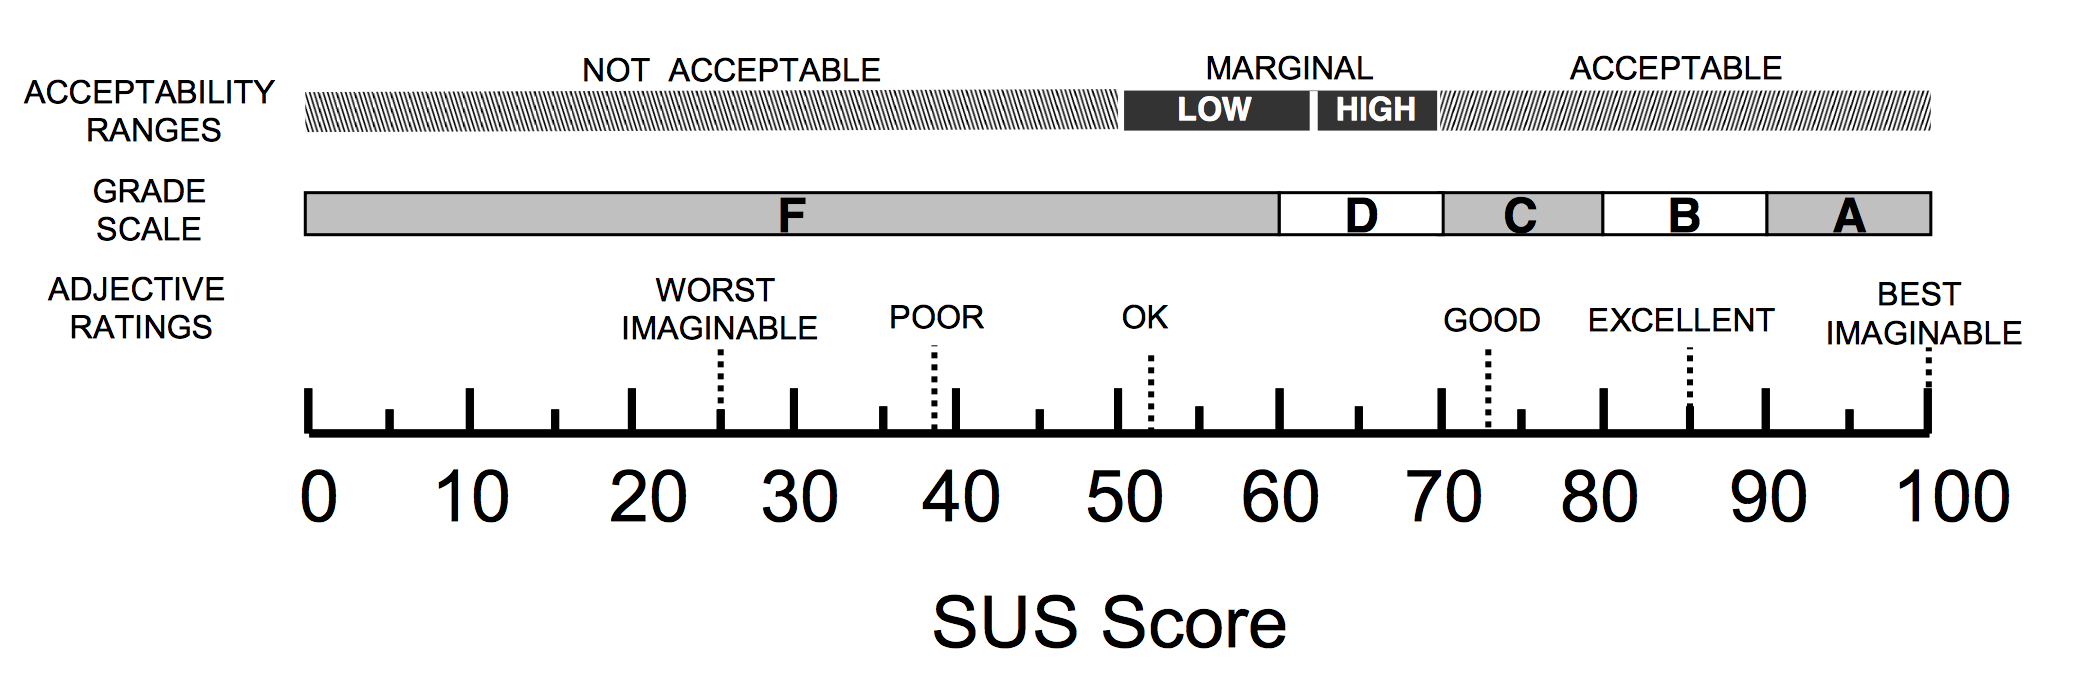
\includegraphics[width=0.9\textwidth]{susf}
  \caption{A comparison of the adjective ratings, acceptability scores, and school grading scales, in relation to the average SUS score \citep{bangor_determining_2009}.}
  \label{fig20}
\end{figure}

This yields a global usability score which ranges from 1-100 and this score can be interpreted from figure \ref{fig20} given by \citeauthor{bangor_determining_2009}, where they compare the SUS score with an adjective rating, school grading scale and acceptance range level. According to \citeauthor{bangor_determining_2009}, the adjective ratings highly correlates with the SUS score. Therefore, the SUS score can be interpreted from the adjective ratings scale. If the SUS score is above 73 then it is "Good" usability score. 

\begin{table}[!ht]
\centering
\begin{tabular}{|l|l|}
\hline
Participant Number & SUS Score \\ \hline
P1                 & 82.5      \\ \hline
P2                 & 90        \\ \hline
P3                 & 90        \\ \hline
P4                 & 72.9      \\ \hline
P5                 & 70        \\ \hline
P6                 & 72.5      \\ \hline
P7                 & 95        \\ \hline
P8                 & 75        \\ \hline
Average            & 80.9875   \\ \hline
Min                & 70        \\ \hline
Max                & 90        \\ \hline
\end{tabular}
\caption{SUS score given given by participants after evaluating MemShare prototype website.}
\label{tab7}
\end{table}

This table \ref{tab7} shows the SUS score given by each participant. The Minimum score given by participants is 70 which is a "Ok" score and the average is 80.98. From this result, it is known that participants were somewhat satisfied with the prototype website. 

\subsection{Feedback and suggestion}
\label{fed}
The recorded audio from the interview session is transcribed for each participant and the transcript for the whole interview session can be found on appendix \ref{mem:trans}. By analyzing the transcribed data, the usability problems were identified and valuable suggestions were also identified from this data. This data also helps us to understand what participants liked and disliked about the MemShare's prototype website. The following section will uncover the different aspects of the MemShare prototype website, which can be either positive or negative aspects and suggestions for making future improvements in the website.
\newline

\textbf{Information Organized in the site:}

Most participants liked how the information is presented and organized in the prototype website. Especially, they liked the timeline like interface which was easier to identify the information about the events. They also liked the how the images are presented in user's page which is also presented in a timeline like fashion.
\newline
\begin{adjustwidth}{1cm}{1cm}
\hspace{\parindent}P1: \textit{"I personally think you can just click the image and you can basically find everything from the timeline itself. How you display the contents of the timeline that is very clear."}

P6: "[..] \textit{I really like the feature that I can see the people who joined my day from an overview of the timeline, think this is a very good feature you should keep it }[..]."
\newline
\end{adjustwidth}
Participants also liked how the information is encapsulated into comprehensible units as events. So that it reduced the complexity of the information presented.
\newline
\begin{adjustwidth}{1cm}{1cm}
\hspace{\parindent}P3: \textit{"Yeah, its tidy and you can find almost all the information from a single page. I like this timeline with immediate feedback and also the filter is good and the way they are organized is good so there is a big event for each meeting for example and you can scroll all of them or sort them by date or something."}

P8: \textit{"But the information makes sense the way you encapsulated it completely makes sense. The timeline thing is really great absolutely that makes a lot of sense because you get ton of images from these things so the way its displayed perfect."}
\newline
\end{adjustwidth}
\textbf{Transition:}

Participants identified the transition effects present in the home page as a good feature. They liked the way, the timeline flow bar shows an overview of the captured images taken during the event while hovering on it. So that they won't even have to access the individuals pictures. They also like the feature which shows the four relevant pictures while hovering on the avatars of people which is presented in the timeline.
\newline
\begin{adjustwidth}{1cm}{1cm}
\hspace{\parindent}P3: \textit{"Yeah, they are clear and clearly shown without clicking you can have an immediate look for example of what happened at 14:15."}

P5: \textit{"[..] Yeah It is good when you go with the mouse over you can see like a preview and you can click}[..]."

P6: "[..] \textit{One feature I like is picture display when you moving hovering around the mouse you can see the pictures showing along the timeline I think this can do some links between the memory of the day and what happens so that's why it's a good feature.}[..]"

P7: "[..] \textit{Once you have the mouse on the icon you can see like some of the pictures so you don't need to really click on the user to check the pictures just you can stay on the home page and you still see the pictures so this is a plus.}"
\newline
\end{adjustwidth}

\textbf{Hidden settings and sorting options menu \& Search option:}

Most participants complained that the hidden settings and sorting option menu and search option present in the home page and individual's page. They explained that the option itself was overlooked by participants while performing the task. This is because the option wasn't obvious since it is displayed in the right side corner of the page. One participant mentioned that the icon of the hidden menu represents settings and it would be appropriate if it has a menu icon instead of the settings wheel to access the sorting options.
\newline
\begin{adjustwidth}{1cm}{1cm}
\hspace{\parindent}P1: "[..] \textit{I think the filter part you have to make it more obvious. Instead of the icon you can have more information about it [..] Just put the filter part try to display somewhere give a more obvious hint}"

P4: "\textit{I would change some of the icons that you have and I would change the settings bar into the menu bar}"
\newline
\end{adjustwidth}
Another suggestion given by participants is that the menu can be displayed somewhere else in the home page for example bellow the homepage menu.
\newline
\begin{adjustwidth}{1cm}{1cm}
\hspace{\parindent}P8: \textit{"[..] I don't like the options hidden here in settings on the right side I think those should go right under this Recall bar."}
\newline
\end{adjustwidth}
Also, participants didn't like the idea of the search option to be hidden and only by clicking it the search icon will make it accessible. Participants suggested instead of clicking it which would slide down another menu with the search bar, it would be better if the search bar shows up when the option is hovered by the mouse pointer. 
\newline
\begin{adjustwidth}{1cm}{1cm}
\hspace{\parindent}P5: "\textit{[..] What was not so clear was to do this search i mean they are hidden in this button here that look like preferences [..] Search for a caption maybe here could be some there is no information even if i go mouse hover and to make it a little more direct that would be more beneficial they a bit hidden the advance features.}"

P6: "\textit{[..] don't know what will happen if I click it only if I try it I will know it's maybe you can improve some on that part.}"
\newline
\end{adjustwidth}

\textbf{Infrastructure camera option:}

Few participants complained about enabling infrastructure camera option. They explained that the option is very small and it can be overlooked and only after spending some time in the interface they manage to complete the task. So, they suggest to make the option bigger or else the option can be implemented in the home page itself.
\newline
\hspace{\parindent}\begin{adjustwidth}{1cm}{1cm} 

\hspace{\parindent}P3: \textit{"The only difficulty I had is was to find the fixed camera maybe you should put there instead of putting it in the menu in the settings you should be put the bigger tick in the main page to show fixed camera photos."}

P7: \textit{"[..] The only thing is this view of the fixed infrastructure camera as a participant is not so clear and the box is too small so its not easy to see.}
\newline
\end{adjustwidth}

\textbf{Event Tag:}

Two participants gave their opinion about the event tag, the purpose of the event tag is not so clear for opening all the images of an event. One participant confused the timeflow bar to view all images of the event instead of using the event tag. Another participant suggests, instead of using a box shaped tag the event, it should be circler as that of peer's avatar in the timeline so that it would be easier to identify.
\newline
\begin{adjustwidth}{1cm}{1cm}
\hspace{\parindent}P5: "\textit{[..] If this to find all the images for one event wasn't so clear, I mean I realized that okay if i go with a mouse over here it changes to a link. I can click here but otherwise maybe that's not so clear i had to look for it that way.}"

P6: \textit{So for now I think is to re-organize the tag off the events to make it similar to a user's tag maybe not the same as a profile of a person but in the same shape a round shape with colored background.}
\newline
\end{adjustwidth}

\textbf{Problems with prototype: }

Most participants complained about the quality of the prototype, that it lacks clarity and the interface is not so smooth. Because of this reason the task related to "give caption to the image" was failed by some of participants and some took time to complete it. 
\newline
\begin{adjustwidth}{1cm}{1cm}
\hspace{\parindent}P4: "[..] \textit{Bit more clarity with the functionalities such as adding a caption i think the icon looks like i can edit the title instead.}"

P8: "\textit{[..] This glitching that happens is driving me nuts. [..] I don't like this the edit button which doesn't make any sense but this is this is very small"}
\newline
\newline
\end{adjustwidth}
\textbf{Suggestions:}

Some suggestions were given by participants to further improve the design of the website. For instance, one participant suggested highlighting the hovered options will solve some navigation problems and also if there is an option to scale down the thumbnail in individual's page it would be helpful to scroll through if there is a vast amount of images. Another participant suggested, an option to organize the event by alphabetic order would be easier to sort many events. Finally, one participant suggested to implement machine learning to the system itself to automatically give caption to the image.
\newline
\begin{adjustwidth}{1cm}{1cm}
\hspace{\parindent}P6: \textit{"There are some extra features you can add like what are the interactions with users shared with a day for example here I have a chess game with nenji you can automatically extract it"}

P7: \textit{"If you can give them a name then you can organize them by alphabetic order this can be a way to look for the event."}

P8: \textit{"Some Highlighting the options will be nice. [..] If you are able to give the dimension of the thumbnail it would be great, if i have 10000 images or something."}
\end{adjustwidth}
\section{Summary}  
The goal to evaluate the MemShare prototype website was achieved and the evaluation could answer the proposed research questions. From the experiment, participants could understand the information presented on the timeline like interface of the prototype website, for navigating and accessing the all images of an event some participants weren't able to complete the task. Some participants had some difficulties on using the hidden setting and sorting options menu and the search option present on the peer's page. 

From the feedback given by participants, it is observed that most participants preferred the timeline like interface and how the lifelog contents were arranged into events. Also, they liked the transition effects and animations present on the prototype website. 

The main usability problems identified from the evaluation is the hidden settings and sorting options menu which have the options to sort events, find images and the option to view infrastructure camera as a participant. The other usability problem identified from the evaluation is the event tag present in the home page. 

Some of the relevant suggestions made by participants will be taken into consideration for future improvement. This evaluation considers the MemShare prototype website as usable based on the SUS score given by participants. But further improvements must be made to improve the usability of the website. Thus, proving it is an effective web user interface to present and visualize lifelog data.   

Chapter \ref{chpcon} concludes this work and discusses on modifications and possible future implementations of the MemShare website.


\chapter{Evaluation of the MemStone tangible interface}

This chapter discusses about how the evaluation experiments were designed, planned and conducted for evaluating the MemStone tangible interface. In the subsequent sections of this chapter, the results from the analyzed quantitative data and qualitative data gathered from the experiments are presented. 

\section{Experimental design}
The experiments designed to evaluate the MemStone device, were similar to that of the experiments conducted for evaluating the MemShare prototype website. The usability testing method was used to evaluate the MemStone device. But instead of using formative type of usability testing, a comparison type of usability testing was done. In the experiments, the MemStone device was tested against with a smartphone user interface which has all the functions similar to that of the MemStone device. A description of both these interfaces can be found in section \ref{sec:mem}. The following sections explain the objective of this evaluation, the research questions that this evaluation tries to answer, the data collection process, and finally tasks used for experiments.

\subsection{Objective}
The main objective of this evaluation is to understand the strengths and weaknesses of the MemStone device. In addition, this evaluation tries to:
\begin{itemize}
\item Determine which interface was better in making data capturing and sharing decision. 
\item Gather feedback and opinions to further improve the MemStone device.
\end{itemize}

\subsection{Research questions}
By keeping the objectives in mind the research questions were formalized and this evaluation tries to answer them. These are the following research questions:
\begin{itemize}
 
\item Can participants successfully use the MemStone device to control the aspects of data sharing and data capturing compared to the smartphone application?

\item Can participants quickly interact with the MemStone device to control the aspects of data sharing and data capturing compared to the smartphone application? 

\item Do participants think the feedback given by the MemStone device is appropriate? 

\item Can participants successfully identify the information present on the MemStone device?

\item Which of the two interfaces would participants prefer for controlling capturing and sharing of their digital memories?

\end{itemize}

\subsection{Data collection}

This section will explain how the data was collected from the experiment session and the various data sources. The collected data helps to answer the afore mentioned research questions and to discover usability problems. These are the data sources:
\newline

\textbf{Experiment session:}

The experiment session has been divided into two parts, since it's a comparative test this involves in participants completing tasks with the MemStone device and with the smartphone application. Therefore, in each part of the experiment session, either the MemStone device or the smartphone application is evaluated by participants. While participants interact with the MemStone device and the smartphone application performance measures such as task time and task success were noted down. These measures will help us to understand the efficiency and effectiveness of MemStone device and how does it compare to the baseline smartphone application alternative.
\newline

\textbf{Questionnaires:}

Participants were given two questionnaires to fill, one of the questionnaires was a pre-questionnaire given at the start of the experiment session and a post-questionnaire was given after each time when participants finishes evaluating either the MemStone device or Smartphone application. The pre-questionnaire has questions related to demographics and regarding participants meeting information capturing preferences. These questions were asked to understand how participants capture information shared in meetings so far and to find out whether the MemStone device would be useful for capturing information during meetings. The format of the pre-questionnaire can be found in appendix \ref{ses:pre}. 

The post-questionnaire was based on SUS questionnaire \citep{brooke_sus-quick_1996} which has ten statements and these statements covered varies aspects of usability. At the end of the post questionnaire three additional statements were added with 5 points likert scale. These statements were added to measure participant's subjective assessment on intuitiveness, enjoyability and effectiveness of the MemStone device and the smartphone application which they have evaluated. The format of the post questionnaire can be found in the appendix \ref{ses:postq}. 
\newline

\textbf{Interview:}

At the end of the whole experiment session, participants were asked to answer some questions in a semi-structured interview session. The questions asked to participants were about their opinions on using images to capture information and their impressions on using the MemStone device and the smartphone application. Participants were also enquired whether they came across any difficulties while using the MemStone device and if they have any suggestions to improve the device in the future. The list of questions asked during the semi-structured interview session can be found on appendix \ref{ms:int}.
\newline

\textbf{Observation and Recordings:}

The whole session is video recorded while participants interact with the MemStone device and the smartphone application. Interview sessions were also audio recorded. The recorded video helps us to understand participants reactions while they were interacting with both the interfaces. The video recordings were also useful to calculate time spent by participants on each task and to cross check task success. The audio recordings were transcribed and analyzed to identify the problems faced by participants and to get suggestions which can further improve the MemStone device in the future.
 
\subsection{Tasks}
Instead of giving tasks to participants, a novel way was adopted to convey the tasks. This involves in using a scripted video, participants were asked to watch this and pretend to be one of the participant from the video, while they interact with MemStone device and smartphone application during the experiments session. The video shows a scripted meeting between a professor and his teaching assistant.

\begin{figure}[!ht]
  \centering
  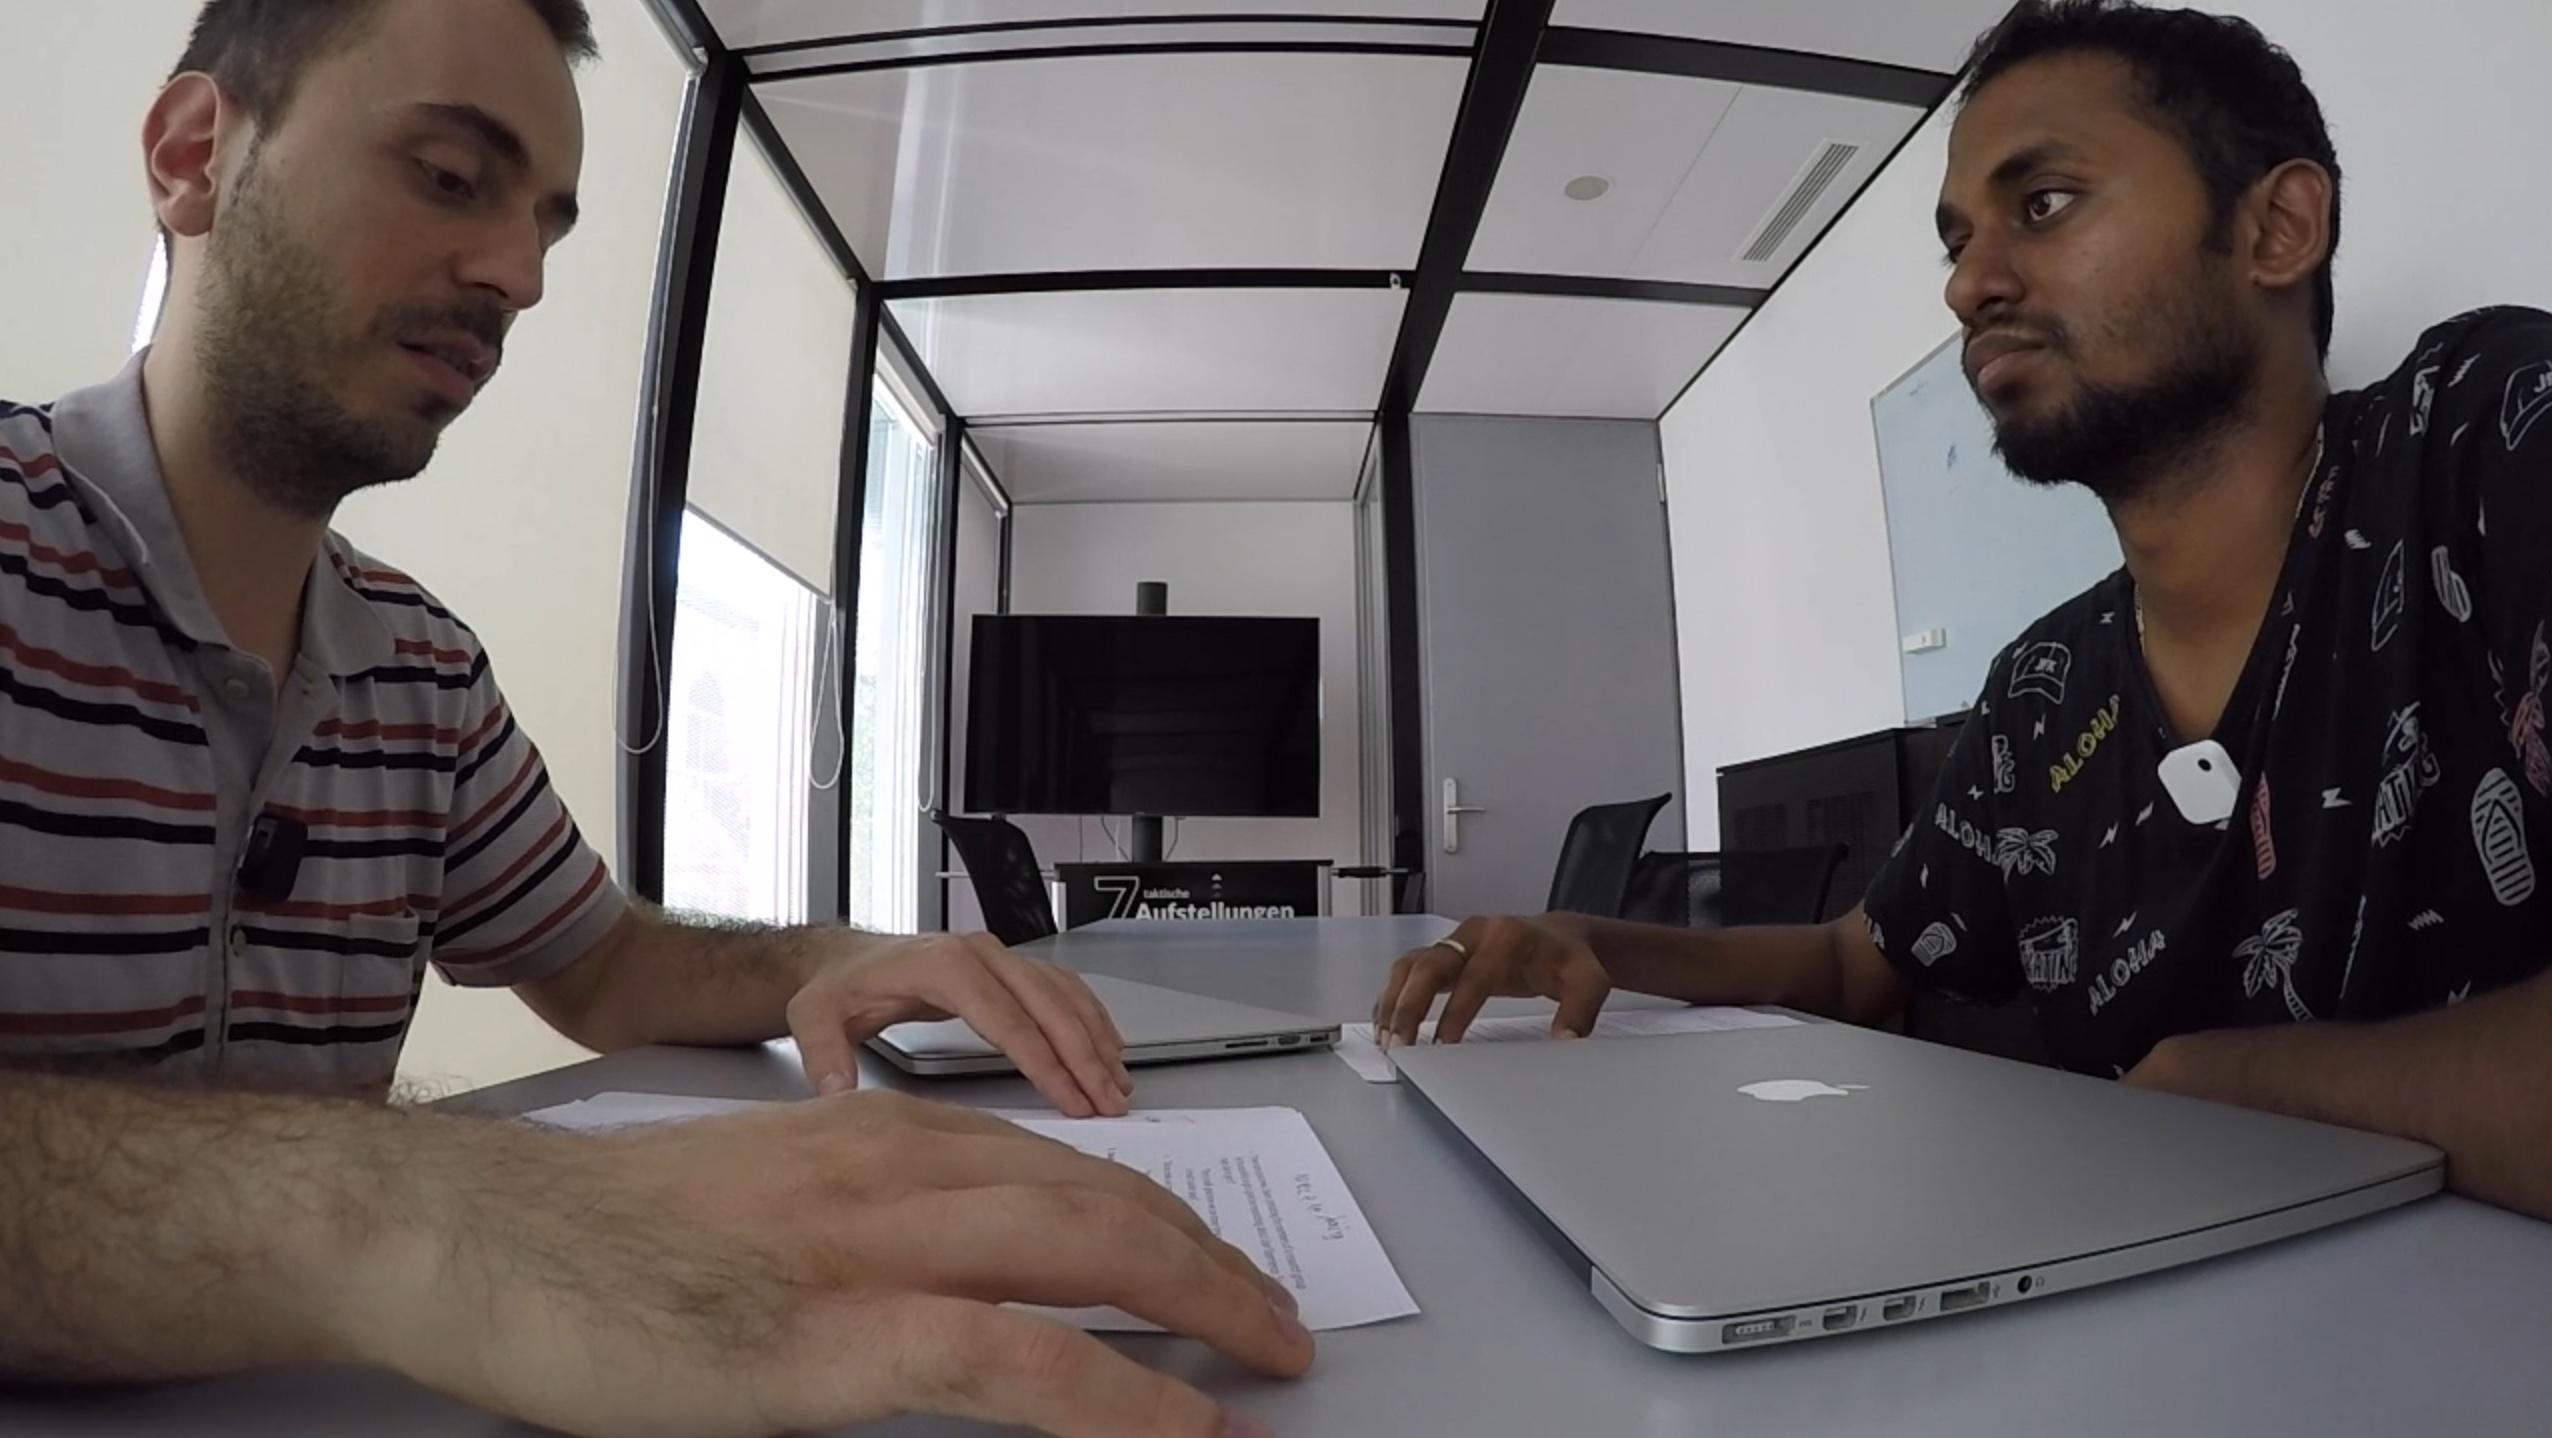
\includegraphics[width=0.7\textwidth]{videot}
  \caption{Screen-shot of the scripted video.}
  \label{fig21}
\end{figure}

In this video, there are audible clues present and by listening to the audible clues, participants have to preform the tasks. For example, in the scripted video if the professor informs to the teaching assistant "Let's record and share our meeting" after hearing this, participants must perform the suitable action with the MemStone device or the smartphone application. The scripted video has 10 audible clues for 10 tasks. Since the evaluation experiment involves in testing the MemStone device and smartphone application by participants, two scripted videos were made with different context and some of the tasks were shuffled. One scripted video is 15 minutes long and the another is 14 minutes long. Such two videos were created to avoid any learning bias, i.e., participants getting used to the video from the first part of the experiment, and then performing better while evaluating the other interface during the second part of the experiment. Table \ref{tab8} shows the tasks presented in each of the videos. Both videos have the same tasks and only the sequence of the task is slightly different. There are seven unique tasks and three of them are repeated. 

\begin{table}[!ht]
\centering
\begin{tabular}{|l|l|l|}
\hline
\textbf{Tasks} & \textbf{Script Video 1} & \textbf{Script Video 2} \\ \hline
1 & Record \& Share & Record \& Share \\ \hline
2 & Check time since sharing & Check time since sharing \\ \hline
3 & Stop Recording \& Sharing & Stop Recording \& Sharing \\ \hline
4 & Record Personally & Record Personally \\ \hline
5 & Record \& Share & Stop Recording \& Sharing \\ \hline
6 & Delete the last captured/shared image & Record \& Share \\ \hline
7 & Lock Session & Lock Session \\ \hline
8 & Verify Peers & Verify Peers \\ \hline
9 & Stop Recording \& Sharing & Delete the last captured/shared image \\ \hline
10 & Record Personally & Record Personally \\ \hline
\end{tabular}
\caption{Task sequence in both scripted videos.}
\label{tab8}
\end{table}
 

\section{Experiments}
Each of these experiments followed a set of activities. At the start of the experiment session, participants were given a consent form to sign. This consent form is to get the permission from participants to record video and audio during the test. The consent form can be found in appendix \ref{ses:con}. After participants fill up the consent form, the pre-questionnaire was given to them which has demographic question and questions related to participants preferences on how they capture information during meetings. Participants were given a short introduction about the session and the whole MemShare System was explained to them. In the introduction, the MemStone device and the smartphone application was introduced to participants but the functionalities of both the interfaces weren't mentioned to them. The introduction speech script can be found in appendix \ref{ses:intro}. About 12 participants were asked to evaluate the MemStone device and the smartphone application. 

The whole experiment session was divided into two parts, one for each interface (MemStone tangible interface and smartphone user interface). Since it was a comparative test, each participant were asked to evaluate the MemStone device and the smartphone application. To avoid biased results, the sequence of the interface presented to participants was shuffled and the script video were also shuffled between each participants. Table \ref{tab9} shows the sequence in which the interfaces are presented and which script video was used. This counterbalancing was important to avoid biased result and every possible combination of sequence was covered. 

\begin{table}[!ht]
\centering
\begin{tabular}{|l|l|l|}
\hline
\textbf{Participant} & \textbf{\begin{tabular}[c]{@{}l@{}}Interface presented and\\ Test video script used (Part 1)\end{tabular}} & \textbf{\begin{tabular}[c]{@{}l@{}}Interface presented and\\ Test video script used (Part 2)\end{tabular}} \\ \hline
P1 & MemStone Device - Script 1 & Phone App - Script 2 \\ \hline
P2 & Phone App - Script 1 & MemStone Device - Script 2 \\ \hline
P3 & MemStone Device - Script 2 & Phone App - Script 1 \\ \hline
P4 & Phone App - Script 2 & MemStone Device - Script 1 \\ \hline
P5 & MemStone Device - Script 1 & Phone App - Script 2 \\ \hline
P6 & Phone App - Script 1 & MemStone Device - Script 2 \\ \hline
P7 & MemStone Device - Script 2 & Phone App - Script 1 \\ \hline
P8 & Phone App - Script 2 & MemStone Device - Script 1 \\ \hline
P9 & MemStone Device - Script 1 & Phone App - Script 2 \\ \hline
P10 & Phone App - Script 1 & MemStone Device - Script 2 \\ \hline
P11 & MemStone Device - Script 2 & Phone App - Script 1 \\ \hline
P12 & Phone App - Script 2 & MemStone Device - Script 1 \\ \hline
\end{tabular}
\caption{Sequence in which the interface is evaluated by participants and script video sequence for each participants.}
\label{tab9}
\end{table}

A training session for using the interface was provided to participants according to their sequence. In this training session, all the functionalities of the respective interface was explained and participants were given some time to get familiarize with the interface. To explain the training session a document was given to participants, this document covers all the functionalities of the interface so that participants can read the document and understand it. The training session document for both the interfaces can be found on appendix \ref{ses:tra}. After the training session, participants were informed about the scripted video and they were requested to use the MemStone device or smartphone application according to the audible clues present in the videos. Participants were requested to act according to the clues given by the professor to the teaching assistant in the video. The task success measure and participants reactions were noted down while they were watching the video and interacting with the interface. After they watch the complete video, a post-questionnaire was given to participants to fill which is based on the SUS questionnaire and this questionnaire has three more statements related to intuitiveness, enjoyability and effectiveness of the interface which they have evaluated. In the next part of the experiment session, the other interface was presented to participants and it was evaluated with the same set of activities followed in the first part of the experiment session. Finally, a semi-structured interview session was conducted with participants where some questions were asked to gather feedback and suggestions. 

\begin{figure}[!ht]
  \centering
  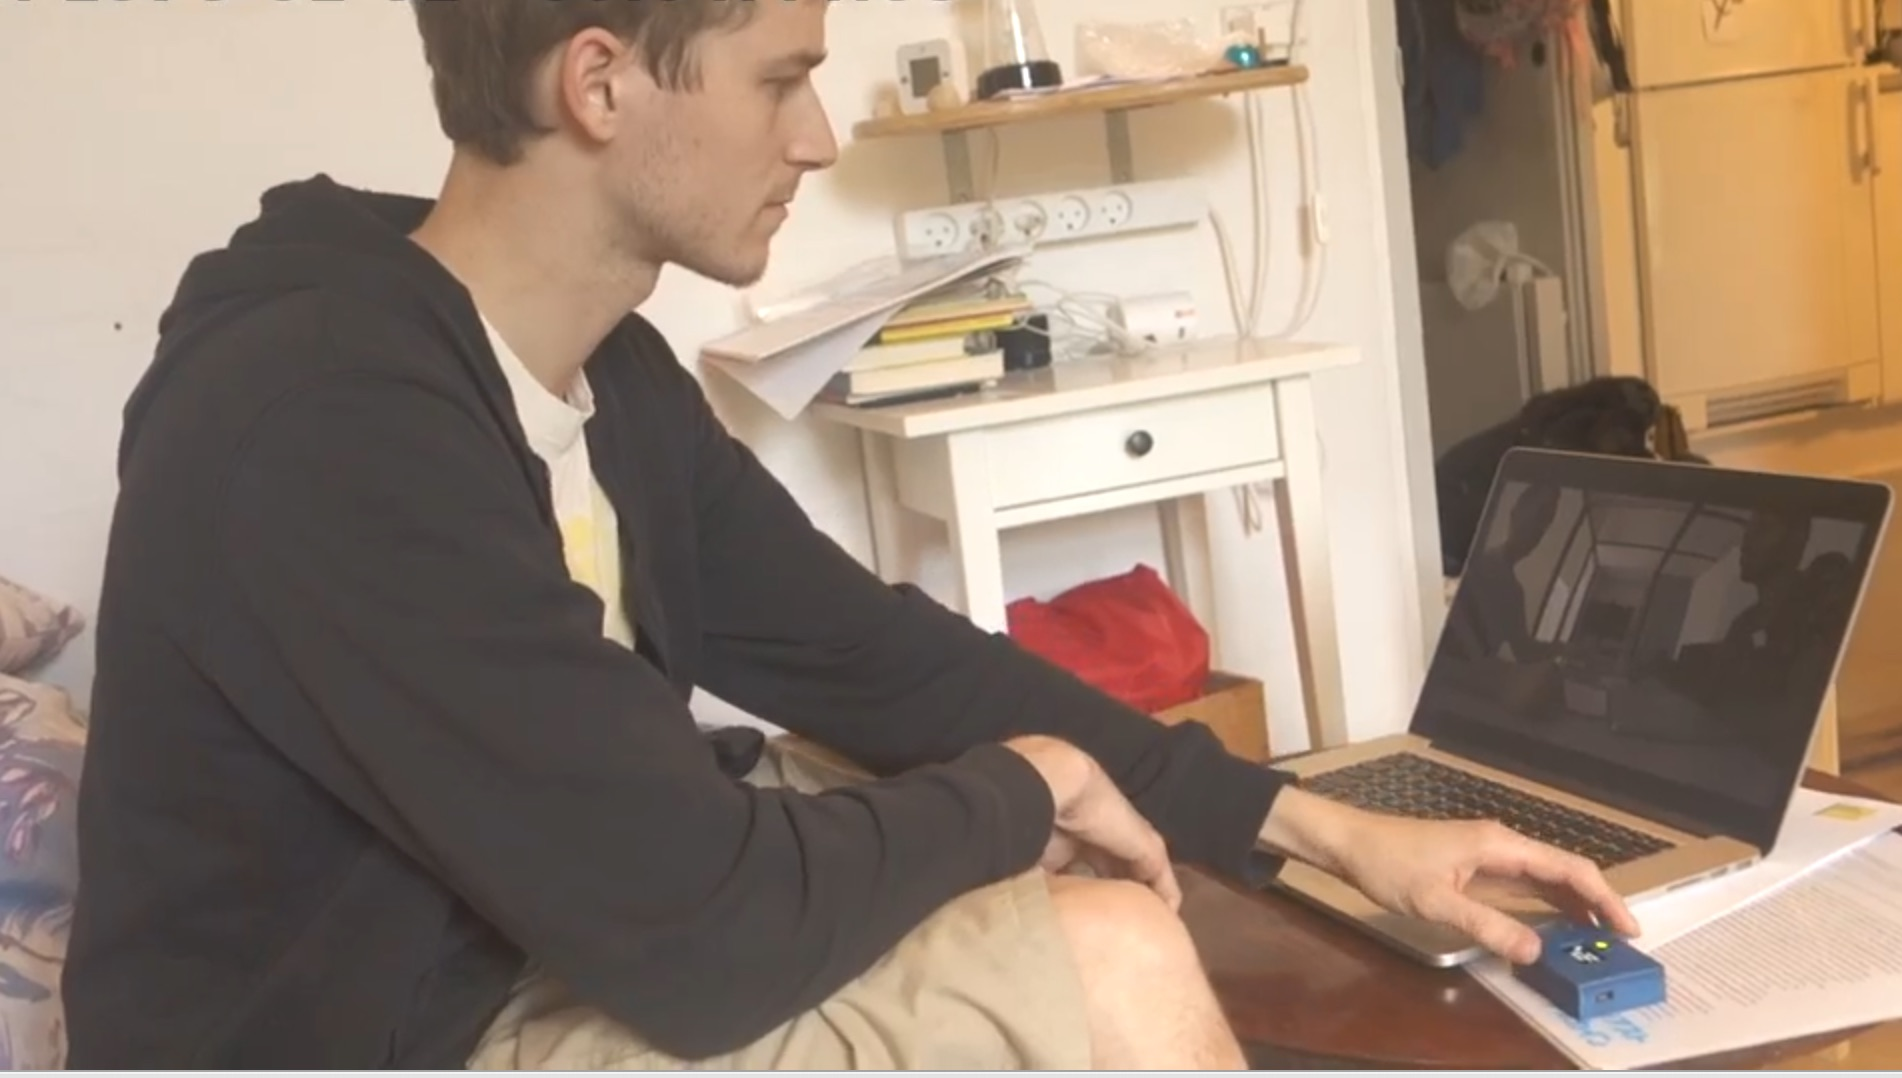
\includegraphics[width=0.7\textwidth]{Partic2}
  \caption{Participant interacting with the MemStone device as he watches the scripted video during experiment session.}
  \label{figp}
\end{figure}

The whole experiment session is conducted in a control setting inside a closed room with no disturbance from outside. They were given a laptop to view the video and the experiment session was video recorded with a camera. The audio was captured during the interview session with an android phone. 

\section{Results and discussion}
This section is about how the data from the experiments is analyzed and the results from the analyzed data are presented. From the results, the usability problems can be identified. In the subsequent sections, participants characteristics, the quantitative and qualitative results obtained from the experiments are discussed briefly.  

\subsection{Participants}
In total, 12 participants were asked to evaluate the MemStone device and the smartphone application. The demographic data is collected through the pre-questionnaire from participants to have a better understanding of their characteristics. Out of 12 participants 8 (67\%) were male and 4 (33\%) of participants were female. About 5 (42\%) participants where in the age between 18-24, 6 (50\%) participants were in the age between 25-34 and 1 (8\%) was above 60 years. Most participants have a master degree 50\% (6 participants), 42\% (5 participants) had a Bachelor degree or currently pursuing Masters and 8\% (1 participant) had a high-school diploma who is currently studying bachelors. Out of 12, 10 (83\%) participants used android phones and 2 (17\%) participants used iPhones. 

\subsection{Quantitative results}
This section will explain the process of how the performance measures were analyzed and what is the result obtained from it. Main reason for this analysis is to find out which interface is better between the MemStone device and smartphone application. From the beginning of the evaluation, 2 participants were not so engaged and it felt like they were forced to do the evaluation. As a result, their data was discarded from further analysis. 
\newline

\textbf{Task success:}

Since, the two video scripts have different task sequences for analyzing the data they were arranged in an order as shown in table \ref{tab20}. 

\begin{table}[!ht]
\centering
\begin{tabular}{|l|l|}
\hline
Task number & Task Description            \\ \hline
Task 1      & Record \& Share             \\ \hline
Task 2      & Check time since sharing    \\ \hline
Task 3      & Stop Recording \& Sharing   \\ \hline
Task 4      & Record Personally           \\ \hline
Task 5      & Record \& Share 2           \\ \hline
Task 6      & Delete                      \\ \hline
Task 7      & Lock                        \\ \hline
Task 8      & Verify Peers                \\ \hline
Task 9      & Stop Recording \& Sharing 2 \\ \hline
Task 10     & Record Personally 2         \\ \hline
\end{tabular}
\caption{Task order and description.}
\label{tab20}
\end{table}

The task success for each task was noted down during the experiment session, if participants succeeded in completing the task, it was noted down as 1 and if they failed to complete the task it was noted down as 0. By taking the average of the task successes and failures of each task, the successful task completion rate was calculated. The successful task completion rate for MemStone device and smartphone application was calculated. Figure \ref{fig22} shows the successful task completion rate by task. 

\begin{figure}[!ht] 
  \centering
  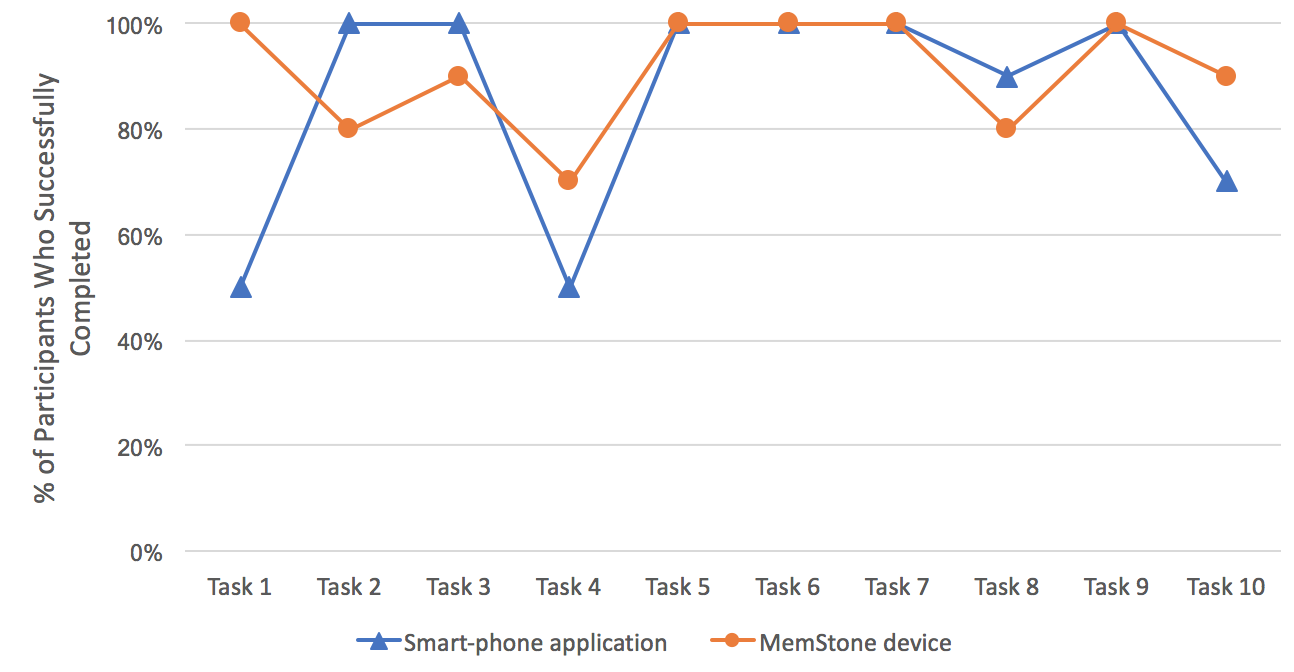
\includegraphics[width=0.9\textwidth]{tcm}
  \caption{Successful completion rate by task for MemStone device \& smartphone application.}
  \label{fig22}
\end{figure}

From figure \ref{fig22}, the task 1 completion rate for the smartphone application is 50\%. The task 1 corresponds to the task to record \& share, this is because participants should do two actions to complete this task in the smartphone application and most of them only performed one action as a result it was noted down as a failure. While performing for the second time all participants were successful in the task 5 for smartphone application. For both task 1 \& 5 in the MemStone device result there is no failure. The task 4 also has a completion rate of 50\% in smartphone application and for MemStone its 70\% this is because some participants were confused for performing this task. During the experiment session, participants were only told to do the actions done by the teaching assistant in the scripted video and this task 4 was performed by the professor and later the teaching assistant also performed it, so some participants thought they didn't have to perform it. Therefore, the MemStone device and smartphone application have a low completion rate. The task 4 to record personally is repeated in task 10, it can be observed that some participants also made the same mistake again. The task 2 for MemStone device has a completion rate of 80\%, this task involves participants to check the screen and 2 participants didn't check the MemStone screen. Also, similarly 2 participants didn't check the MemStone screen for task 8 resulting in 80\% of successful completion rate. Comparing with the task result of the smartphone application, participants performed better in completing both the task 3 and 8. The successful completion rate for task 3 for the MemStone device is 90\% therefore 1 participant didn't successfully complete this task. By checking the recorded video, it is observed that the participant had some language issue and he got confused to complete the task. Overall, participants while using the smartphone application performed badly for some of the tasks whereas using the MemStone device they performed slightly better. 
\newline

\textbf{Task time:}

The time spent by participants for completing each task is noted down in seconds. According to \citeauthor{albert2013measuring}, ideally the task time for even unsuccessful tasks should also be noted down but participants must know when to give up on the unsuccessful task. In our case, since the video is shown to participants and it is continuous therefore, when participants miss a task they might not know about it. They also suggest that, if the moderator should decide to end an unsuccessful task it is better to note down only the times for successful tasks. Therefore, for this evaluation only the times of successful tasks were noted down. Also, for calculating the average time for each task geometric mean is used which is less biased and it is more appropriate for calculating the mean for time data since such data is typically skewed \citep{albert2013measuring}. 

\begin{figure}[!ht]
  \centering
  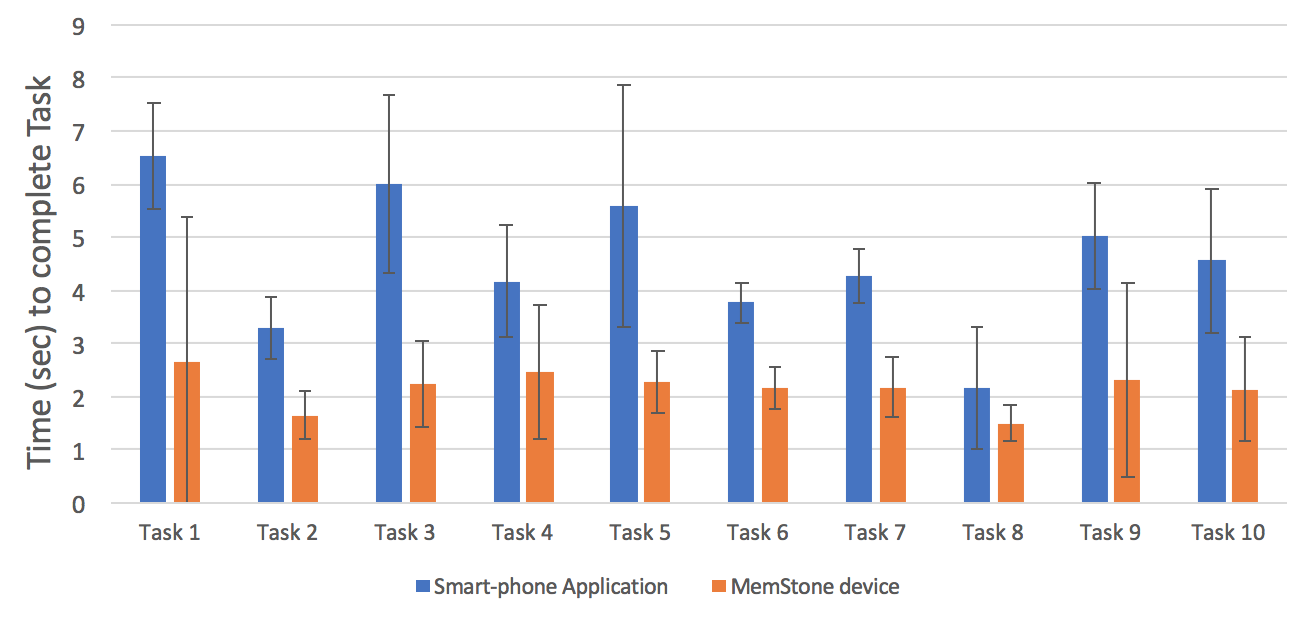
\includegraphics[width=1\textwidth]{ttm}
  \caption{Geometric mean time for all tasks by the MemStone device and the smartphone application.}
  \label{fig23}
\end{figure}

The graph figure \ref{fig23} shows the geometric mean time for all tasks performed by participants using the MemStone device and the smartphone application. The graph also shows the 95\% confidence intervals for each geometric mean time with error bars and this shows the variability in the data. From figure \ref{fig23}, it is observed that participants took more time to complete the tasks using the smartphone application than using the MemStone device. Therefore, it clearly shows that MemStone is more efficient. Even with the maximum confidence value for tasks, participants would be efficient using the MemStone device.
\newline
\newline

\textbf{SUS score:}

The SUS questionnaire given at the end of each part of the experiments session was analyzed and the SUS score for the smartphone application and the MemStone device was calculated. Table \ref{tab10} shows the SUS score given by each participants for the smartphone application and the MemStone device. Table \ref{tab10} also shows the average SUS score of the smartphone application and the MemStone device. The smartphone application has a SUS score of 86.25, based on the adjective scale given by \citeauthor{bangor_determining_2009} the score is interpreted as excellent and for the average SUS score for the MemStone device is 77.5 which can be interpreted as good. 
\begin{table}[!ht]
\centering
\begin{tabular}{|l|l|l|}
\hline
\textbf{Participants} & \textbf{Smartphone application SUS score} & \textbf{MemStone device SUS score} \\ \hline
P1                    & 65                                 & 77.5                        \\ \hline
P2                    & 87.5                               & 92.5                        \\ \hline
P3                    & 95                                 & 70                          \\ \hline
P4                    & 87.5                               & 62.5                        \\ \hline
P5                    & 72.5                               & 82.5                        \\ \hline
P6                    & 85                                 & 82.5                        \\ \hline
P7                    & 100                                & 90                          \\ \hline
P8                    & 85                                 & 80                          \\ \hline
P9                    & 97.5                               & 90                          \\ \hline
P10                   & 87.5                               & 47.5                        \\ \hline
\textbf{Average}      & 86.25                              & 77.5                        \\ \hline
\textbf{STD}          & 10.75290658                        & 14.04358296                 \\ \hline
\textbf{Min}          & 65                                 & 47.5                        \\ \hline
\textbf{Max}          & 100                                & 92.5                        \\ \hline
\end{tabular}
\caption{SUS score given given by participants after evaluating the MemStone device and the smartphone application.}
\label{tab10}
\end{table}

To measure participants subjective assessment on intuitiveness, enjoyability and effectiveness on the MemStone device and smartphone application few statements were provided at the end of the post-questionnaire with a Likert scale.

Participants average score for efficiency, intuitiveness, and enjoyability measures were calculated for the MemStone device and the smartphone application. Figure \ref{fig24} shows the results obtained from calculating the average score of the three aspects. From figure \ref{fig24}, the average score of the MemStone device intuitiveness is more compared to the smartphone application score and the average score of enjoyability that the MemStone device is more compared to the smartphone application score. Only in the aspect of efficiency the MemStone device score is low compared to the smartphone application. This might be because of the MemStone device is still a prototype. 
\begin{figure}[!ht]
  \centering
  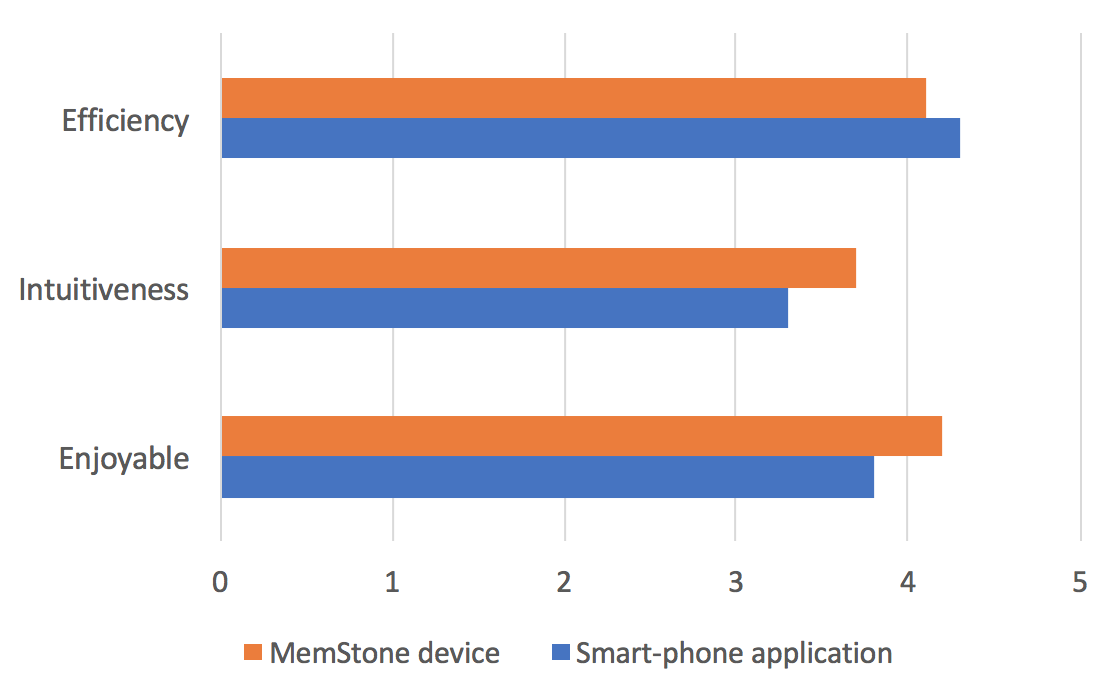
\includegraphics[width=0.8\textwidth]{qa}
  \caption{Average responses to three aspects for the MemStone device \& the smartphone application}
  \label{fig24}
\end{figure}


\subsection{Qualitative results}
The qualitative data was collected from the pre-questionnaire and also from the interview session. This section will discuss about the results obtained from both sources. 
\subsection*{Pre-questionnaire}
There were some open questions and closed question present in the pre-questionnaire which ask about participants preferences for capturing information during a meeting. This data was collected in order to understand how they have been capturing information so far and if they have any problem with it. To analyze the data obtained from the closed questions the frequency of each response is calculated. Only the responses for some of the intriguing questions will be presented in this section.
\newline

For the question - “Do you share the captured notes of your meeting?”

8 (75\%) participants responded they capture information whereas the rest of the 2 (25\%) participants responded they don't capture any information shared during the meeting.
\newline

For the question – “How do you capture your meetings” 

Participants capture meeting information by using paper notes approx. 50\% (7 Participants) and 3 (30\%) participants responded they use electronic notes application such as Google docs.
\newline

For the question – “What kind of information do you share during or after your meetings with others”

4 participants responded that it is mainly notes, 3 participants responded "Minutes of the meeting" and only one participant answered tasks to do list. 
\newline

For analyzing open questions, content analysis technique was used and it involves in categorizing the data where the frequency of occurrence is studied. The frequency act as an indicator for importance on the theme or concept. 

One of the category identified is on the topic about the disadvantages of taking notes in which participants explain the different reasons. 
\newline

\textbf{Taking notes disadvantages:}

The different reasons mentioned by participants are difficulty to concentrate and taking notes will miss the context. 
\newline
\hspace{\parindent}\begin{adjustwidth}{1cm}{1cm}
\hspace{\parindent}P2: \textit{"Problems faced difficult to concentrate while writing notes."}

P5: \textit{"To stay awake and force myself to listen [..]"}

P7: \textit{"Points could be discussed really quick and sometimes I have lost track of it and missed couple of points."}

P2: \textit{"People mimics cannot be captured and its important part of communication as a consequence the underlying meaning can be lost or misunderstood"}

P4: \textit{"Sometimes context is missing."}
\newline
\end{adjustwidth}

The obtained results gives an insight about participants capturing preferences. They mainly use notes to capture information and the notes don't provide all the information such as the context of the meeting and it is hard to focus on the meeting while taking notes.

\subsection*{Interview session}
The qualitative data collected from the interview session is transcribed and the transcribed script can be found in appendix \ref{mem:mt}. To analyze and interpret the qualitative data the whole transcript was read to understand about the data and any impression about the data was noted down. Then, the transcript was read again to identify themes and patterns in the data. These can be ideas, incidents, preferences and concepts. These identified themes and patterns were coded, which is to assigning labels to the text. For coding the text, the emergent coding approach was used. In this approach, the themes emerge from the text itself and the relevant theme is used to code the text instead of using predefined themes to code the text \citep{lazar2017research}. The codes with similar characteristics are identified to form a meaningful category and subcategories. From these categories, patterns where identified and connections were found. The connections are made within the categories are mostly about the problems identified by participants about the MemStone device and solutions given by participants to rectify the problem.

These are the categories which are identified from the analysis and they are presented below:
\newline

\subsubsection*{Image-based memory augmentation}
Some participants were expressing about their opinions about the idea of using images to augment memory. Therefore, a number of sub-categories were identified and these are the following sub-categories: 
\newline

1. \textbf{Benefits of using images to augment memory}

Most participants expressed about the different benefits of using images to augment memory where they explained that the images provide better context of an event and it can be useful in some situations like a presentation or a while standing in front of a white-board. They also explained that it is useful to keep track of daily activities and one participant explained that images capture mimics and hand gestures of the meeting participants and it is very useful to understand the situation. 
\newline
\hspace{\parindent}\begin{adjustwidth}{1cm}{1cm}

\hspace{\parindent}P1: \textit{"It won't give all the details but it will just provide some context that you can glance back at."}

P2: \textit{"[..] you will capture the mimics of the other person that is 80\% of all the communication that goes on through mimics and how you move your hands(gestures) so I think it's good."}

P10: \textit{"[..] if I'm sitting on the first row and you are sitting in the back and you cannot see it clearly and I can see it from the first row and share the pictures of the slides [..]".}

P7: \textit{"I think that's good it keeps the track off all the things we do [..]".}
\newline
\end{adjustwidth}

2. \textbf{Comparing images with other forms for capturing information}

Some participants even compared images to other forms of capturing information and identified that it is better compared to other forms such as text and video. 
\newline
\hspace{\parindent}\begin{adjustwidth}{1cm}{1cm}

\hspace{\parindent}P2: \textit{"I think it can be very useful especially in comparison in taking written notes [..]."}

P5: \textit{"It easily gets confusing, too much video is a bad thing. Still images are okay because you get information overlook."}

P7: \textit{"[..] if I write from a notepad or word I kind of lose track  of what's happening."}

P8: \textit{"It's relatively easy compared to taking down [..]."}
\newline
\end{adjustwidth}

3. \textbf{Drawbacks of capturing information through images}

Participants also identified that the images will not capture all the details of an event, sometimes it also captures random information according to the user position. Some participants raised their concerns about capturing information through images, that they won't be so confident to completely rely on images only. 
\newline
\hspace{\parindent}\begin{adjustwidth}{1cm}{1cm}
\hspace{\parindent}P1: \textit{"It won't give all the details [..]."} 

P1: \textit{"Although it might sort of random what is captured according to your position, it won't capture that unless you stand right front of it [..]."}

P3: \textit{"I am not very convinced about sharing images would make effective communication for a meeting."}

P6: \textit{"I can see the effect of the video of having like recordings with the video but with images I would still forget a lot of stuff."}

P9: \textit{"I personally couldn't imagine myself making the best use of the image honestly."}
\newline
\end{adjustwidth}

4. \textbf{Suggestions for capturing information}

To address the drawbacks of capturing images, participants suggested the MemStone system should also capture sound and one participant also suggested to automatically extract text from the event. 
\newline
\hspace{\parindent}\begin{adjustwidth}{1cm}{1cm}
\hspace{\parindent}P2: \textit{"I also think that recording sound can also be very useful especially if you're sitting in a meeting the important people if you are disagreeing, you have to come to some agreement, it would be really handy to have it as well."}

P9:\textit{ "I think if it has some the words they said are available I think it would be great it's simply because meeting is exchanged of information and opinion and so on."}
\newline
\end{adjustwidth}

\subsubsection*{Making Sharing decision }
This category talks about participants concerns while using MemStone device on meetings and how it will affect others present during the meeting.
\newline

1. \textbf{MemStone device influences sharing decision}

Some participants mentioned that using the MemStone device will influences other users in their sharing decision and its obvious than smartphone application.
\newline
\hspace{\parindent}\begin{adjustwidth}{1cm}{1cm}
\hspace{\parindent}P1: \textit{"Yeah, I guess that could influence their sharing decisions of others [..] But with the app that's not visible."}

P4: \textit{"I guess it's more obvious than if you use the phone app."}

P7: \textit{"They might be curious to see what I'm doing for some instance if they can easily know whether I'm sharing or not so they might be a little offended."}
\newline
\end{adjustwidth}

2. \textbf{Causes for sharing decision influence}

They also explain some of the reasons which will impact on making sharing decisions, one participant explains because of the social influence of other users. It is also noted from one of participant, if there is a higher official present during the meeting they will not be able to make sharing decision freely with the MemStone device. One of the participants explains that for making the sharing decision this will cause awkwardness and affect feelings of other users. 
\newline
\hspace{\parindent}\begin{adjustwidth}{1cm}{1cm}
\hspace{\parindent}P2:\textit{ " Yes, I think because people are very sensitive to other mean and what other people do and we usually follow. I think if one erases then everyone will start to erasing as well."}

P7: \textit{"[..] if I'm the boss it's fine but if I'm still the lower side employer or something then the boss wouldn't feel good about it so I think that could cause a problem."}

P9: \textit{"[..]it might be little bit awkward for example if you do double tap and you locked out and then if other people know [..]"}
\newline
\end{adjustwidth}


\subsubsection*{Gestures reliability and limitations}

This category talks about the problems experienced by participants on using the MemStone device gestures and their concerns on the reliability of the gestures. They also gave some suggestion to implement in the device.
\newline

1. \textbf{Problems with gesture}

Some participants were not so sure about how the locking feature worked and many participants didn't like the tapping gesture for locking since it would disturb other peers. One of the participant also mentions that while using the shake gesture to delete it is hard to look at the screen and that you might even delete more images or delete none.
\newline
\hspace{\parindent}\begin{adjustwidth}{1cm}{1cm}
\hspace{\parindent}P1:\textit{"Tapping on the device could shake it and then that's a bit ambiguous."}

P4: \textit{"[..]shaking you don't really know, I mean you kind of see whether it works but when you shake it's hard to see whether its erased or no."}
\newline
\end{adjustwidth}

2. \textbf{Concerns about gestures reliability }

Most participants preferred to use the smartphone application because it's assuring than MemStone device. Maybe this is because of the device still in its prototype phase and some gestures didn't work properly and since the smartphone application has a bigger screen to view the status. 
\newline
\hspace{\parindent}\begin{adjustwidth}{1cm}{1cm}
\hspace{\parindent}P4: \textit{"I think the gestures should work completely perfect every time otherwise you can accidentally record something that you are not supposed."}

P4: \textit{"I probably prefer to use the phone app just because you are more confident that it works."}
\newline
\end{adjustwidth}

3. \textbf{Gesture improvements}

To rectify the above mentioned problems, participants suggested changing the gesture for locking or implementing a separate physical button in the device for lock and delete.
\newline
\hspace{\parindent}\begin{adjustwidth}{1cm}{1cm}
\hspace{\parindent}P5: \textit{"Idea of locking should use another expression. Because locking and unlocking is sort of broader than what you actually intended to do."}

P7: \textit{"[..]to delete and lock it I think probably some easier gesture could be used probably to make it simpler probably a button because that is quicker."}
\newline
\end{adjustwidth}

\subsubsection*{The MemStone concept}
These subcategories are related to the identified good and bad aspects of the MemStone device. Also, the suggestions and the future prospects of the device is explained in this category.
\newline

1. \textbf{Good characteristics of device}

Participants response about the characteristics of the device were diverse. Most of the responses were positive that the device is fun to use, physically visible compared to the smartphone application, resembles like a toy, user friendly and one of the participant mentioned that MemStone device would provide a better work-flow during meetings.   
\newline
\hspace{\parindent}\begin{adjustwidth}{1cm}{1cm}
\hspace{\parindent}P1: \textit{"The physical device, it's nice to that turn it around. If you sit by a table, it's like it's a nice device to interact with.}"

P1: \textit{"So the device it provides much better workflow when you use the MemStone as a tool in your meetings."}

P2: \textit{"It was really fun to use."}

P3: \textit{"It's a simple nice tool."}

P4: \textit{"Well it does seem like a prototype but I like how it is visible compared to the app you can easily see whether it's recording or not."}

P7: \textit{"It was easy to use [..]"}

P6: \textit{"Well I like the device. I like the design of it and I mean it's kind of like a toy the device I liked. "}

P9: \textit{"I think it looks pretty cool and it was very easy to use."}
\newline
\end{adjustwidth}

2. \textbf{Inconveniences with the device}

Most participants mentioned that they wouldn't like to carry around the MemStone device and they mentioned that they have to get used to the device gestures which will be an inconvenience.
\newline
\hspace{\parindent}\begin{adjustwidth}{1cm}{1cm}
\hspace{\parindent}P3: \textit{"I don't like to carry too many electronic devices around and just trying to have one electronic device makes it better than having too many tools."}

P4: \textit{"I think it's one more thing to carry around in your pocket which is kind of annoying."}

P6:\textit{ "[..] it takes more effort in a way you to remember to bring it and I guess you need to charge it as well."}

P7: \textit{"[..]phone is something that we have with us all the time so and the app is really easy to use."}

P9: \textit{"I don't like having two stuffs at the same time so it was good but I couldn't see it's there just for that function."}

P10:\textit{ "The disadvantage of this you have to memorize for example if you shake it the information will be deleted or you turn it this side or that side it takes time to memorize."}
\newline
\end{adjustwidth}

3. \textbf{Suggestion for physical improvements}

One of the participants mentioned instead of carrying two devices the camera and the MemStone device separately it can be integrated with the camera itself which would solve the problem of carrying too many devices. Also, some participants also gave other suggestions such as using a bigger touch screen to display information, an extra LED for locking and also some aesthetic improvements.
\newline
\hspace{\parindent}\begin{adjustwidth}{1cm}{1cm}
\hspace{\parindent}P1: \textit{"[..] need a bigger display to show that information."}

P2: \textit{"[..] bit lighter so that it fixes in a shirt pocket."}

P4: \textit{"I think it should have extra LED for locking."}

P4: \textit{"I think integrating with the camera itself would make a lot of sense maybe the camera itself could have some similarities to show whether it's recording or not and whether it's sharing and so on."}

P7: \textit{"[..] instead of double tap probably I would do something like a touch sensor or some kind of movement other kind of moment."}

P10: \textit{"[..]make it more colorful I don't know it's just like a pager to make it more interesting."}
\newline
\end{adjustwidth}

4. \textbf{Future prospects of device}

Two of the participants mentioned that if the MemStone gets integrated in meetings itself and if everybody uses the MemStone device it won't cause any disturbance or it won't cause discomfort in making sharing decisions.  
\newline
\hspace{\parindent}\begin{adjustwidth}{1cm}{1cm}
\hspace{\parindent}P6:\textit{"I think probably at the beginning people will noticing it but after a few meetings you know it will get integrated into. So, I don't think anyone would notice it anymore."}

P8:\textit{"Not really but it might be a little disturbance to other people so if everyone in the room or everyone in the meeting is using it I don't think it's an issue."}
\newline
\end{adjustwidth}


\subsubsection*{Privacy and security}
These sub-categories explain about participants response on security and privacy issues on using the MemStone device. Participants also gave some suggestions to rectify the issues. 

1. \textbf{Concerns about privacy \& security}

Most participants were concerned about the peer's details, for example with whom the information is shared and they were concerned about proximity radius for sharing. Participants also mention, while using the device the user should be careful on doing the gestures and doing the wrong gesture would results in sharing of sensitive information. 
\newline
\hspace{\parindent}\begin{adjustwidth}{1cm}{1cm}
\hspace{\parindent}P1:\textit{"I guess if there is sensitive data what is shared and you don't lock the peers someone could come close by and the tap-off of the information." }

P2: \textit{"I didn't see the other peer who was also interacting in the meeting."}

P2:\textit{"[..] it's about human error. Of course, you should be a little bit careful or thoughtful of it."}

P3:\textit{ "I think just saying the number of peers under the device kind of doesn't tell you really who you are sharing with."}

P3:\textit{"It's more Public whether you're sharing data are not but you don't really have full confidence whether it's working whether its recognizing the gestures."}

P8: \textit{"[..]even a small change in gesture and without noticing its change you might share sensitive information."}

P10: \textit{"Yes, but you should be careful with your gestures [..] by accident you can share some confidential information."}
\newline
\end{adjustwidth}

2. \textbf{Suggestions for functional improvements}

For addressing the above mentioned issues of security and privacy, participants gave some suggestions to improve the functional aspects of the MemStone device. One of the suggestion is to have option to create a user profile itself on the device and to show more information about peers. Participants also gave other suggestions such as having a active preview of the data which has been captured, a starter guide in the device and a calendar with reminder option. 
\newline
\hspace{\parindent}\begin{adjustwidth}{1cm}{1cm}
\hspace{\parindent}P1: \textit{"[..] more functionality like seeing what peers are connected specifically or something like that with more information, that could be on the device perhaps that could be useful."}

P1: \textit{"[..] maybe to create a user profile or something on the device so that you type in our name and your device has a name."}

P3: \textit{"The display of the captured information would be nice."}

P4: \textit{"I can't have an active preview of the data of its recording I would prefer that it could be a part of it."}

P5: \textit{"But I think a lot of information can be put on the MemStone itself so it becomes self-explanatory because people don't want to read manuals."}

P10: \textit{"Maybe like a calendar to see which date is today like time and date [..]add some reminder for example during the meeting like group reminder is something additional."}
\newline
\end{adjustwidth}

\subsubsection*{Device interaction quality}

These subcategories explain about participants different experiences on interacting with the MemStone device and drawbacks of the smartphone application compared with the MemStone device. 

1. \textbf{Drawbacks of smartphone Application}

Most participants mentioned that the smartphone's frequent screen locking was annoying to participants and the application is boring compared to the MemStone device. 
\hspace{\parindent}\begin{adjustwidth}{1cm}{1cm}
\hspace{\parindent}P1: \textit{"You don't have something in front of you that provides status on [..] you must enable the device to stay on all the time and it's tedious."}

P2: \textit{"[..]the phone app was more tedious that you have to unlock it and find the right app and so forth."}

P5: \textit{"[..] the other one, you have to fight the phone first to get access to the app."}

P6: \textit{"The App is a prototype it's like very boring right now."}

P8:\textit{"The problem is screen locking very frequently you wouldn't know whether it’s been recording or not in the long term so that was the down side."}
\newline
\end{adjustwidth}

2. \textbf{Interacting with MemStone}

According to participants, compared to the smartphone application interacting with the MemStone device is much easier and intuitive. One participant also mentioned that MemStone can become even more intuitive when it is used frequently. 
\hspace{\parindent}\begin{adjustwidth}{1cm}{1cm}
\hspace{\parindent}P1: \textit{"I think the gestures are intuitive."}

P2: \textit{"It was really intuitive, user friendly."}

P3: \textit{"[..] the gestures are quite subtle so I don't think it will influence much in the people's ability to focus on the meeting."}

P5: \textit{"MemStone device can become very intuitive and you don't have to think about it."}

P7: \textit{"There were like 5 gestures and everything was easy to learn and use."}
\newline
\end{adjustwidth}


\section{Summary}
One of the main goal of this thesis is to evaluate the MemStone device. This was achieved and the strength and weakness of the MemStone device were identified. From the experiments limitations were also identified which will be explained in section \ref{limit:mt}. The evaluation was able be answer all the research questions. From the quantitative results, in terms of performance the MemStone device performed better than the smartphone application and from the SUS score, participants preferred using the smartphone application. Even though the performance measure suggests the MemStone device is much more efficient than the smartphone application but the results obtained on participants subjective assessment on efficiency the smartphone application has a higher score.  

From the qualitative results of pre-questionnaire, most of the participants preferred using notes for capturing information during meetings and they also mentioned that notes didn't capture the context of the meetings and it is very hard to focus on the meetings while taking notes. This proves that the MemStone device can be used as an additional tool to capture information shared during the meeting. From the qualitative results obtained from the interview, some participants didn't prefer the MemStone device mainly because it will be another device to carry around and they saw smartphone application as a piratical choice even if it is not so efficient. Some participants mentioned that if the MemStone device is integrated in every meetings and if every participants of the meeting uses it then it won't be a problem. The suggestions for future improvements were also identified which will be explained in the last chapter \ref{chpcon}. 

\chapter{Conclusion}
\label{chpcon}
This chapter concludes the entire work that has been done as part of this thesis where the fundamental steps taken are described in this chapter. The limitations faced during the evaluation and also the future improvements that can be made were also presented in this chapter.  

\section{Designing a prototype website for MemShare system}
A novel web user interface was designed to view the vast quantities of lifelog data (images) from the MemShare system. For designing the prototype website, previous work done on visualizing lifelog data was reviewed and the effective way to organize the lifelog data was found out from the previous works. According to the previous work done on visualizing the lifelog data, the related lifelog data should be grouped together into comprehensible units called events, this helps to reduce the visual complexity for the user. Many design goals were also identified from the previous works. By using the concepts learned from the previous works, a prototype website was created by using a prototyping tool. 

\section{MemShare prototype website evaluation}
As part of this thesis, the MemShare prototype website was evaluated with eight participants to identify the usability problems faced by participants and to acquire more user requirements to further improve the website design. After evaluation, participants were somewhat satisfied with the design of the website. They liked how the contents were visualized and presented in the prototype website. The usability problems were identified, precious feedback and ideas were collected from participants. The main usability problems identified from the evaluation is the hidden settings and sorting options menu in the prototype which has the options to sort events, search option to find images and the option to view infrastructure camera as a participant. The other usability problem identified from the evaluation is the event tag present in the home page. 

\subsection{Limitations}
The limitations faced during the evaluation is the lack of clarity in the prototype website. The participants complained that the transition present in the prototype website were glitiching and the icons present in the prototype website lacked quality as a result some of the participants couldn’t able to successfully complete the tasks related to it. 

\subsection{Future work}
Since this evaluation is just an exploratory study to get opinions from participants about how the information is presented and organized in the website, it’s fine to use a prototype website for evaluation but in the future, it would be better to evaluate the actual built website in a summative type of usability testing to further investigate the findings of this formative test. 

During the evaluation, many interesting ideas were gathered from participants to further improve the website. Some of the relevant ideas and suggestions are:


\begin{itemize}
\item Implementing a \textbf{option to resize the image thumbnail} in an individual's page and event page. This will allow the user to change the size of the image thumbnails in the individual's page and event page, if there is 1000's of images present this option would be helpful to the user to quickly go through the images. 
\item \textbf{Using a filter bar}. Instead of using the hidden menu for displaying the settings and sorting options, a filter bar can be added above the timeline which would help the user quickly sort the contents. The search option can be also be a part of this filter part. Also the option to view the infrastructure camera as a participant can be a part of the filter bar with a toggle option. 
\item \textbf{Highlight feature} can be also added in the future which would highlight any option when the mouse pointer hovers over. This would be helpful to view images if the thumbnails are very small and also will help the user to overcome some of the navigation problems.
\item \textbf{A circular event tag}. Instead of using a rectangle box event tag a circular event tag can be added in the website for future. This tag will be similar as that of the avatars present in the timeline which would help the user easily identify and navigate to view all pictures captured on a event. 
 
\end{itemize}

\section{MemStone tangible device evaluation}

The MemStone device was evaluated in a comparative study with a smartphone application which has all the functions similar to the MemStone device. Twelve participants were asked to evaluate the device to find its strengths and weaknesses. Also to gather ideas from participants to further improve the device. In terms of performance the MemStone device performed better than the smartphone application but participants preferred using the smartphone application because they didn't want to carry more devices. Also some participants mentioned that if the MemStone device is integrated as part of the work lifestyle it will not be a problem. 
\subsection{Limitations}
\label{limit:mt}

Due to time constraints, some of the tasks in the scripted video were not so clear to participants which could have been avoided with a pilot study. Some of the task in the video were too close to each other so that participants failed to complete some of the tasks and also the duration of the both scripted video was too long which made the participants bored. 

\subsection{Future work}
From the qualitative analysis many usability problems were identified and participants were able to suggest solutions for these problems. In the future to improve the MemStone device some of these suggestions can be implemented. Some of the intriguing suggestions given by participants to further improve the device in the future are:

\begin{itemize}
\item \textbf{A different gesture for lock and delete action}. Most of the participants were complained about the gestures for locking and deleting, one participant suggested that if a different gesture was implemented it would rectify the problem. For example, swipe gesture instead of shaking, or touch sensor instead of double tap.
\item \textbf{Bigger screen or bigger touch screen}. Most of the participants were concerned about the privacy and security issues of the device where anyone near the user can tap off information and also the screen doesn't show who are the peers nearby. To rectify this issue a bigger screen or a touch screen can be added to the device so that the user can create a user profile and when the peers join the meeting it shows the peer's name instead of the number.  
\item \textbf{Recording audio}. Since some of the participants mentioned that they will not completely rely on images to capture information, one participant suggested that if the system can also capture audio sometimes it would be helpful to the user to even have a better recall. 
\item \textbf{Better design and lighter device}. Some of the participants complained that the device is bulky and heavy. They also suggested that it would be better if it is slim and lighter so that it can fit inside pockets. 
\end{itemize}


\appendix 

\chapter{MemShare prototype website experiment contents}
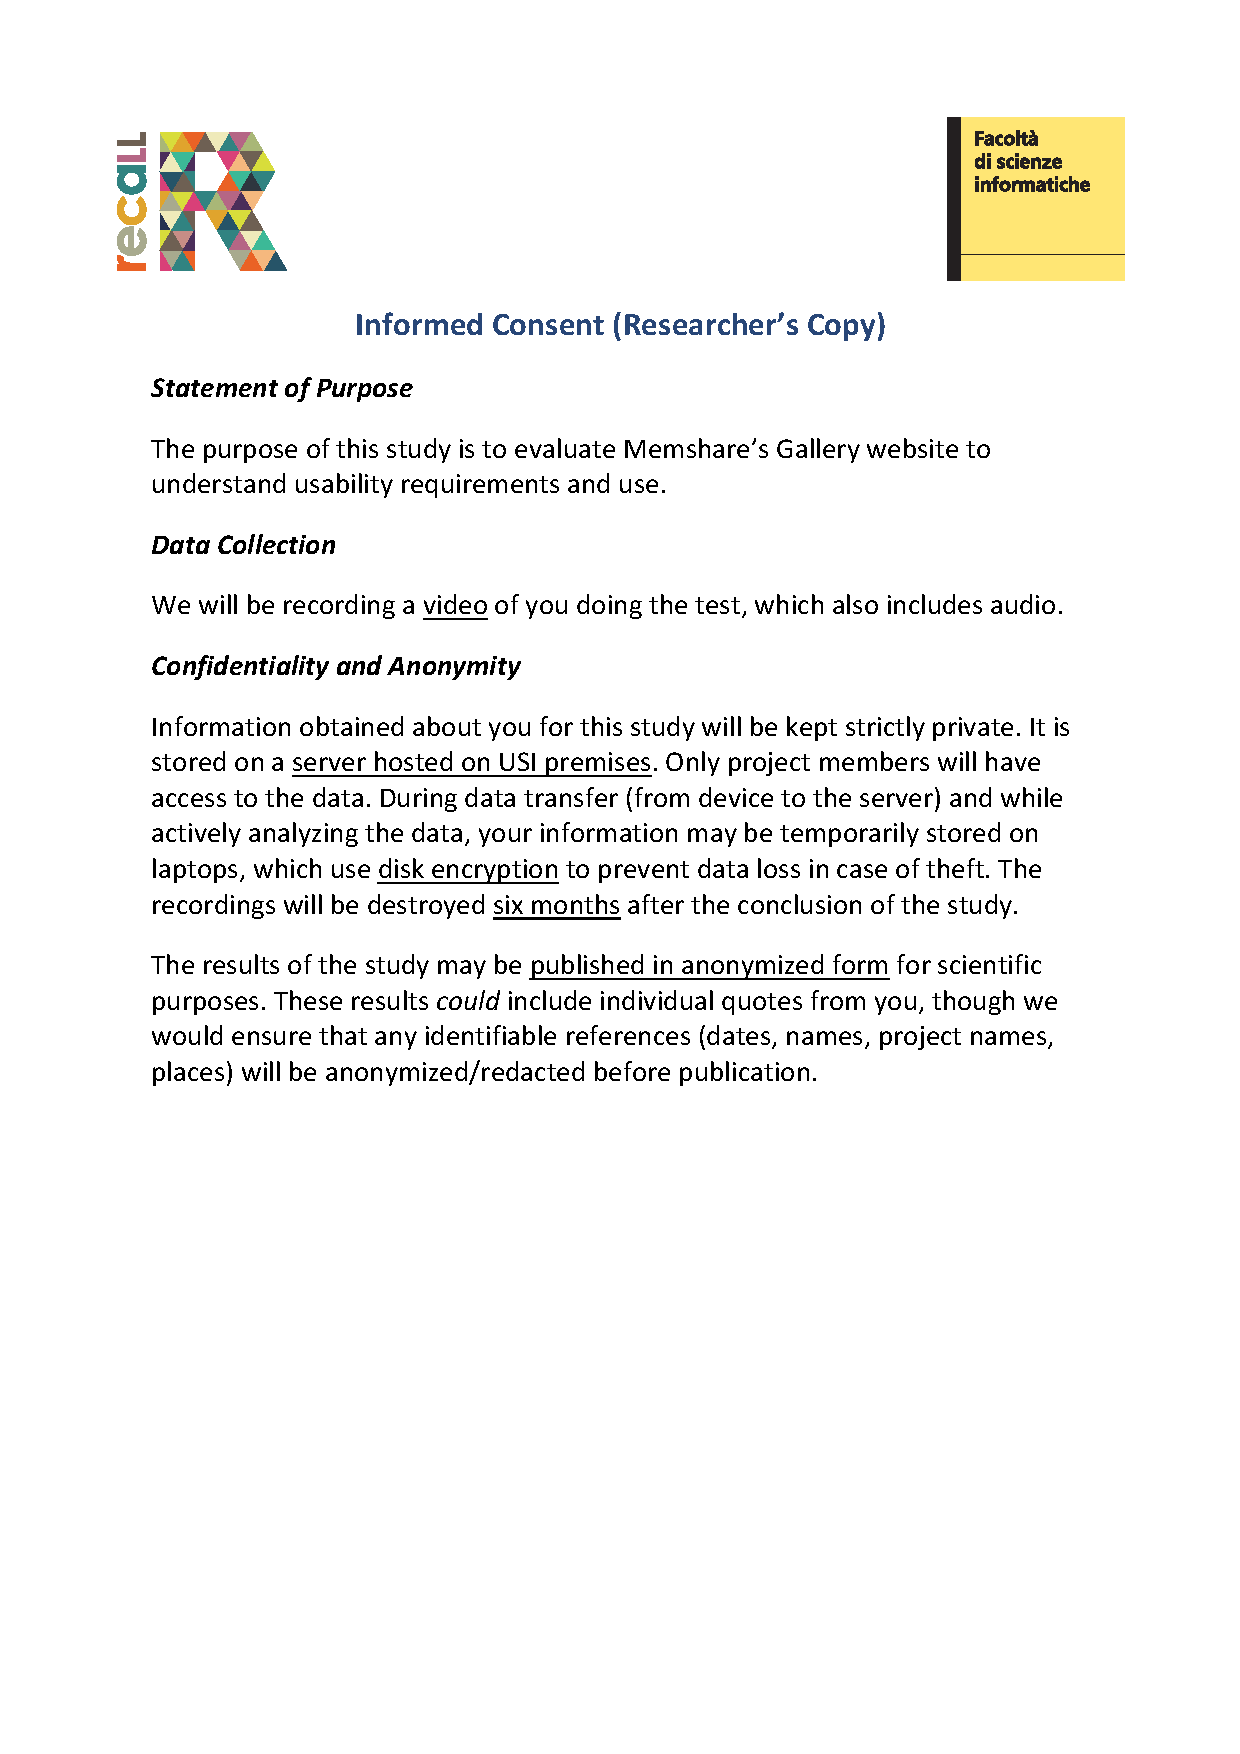
\includepdf[scale=0.8,pages=1,pagecommand=\section{Consent form}]{Consent1}
\includepdf[scale=0.8,pages=2-,pagecommand={}]{Consent1}
\label{sec:consent}

\section{Session introduction}
\label{sec:sess}
For introducing the participant to the session this script was used.
\linebreak
"Thank you for agreeing to take part in my research study. My name is Jacob, this research study is part of my master thesis for which I am working with professor Marc Langheinrich.

Today, I am asking you to serve as an evaluator for our web site that I am working on.

During the session, I will ask you to use the website to do a variety of tasks and I will ask some questions.

I will both audio and video record your reactions and comments to the Web site that you will review. 

During this session, I would like you to think aloud as you work to complete the tasks. I will not be able to offer any suggestions or hints, but from time to time, I may ask you to clarify what you have said or ask you for information on what you were looking for.
Please try to think out loud while you're working. Just tell me whatever is going through your mind. Please know that we're not testing you, and there is no such thing as a wrong answer. You're doing this helps us understand what works or doesn't work about the site.

The whole session will might take approximately 30 minutes.
Before we start this session, I would like to give a small introduction about the system I been working on. This work is part of bigger project that aims to redefine and rethink the notion of human memory augmentation. In our studies, we use images to trigger recall of past memories. For capturing these images, we use a device called narrative clip this device captures images for every 30 second and you can pin it up in your shirt. By reviewing these captured images, we believe that users will have a better memory recall. As part of this project, we have built MemShare which has two components. One is a mobile application which allows the captured images from the narrative clip to be shared among co located people vice versa (This means if you are sitting next to me your and use the same application your images will be shared with me and mine to you)  and also including any images captured from a fixed camera near the user. This will provide the user a better perspective of an event. This is because by only using the first-person perspective from the narrative clip camera you won't get a full perspective of an event, for example if you are in a meeting you might never see the person sitting next to you. The 2nd component is the MemShare's gallery website which enables you to visualize the captured images. And by reviewing these images will a help one to create more effective cues to recall their previous experience. The purpose for this session is for you to review our gallery website for our application MemShare and to get our opinions.

Do you have any questions before we begin?"

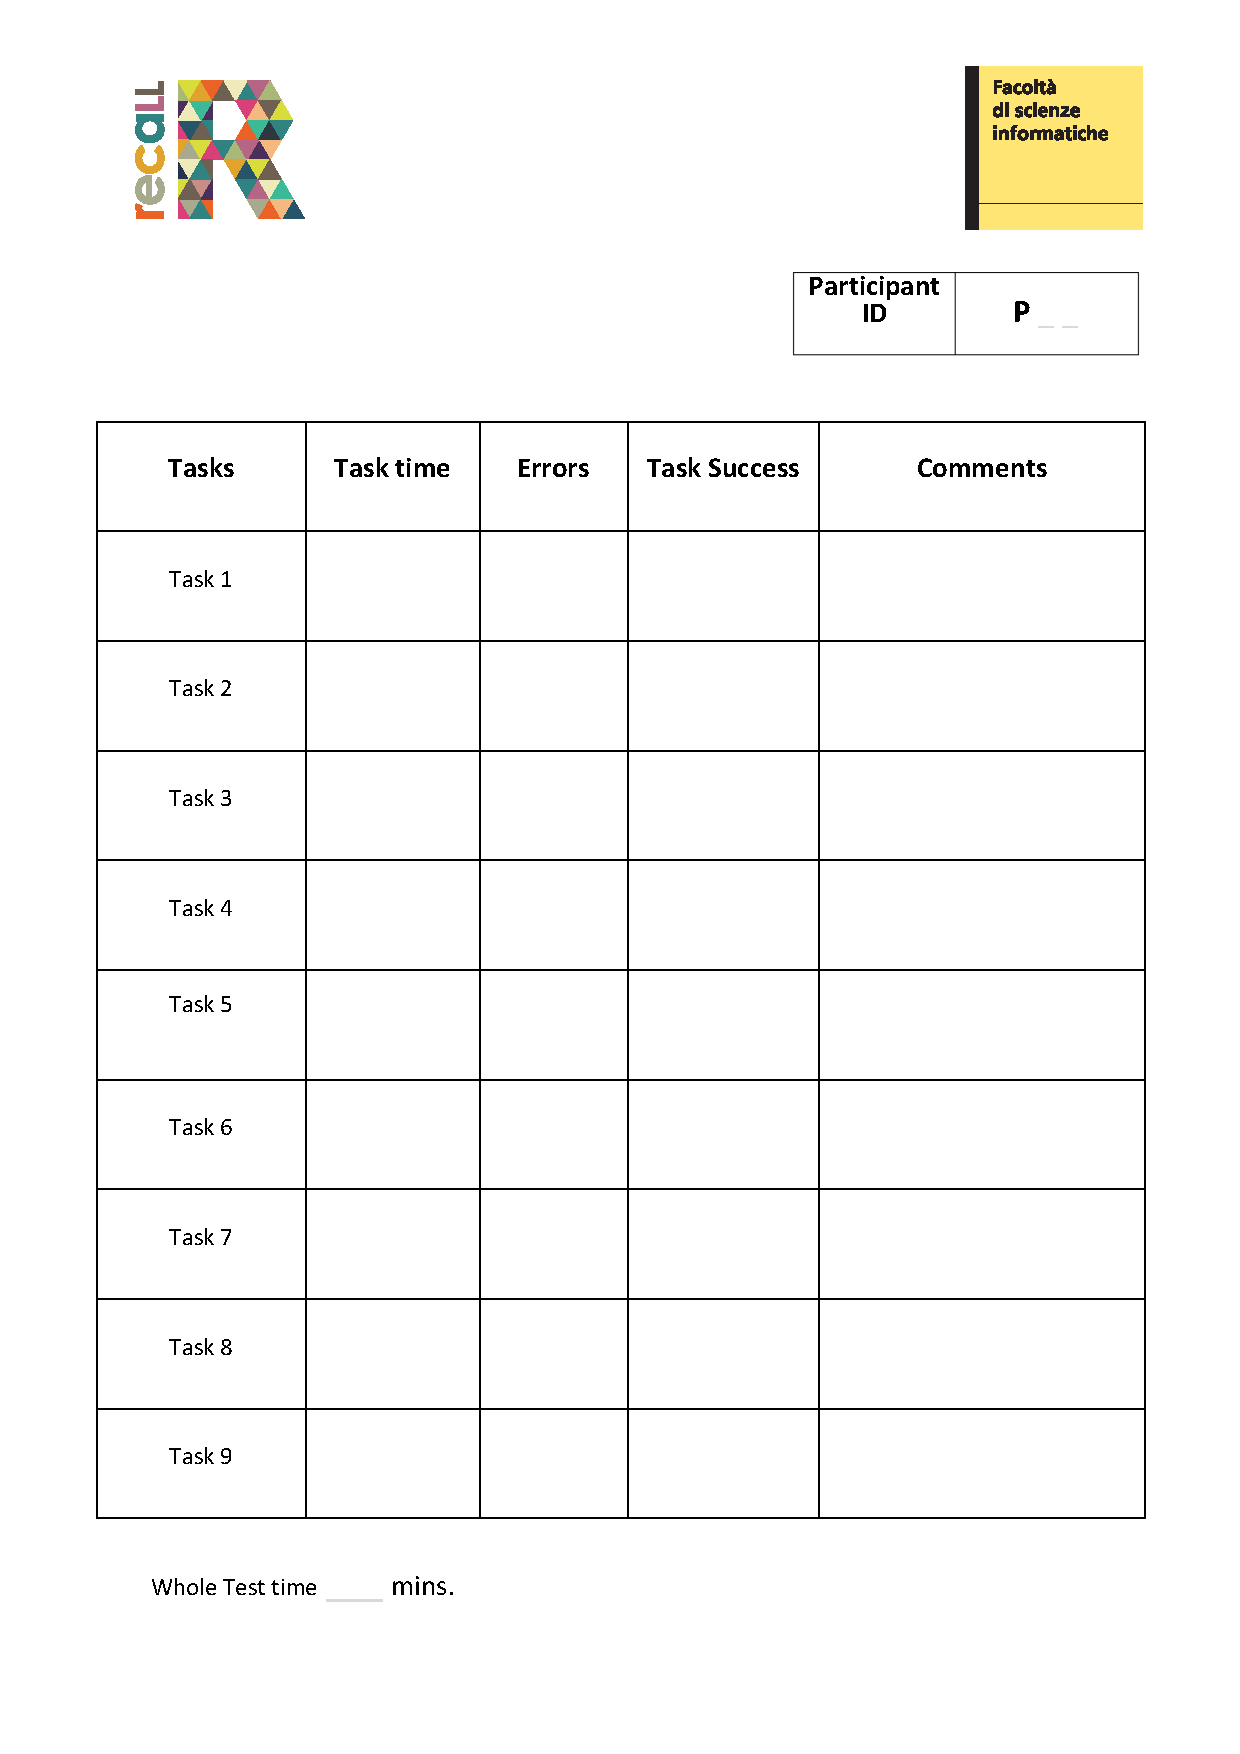
\includepdf[scale=0.75,pages=1,pagecommand=\section{Data sheet}]{Data_sheet}
\label{sec:data}

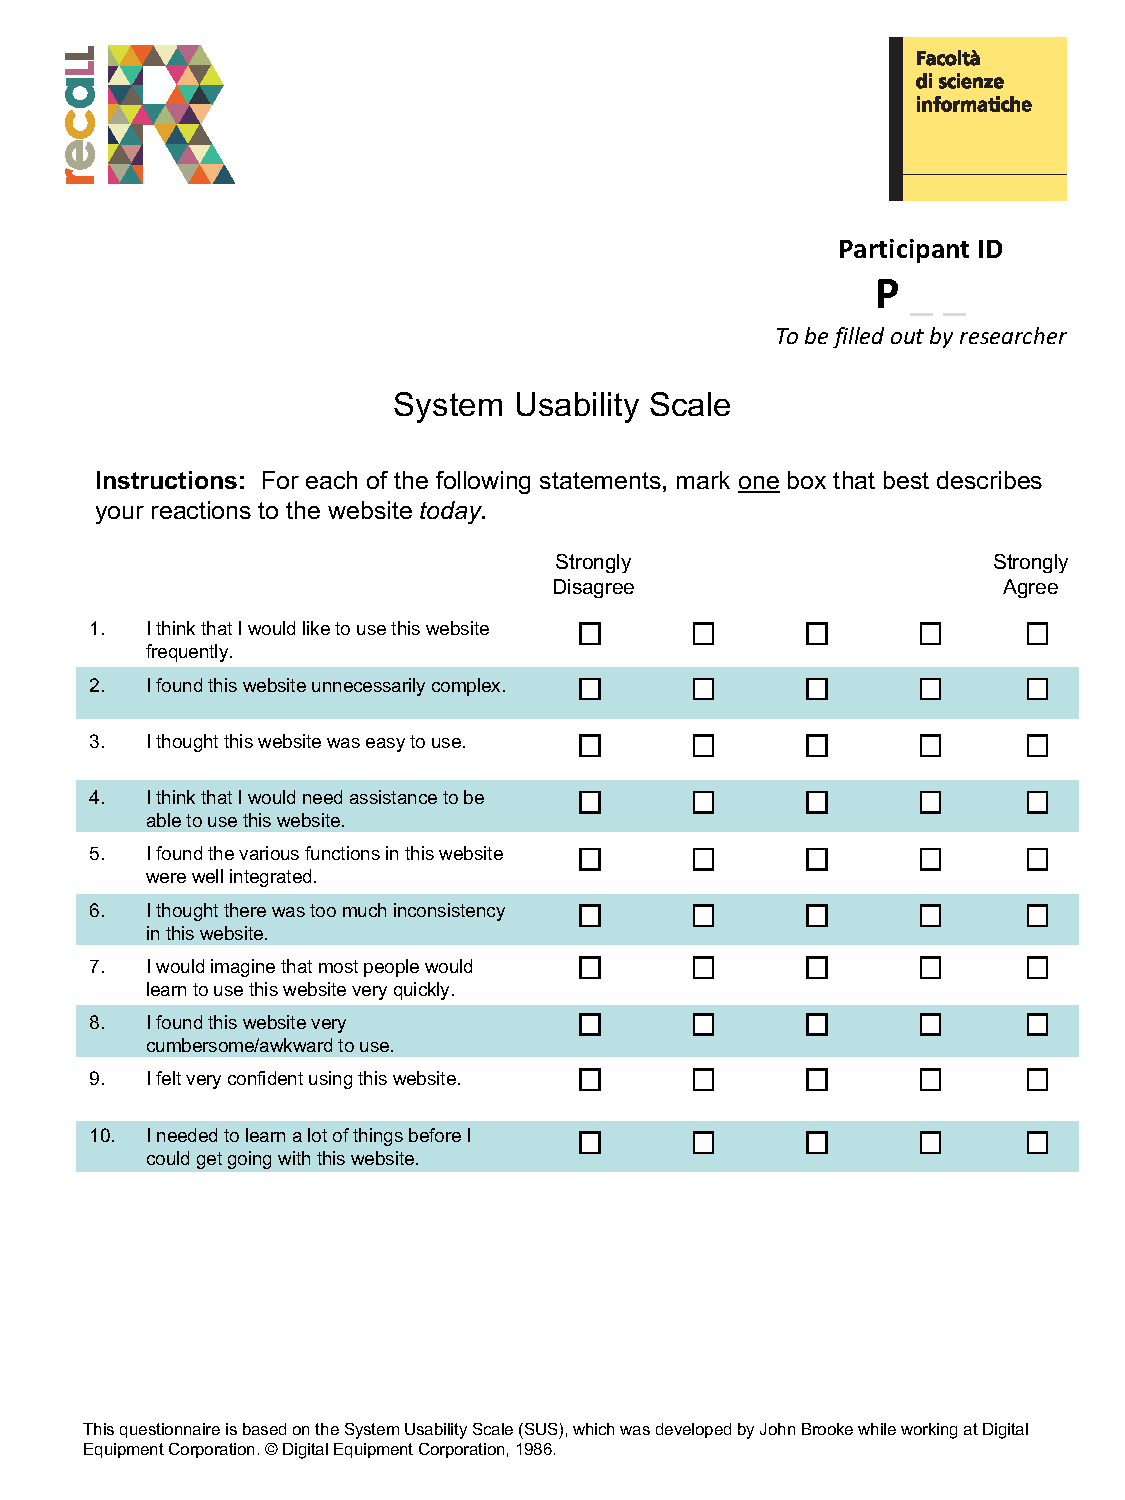
\includepdf[scale=0.75,pages=1,pagecommand=\section{SUS questionnaire}]{SUSwb}
\label{sec:sus}

\chapter{MemStone experiments contents}


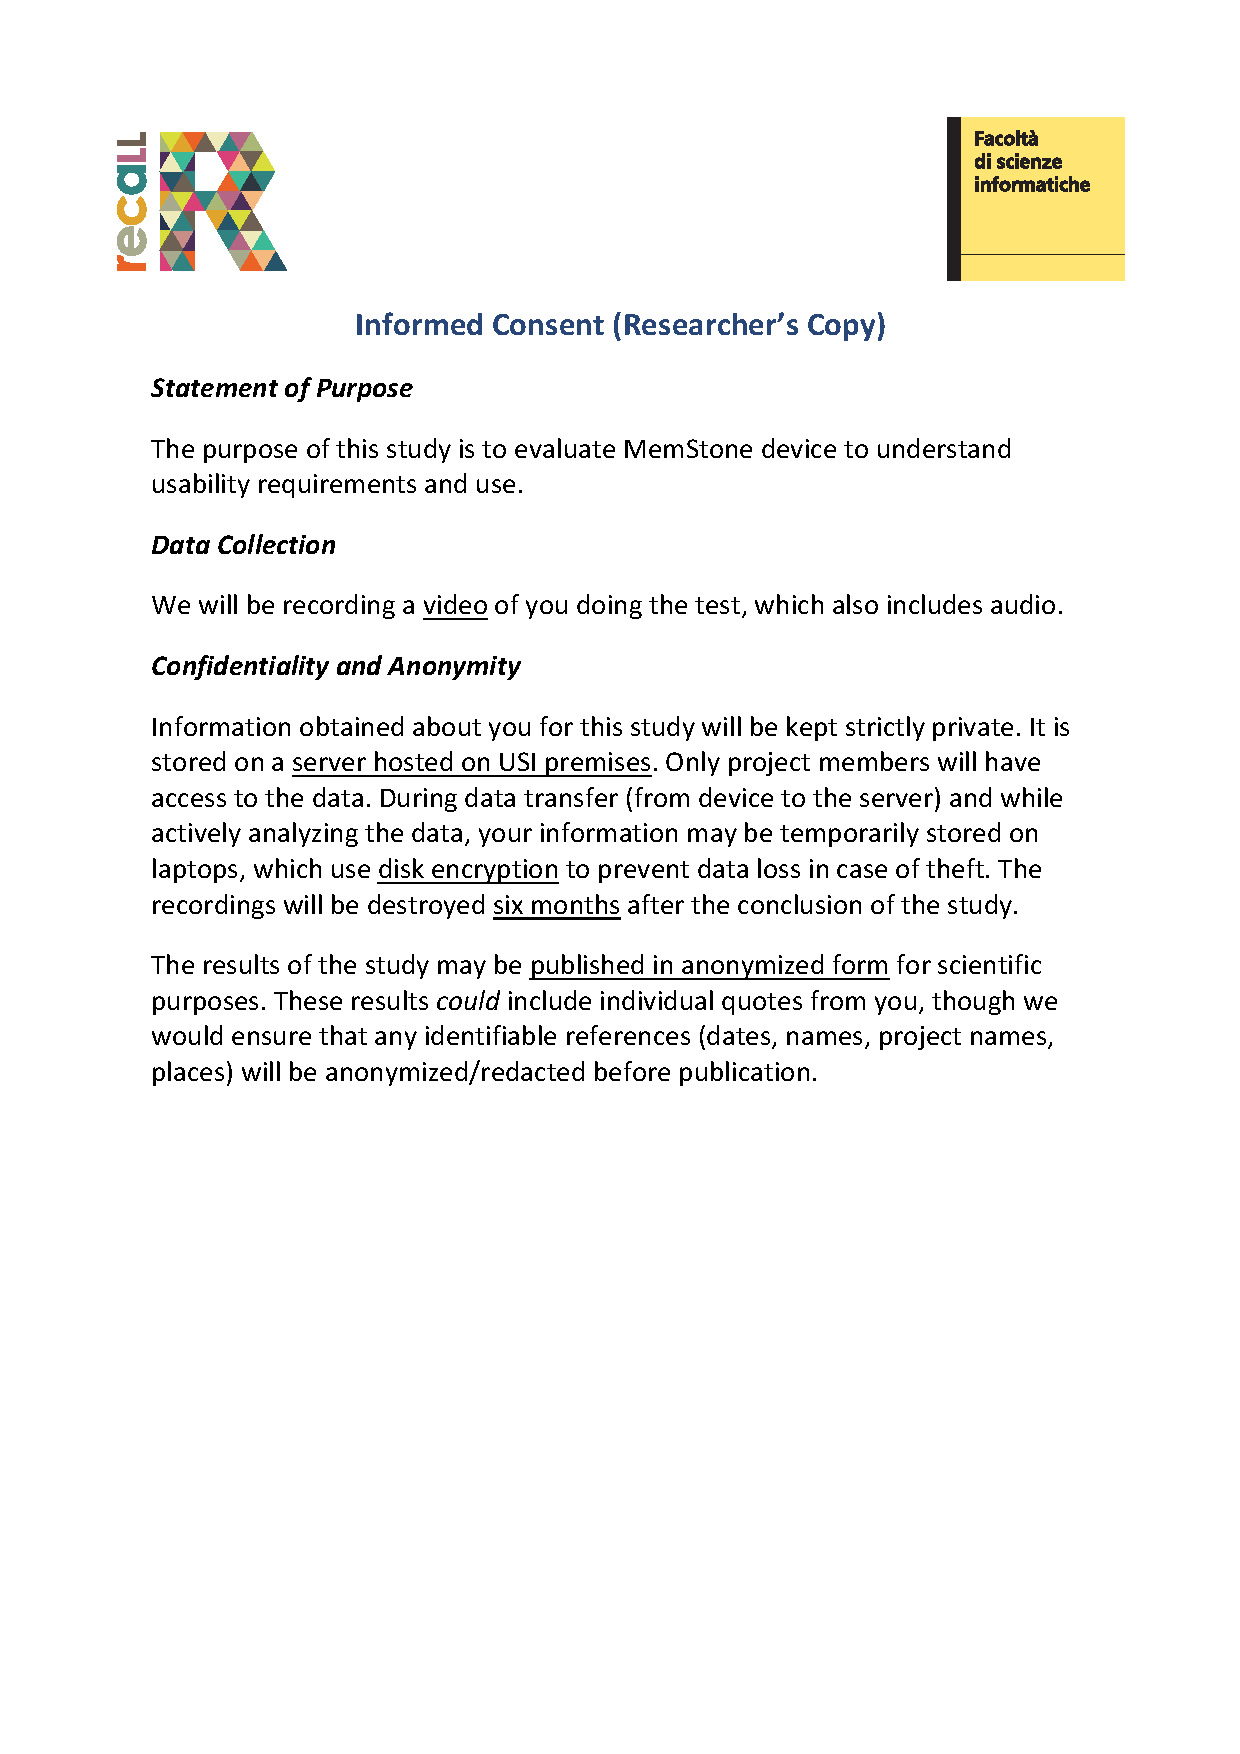
\includepdf[scale=0.8,pages=1,pagecommand=\section{Consent form}]{ConsentM}
\includepdf[scale=0.8,pages=2-,pagecommand={}]{ConsentM}
\label{ses:con}

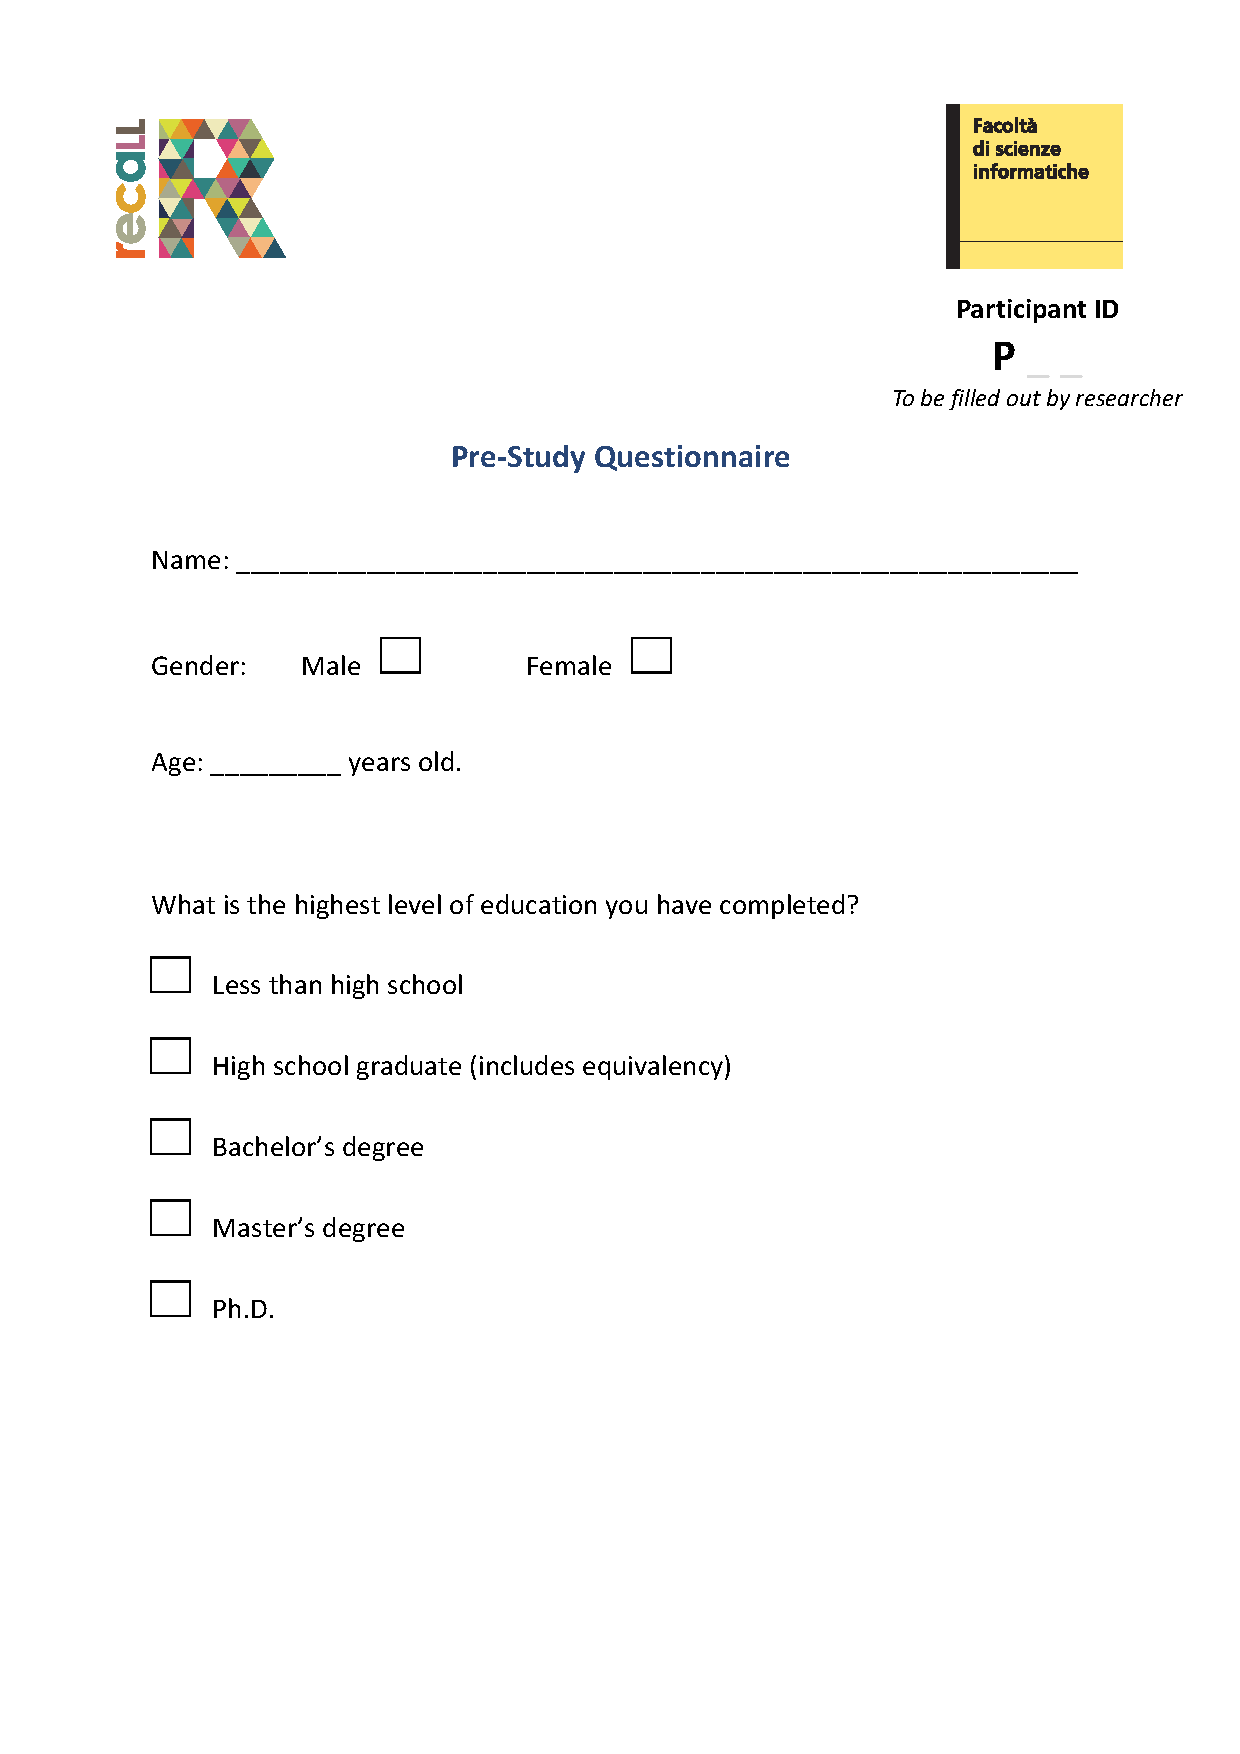
\includepdf[scale=0.8,pages=1,pagecommand=\section{Pre-questionnaire}]{Preq}
\includepdf[scale=0.8,pages=2-,pagecommand={}]{Preq}
\label{ses:pre}

\section{Session Introduction}
\label{ses:intro}
For introducing the participant to the session this script was used.
\linebreak

"Thank you for agreeing to take part in my research study. My name is Jacob, this research study is part of my master thesis for which I am working with professor Marc Langheinrich. 
Today, I am asking you to serve as an evaluator for our MemStone Interface.
Before we start this session, I would like to give a small introduction about my Project. This work is part of bigger project that aims to redefine and rethink the notion of human memory augmentation. In our studies, we use images to trigger recall of past memories. For capturing these images, we use a device called narrative clip. This device captures images for every 30 second and you can pin it up in your shirt. By reviewing these images, we believe that users will have a better memory recall. As part of this project, we have built two components. One of the component is called MemStone Interface which has 2 functions, one of the function is to allow the captured images from the narrative clip to be shared among co-located people vice versa. This will provide the user a better perspective of an event. This is because by only using the first-person perspective from the narrative clip camera you won't get a full perspective of an event, for example if you are in a meeting you might never see the person sitting next to you. The other function is to control what you share and capture, for example when you are in meeting and if you are checking phone your personal content can be shared with other co-located people to avoid this you can delete the captured picture and it won't be shared it with other co-located people or in the scenario if you are checking your laptop in middle of the meeting and you don't want to capture or share the data this device can be used. The second component is the MemShare website which enables you to visualize the captured images (which we won't be testing). We have built two versions of the MemStone Interface one is the physical device called MemStone device and another one is an smartphone application. The purpose for this session is for you to evaluate our MemStone device and smartphone application. During this study, we will have separate training session for the device and application where I will let you to use both and I will explain about different gestures and functions present in the device and application to control what you share and capture.
After the training session, I will let you to watch a video showing a meeting scripted between a professor and his TA (Teaching Assistant). I would like you to imagine yourself as the TA and use the device according to the scenario showed in the video. There will be some audio or visual clue in the video for using the right gesture or function of the MemStone Interface. After the whole session is over, I will ask some questions related to your experience of using the device and phone application. I will both audio and video record the whole session while you do the task. The whole session will might take approximately 1 hour 30 minutes. Do you have any questions before we begin?"


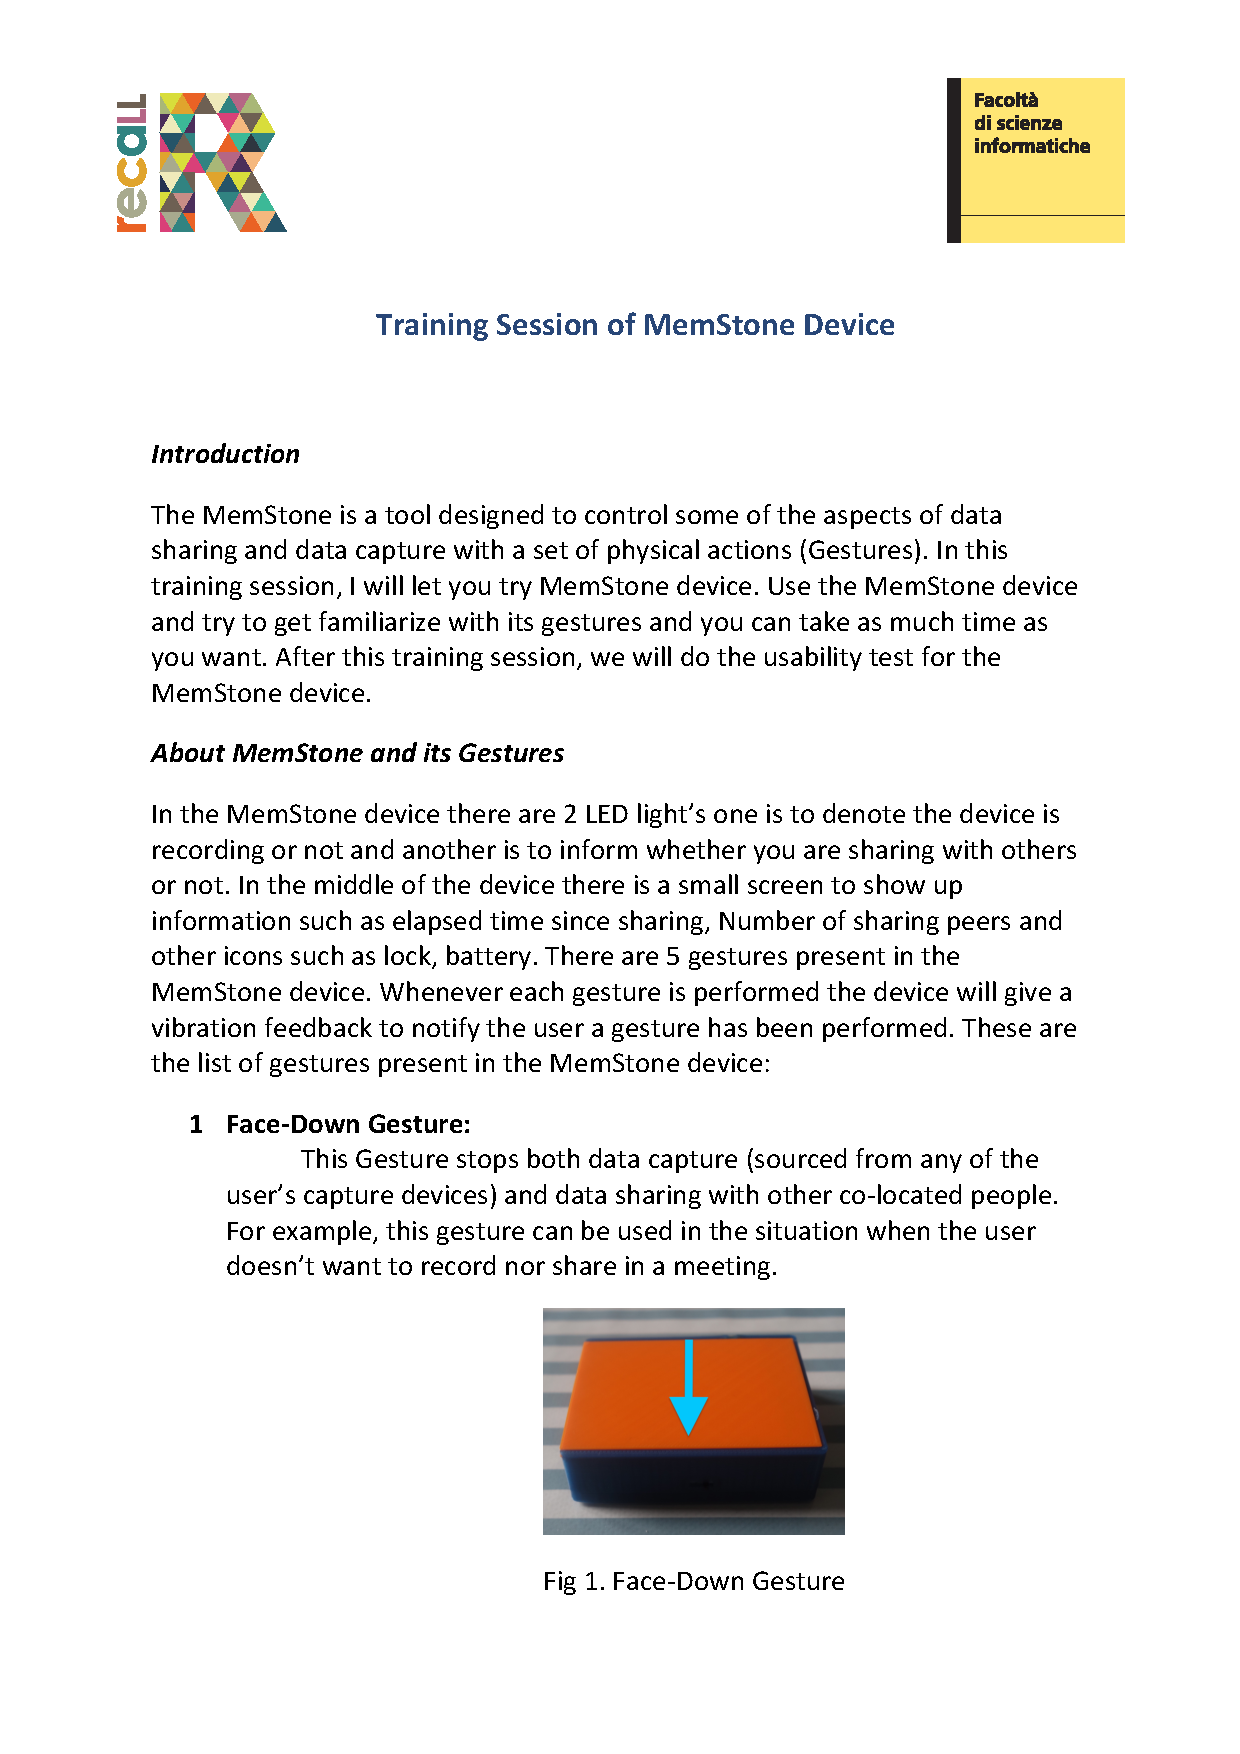
\includepdf[scale=0.70,pages=1,pagecommand=\section{Training session documents}\subsection{Training document for MemStone device}]{Memstone}
\label{ses:tra}

\includepdf[scale=0.8,pages=2-,pagecommand={}]{Memstone}

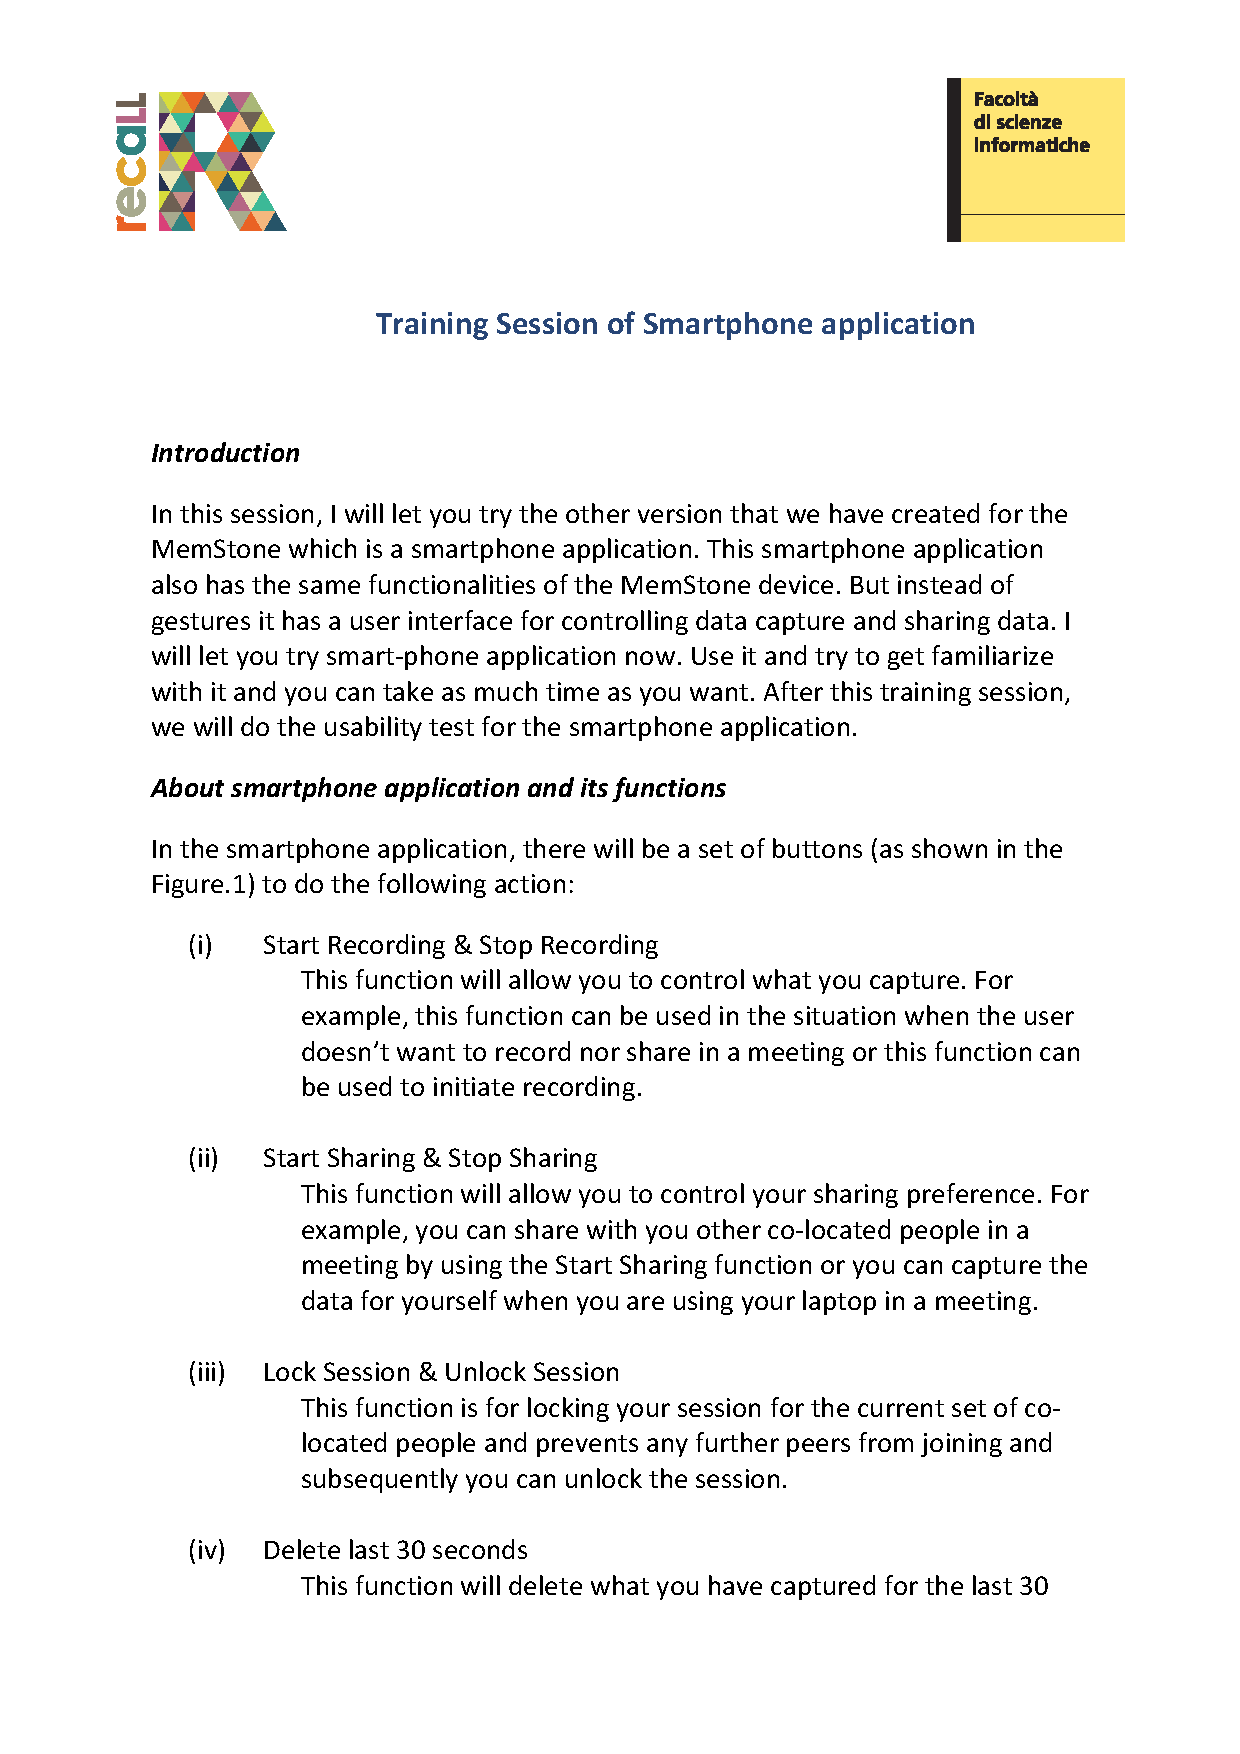
\includepdf[scale=0.8,pages=1,pagecommand=\subsection{Training document for smartphone application}]{Phone}
\includepdf[scale=0.8,pages=2-,pagecommand={}]{Phone}

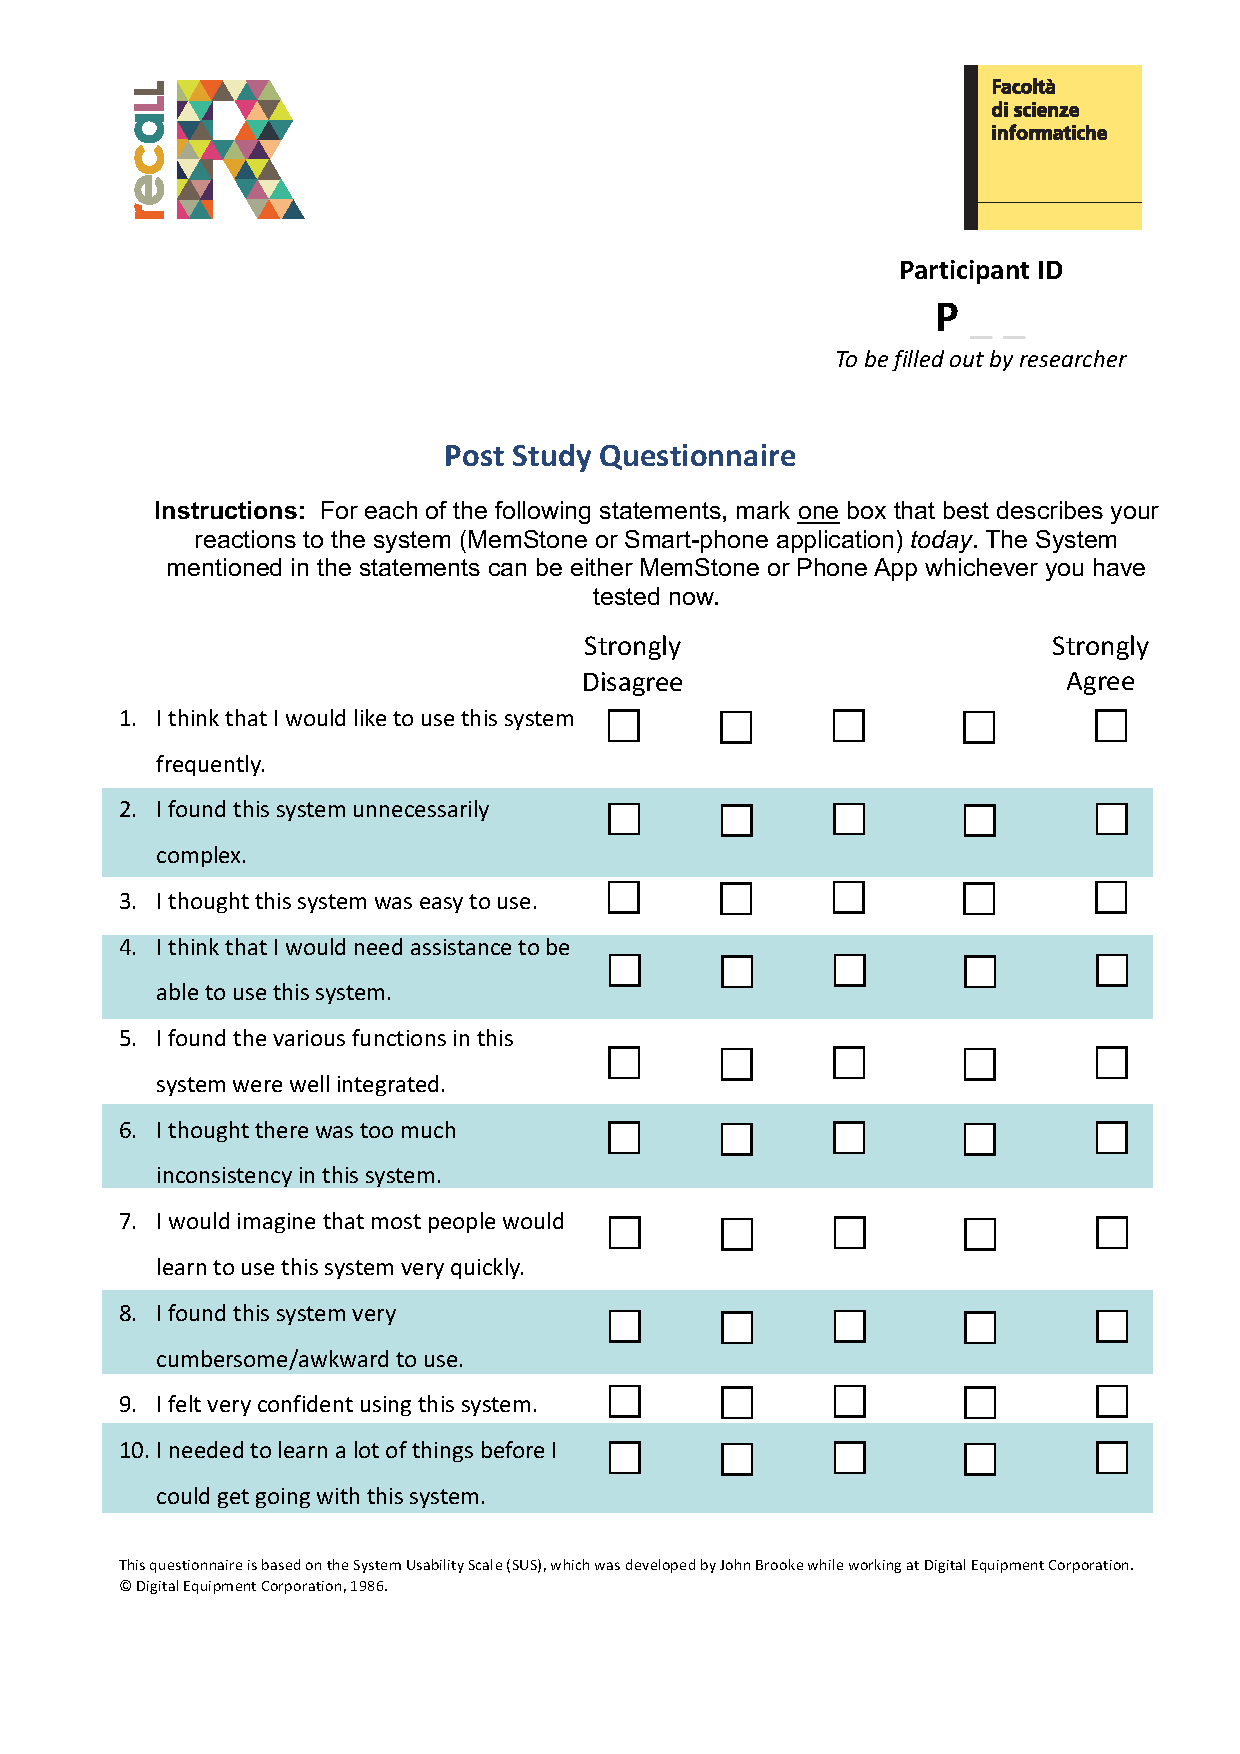
\includepdf[scale=0.75,pages=1,pagecommand=\section{Post-questionnaire}]{Postq}
\includepdf[scale=0.8,pages=2-,pagecommand={}]{Postq}
\label{ses:postq}

\section{Interview questions}
\label{ms:int}

These are the list of questions asked during the interview session : 
\begin{enumerate}
\item What is your opinion about capturing and sharing meeting information through images?
\item What is your overall impressions of the MemStone device?
\item What do you think about the Phone App? Which one would like to use in the future?Is there any gesture that you felt which was difficult to remember/to perform/or that you didn't like?
\item Did the MemStone device give appropriate feedback and displayed the needed information to you? What additional data would you like to see?
\item If you are performing the gestures in front of other participants in a meeting, do you think that you are influencing other participants in their data sharing decisions?
\item Do you think that MemStone allows you to securely share your captured data with others (e.g. you only share with meeting attendants and with no other people)?
\item What about your privacy? By using the MemStone device, do you think that you are able to control what data you share with others, and prevent sharing of sensitive data?
\item Does the Phone Application provide you with the same level of security and privacy control?
\item Do you have any other questions or comments about the MemStone device?
\item Do you have any suggestions or changes that you want to make in the MemStone device?
\end{enumerate}

\chapter{Transcripts}
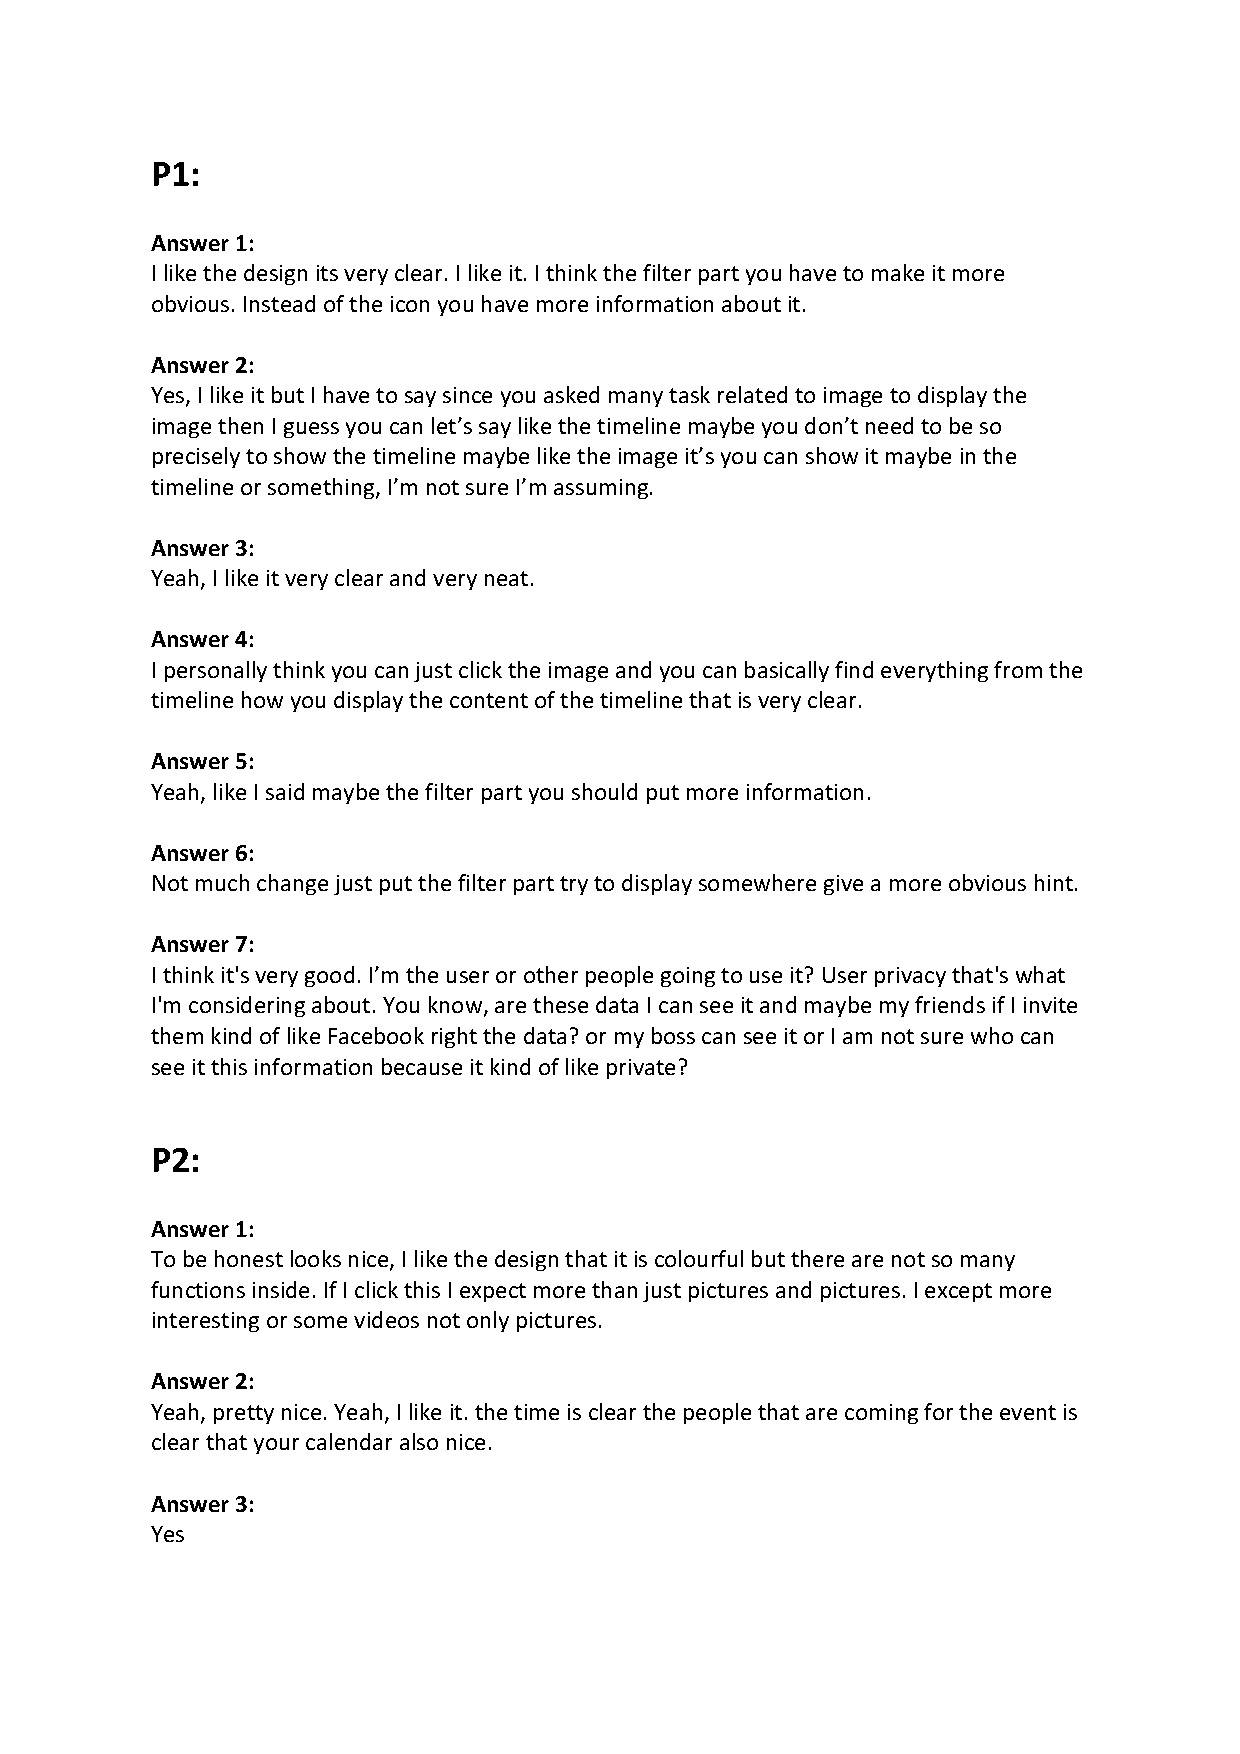
\includepdf[scale=0.85,pages=1,pagecommand=\section{MemShare evaluation interview transcripts}]{transwb}
\includepdf[scale=0.85,pages=2-,pagecommand={}]{transwb}
\label{mem:trans}

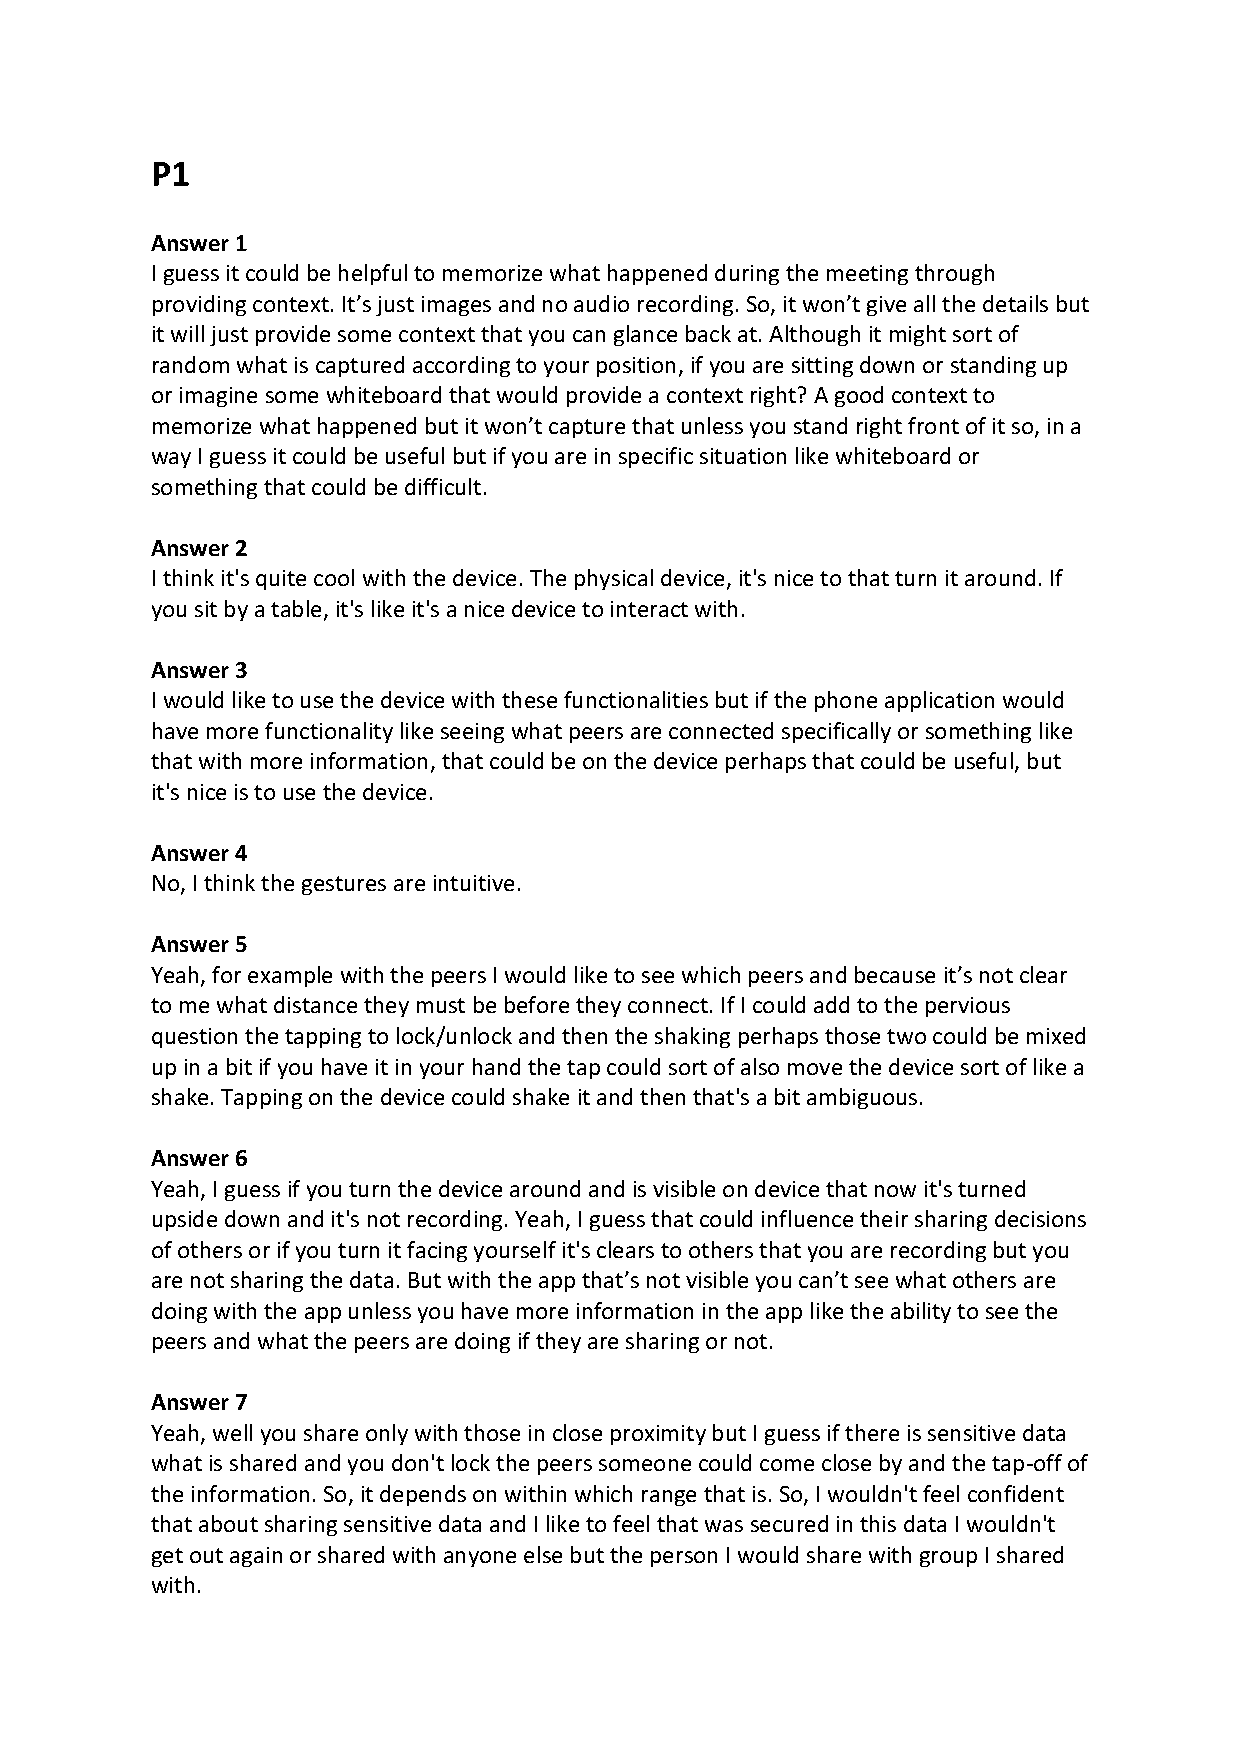
\includepdf[scale=0.85,pages=1,pagecommand=\section{MemStone evaluation interview transcripts}]{memt}
\includepdf[scale=0.85,pages=2-,pagecommand={}]{memt}
\label{mem:mt}


\backmatter

%\bibliographystyle{alpha}
%\bibliographystyle{dcu}
\bibliographystyle{plainnat}
\bibliography{Biblo1}

%\cleardoublepage
%\theindex %optional, use only if you have an index, must use
	  %\makeindex in the preamble


\end{document}
